\documentclass[12pt]{article}
\usepackage[utf8]{inputenc}
\usepackage{amsmath}
\usepackage{amsfonts}
\usepackage{amssymb}

\usepackage[margin=1in]{geometry} %1inch margins
\usepackage{graphicx} %for picture inclusion
\graphicspath{ {Figures/} }
\usepackage[backend=bibtex]{biblatex} %for references
\addbibresource{ref.bib} % bibliography info file
\usepackage{authblk} %for titles
\usepackage{verbatim}

\begin{document}

\author{Daniel Gawerc\\Mentor: Maria Spiropulu\\Co-Mentor: Cristian Peña}
\affil{California Institute of Technology}
\title{Progress Report \#2}
\date{29 July 2016}
\maketitle

\section{Background}
At the Large Hadron Collider (LHC), the High Luminosity upgrades plan to achieve luminosities of greater than $10^{34}$ cm$^{-2}$s$^{-1}$, with 140 – 200 pileup events per bunch crossing every 25 ns \cite{P1}. 
Because of the physical spread of each bunch, the collisions occur over a large region rather than at an isolated point, which leads to a spread in time ($\sim$ 200 ps) \cite{P1}. 
Thus, detectors in the calorimeter must have a good (low) time resolution in order to resolve individual collisions. 
In order to reconstruct the vertex of a collision with an increased pileup, the electromagnetic calorimeter (ECAL) detectors should have a time resolution of about 10 ps \cite{P1}.


\section{Experimental Setup}
This summer, the Caltech Precision Timing group took data at the Fermilab Test Beam Facility (FBTF). 
The experiment involves placing different calorimeter detectors in the beam line, in order to observe how the addition of detectors in the perpendicular transverse plane and/or parallel longitudinal direction along the beam line will improve the overall detector time resolution. 
The layers of detectors are meant to mimic the proposed High Granularity Calorimeter (HGC) detector, which shall replace the CMS ECAL endcap, and is described in detail below \cite{P2}. 
The results of this research may be useful in preparing the LHC High Luminosity upgrades.

In the FTBF experiment, different types of detectors were utilized. 
In the front of the setup, a scintillator crystal and PMT are used as a trigger. 
Depending on the configuration, there are a few radiation lengths ($X_0$) of either lead or tungsten absorbers behind the PMT in order to spread out and propagate the particle shower and produce more secondary electrons and photons. 
A depiction of the setup is given in Figure \ref{fig:setup}.

\begin{figure}[h]
	\centering
	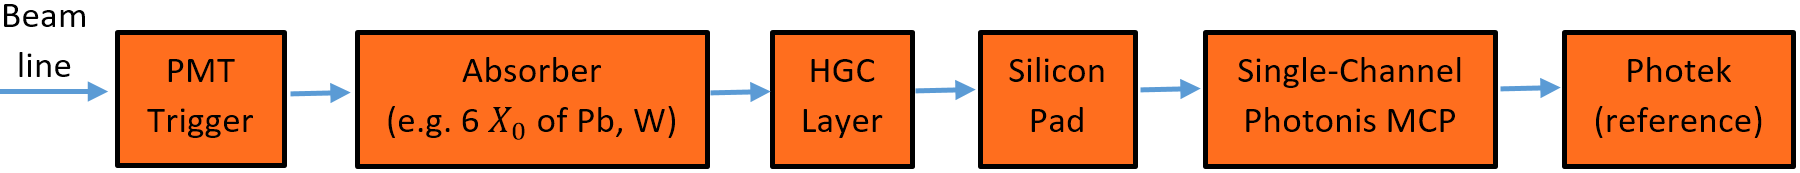
\includegraphics[width=\linewidth]{setup.png}
	\caption{A typical experiment configuration.}
	\label{fig:setup}
\end{figure}

\begin{figure}[h]
\centering
\begin{minipage}[t]{.5\textwidth}
	\centering
	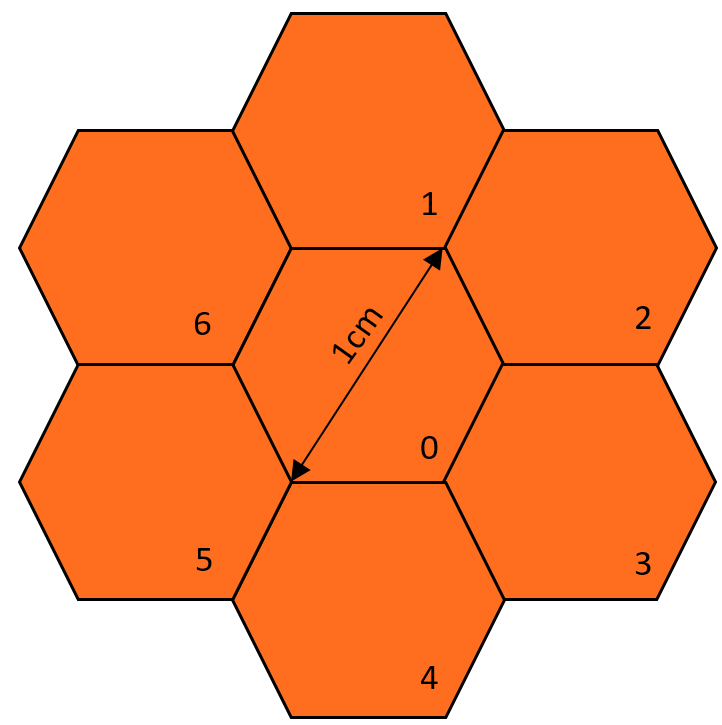
\includegraphics[scale=0.5]{HGC.png}
	\caption{A depiction of the innermost 7 pixels of the HGC layer. 
	The actual board has more than 7 pixels in a single layer.}
	\label{fig:HGC}
\end{minipage}
\end{figure}

The High Granularity Calorimeter (or PicoSil when referring to a single pixel’s readout that has been optimized for timing) layer has an array of separated silicon pixels, in a hexagonal honeycomb geometry \cite{P2}. 
A depiction of the HGC layer is given in Figure \ref{fig:HGC}. 
Because the beam is focused at the HGC center pixel (0 in Figure \ref{fig:HGC}), its signal is reduced using a 6 dB attenuator due to the high charge detected relative to other pixels. 

The Photek 240 MCP is used as a reference detector because its time resolution is good ($\sim$ 10 ps). 
Because the readout board for all the detectors is divided into 4 groups, which have some time delay between them, the Photek signal is split into 4 cables and plugged into each group as the reference signal from which the TOFs (time of flight, or $\Delta t$) are calculated. 
Specifically, the time taken for the particle to travel from a device to the reference Photek - the time of flight – is represented by $\Delta t$. 
In the data analysis, the $\Delta t$ values over all events in the run (with certain \textit{bad} events excluded) are combined in a histogram, forming a Gaussian peak. 
The peak $\sigma$ parameter is denoted the time resolution.

There is a 64-channel and a single-channel Photonis MCP. 
The 64-channel Photonis was not present for most runs, and the single-channel Photonis was instead used. 
Lastly, a silicon pad (SiPad) detector was present for most runs, however it only detected pulses well in the very early runs, and does not seem to be useful in most of the analysis.

\section{Data Analysis}
This section aims to explain the general data analysis methods discussed later in this report.

\subsection{Data Analysis: Overview}
The Caltech Precision Timing group already had developed some analysis code for previous test beam experiments. 
The program \textit{dat2rootCP} analyzes the .dat files (with low-level information) from the runs and turn them into .root files containing a tree with plots and fit results (higher-level information). 
Since some of the data contained ringing noise, which often resulted in the wrong peak being identified as the pulse, \textit{dat2rootCP} was updated to correct for these events. 
Additionally, new macros were written in order to automate batch file analyses and merging the results into a single .root file (for when the setup configuration and beam type were the same over many runs). 
These programs utilize the ROOT programming language, which is based largely on C++. 
It is the main programming language used by scientists at CERN and in the field of HEP (see: root.cern.ch).  
The .root file extensions are associated with the ROOT language.

Because the HGC layer has multiple pixels, each pixel detects different signals and has a different time resolution. 
The \textit{MultiChannelStudy} code was created (here channel and pixel are used interchangeably), which calculates and combines the TOF ($\Delta t$) histograms for different pixels in order to return a better overall time resolution. 
The $\Delta t$ values are calculated for every event in a run by subtracting the pulse time in one device from the pulse time in the Photek (making sure that it is from the same cabling group 1-4 as the device). 
A 1-D histogram is then filled event-by-event with the $\Delta t$ values. 
In an ideal world with perfect detectors and no variation in each event, the histogram would be a Dirac delta function with a time resolution of zero. 
However, due to detector jitter, the signal-to-noise ratio and the particle shower development in the material will vary event-by-event, resulting in Gaussian TOF histograms \cite{P2}. 
After fitting the histogram to a Gaussian, the $\sigma$ parameter gives the time resolution of the detector/pixel. 
If weighted correctly, combining the HGC pixels’ $\Delta t$ histograms will result in a combined histogram with better time resolution (smaller $\sigma$). 
This improvement is due to the combination of non-overlapping information about the shower size and development in each of the detectors.

Because there are also multiple devices along the beam line as well as multiple HGC pixels, the analysis of the coplanar HGC pixels has been called \textit{transverse analysis}, and the analysis of multiple devices \textit{longitudinal analysis}. 
This report shall deal mainly with the longitudinal analysis: analyzing the improvement in the time resolution when taking the HGC layer, single-channel Photonis MCP, and SiPad into account. 
However since it is best to use the time resolution from the entire HGC layer, much of the transverse analysis will be included as well. 
Due to re-cabling the wires of the detectors into different groups between runs 52 and 53, multiple longitudinal analysis codes were written for each setup. 
Additionally, the silicon pad has noise dominating for most of the runs, and substantially deteriorates the combined detector time resolution. 
For example, Figures \ref{fig:Center} and \ref{fig:MCP} give the time of flight ($\Delta t$) histograms for runs 65-83 (same configuration) for the HGC center pixel and the Photonis MCP, along with their Gaussian fit $\sigma$ parameter. 
The Gaussian fit used the log-likelihood maximization method, as the $\chi^2$ minimization method is incorrectly biased by histogram bins with few/empty events.
Figure \ref{fig:SiPad} gives the TOF histogram for the silicon pad. 
Figure \ref{fig:wctc} is one possible combination histogram (more details below on how the individual device $\Delta t$'s can be combined). 
Clearly the combined histogram improves the silicon pad resolution by about 4 times, but it is 4-5 times \textit{worse} than the individual resolutions of the HGC and MCP. 
Additionally, the silicon pad histogram is peaked, but certainly not Gaussian. 
Thus, because it is usually more favorable (in most - but not all - runs) to simply exclude the silicon pad, code that does not account for the silicon pad was also created.

Therefore, because of the change in cabling and the noise in the silicon pad, the following longitudinal analysis codes were used: \textit{MultiDeviceStudy}, \textit{MultiDeviceStudy\_InitialWiring}, \textit{MultiDeviceStudy\_PicosilMCP}, and \textit{MultiDeviceStudy\_InitialWiring\_PicosilMCP}. 
Because the most applicable file is \textit{MultiDeviceStudy\_PicosilMCP}, it is more extensive than the others, incorporating all of the ring 1 pixels (the 6 pixels surrounding the center pixel; refer to Figure \ref{fig:HGC}) in the analysis. 
Thus, the code implements transverse analysis of the HGC as well as longitudinal analysis by adding the Photonis MCP.

\begin{figure}[h]
\centering
\begin{minipage}[t]{.49\textwidth}
	\centering
	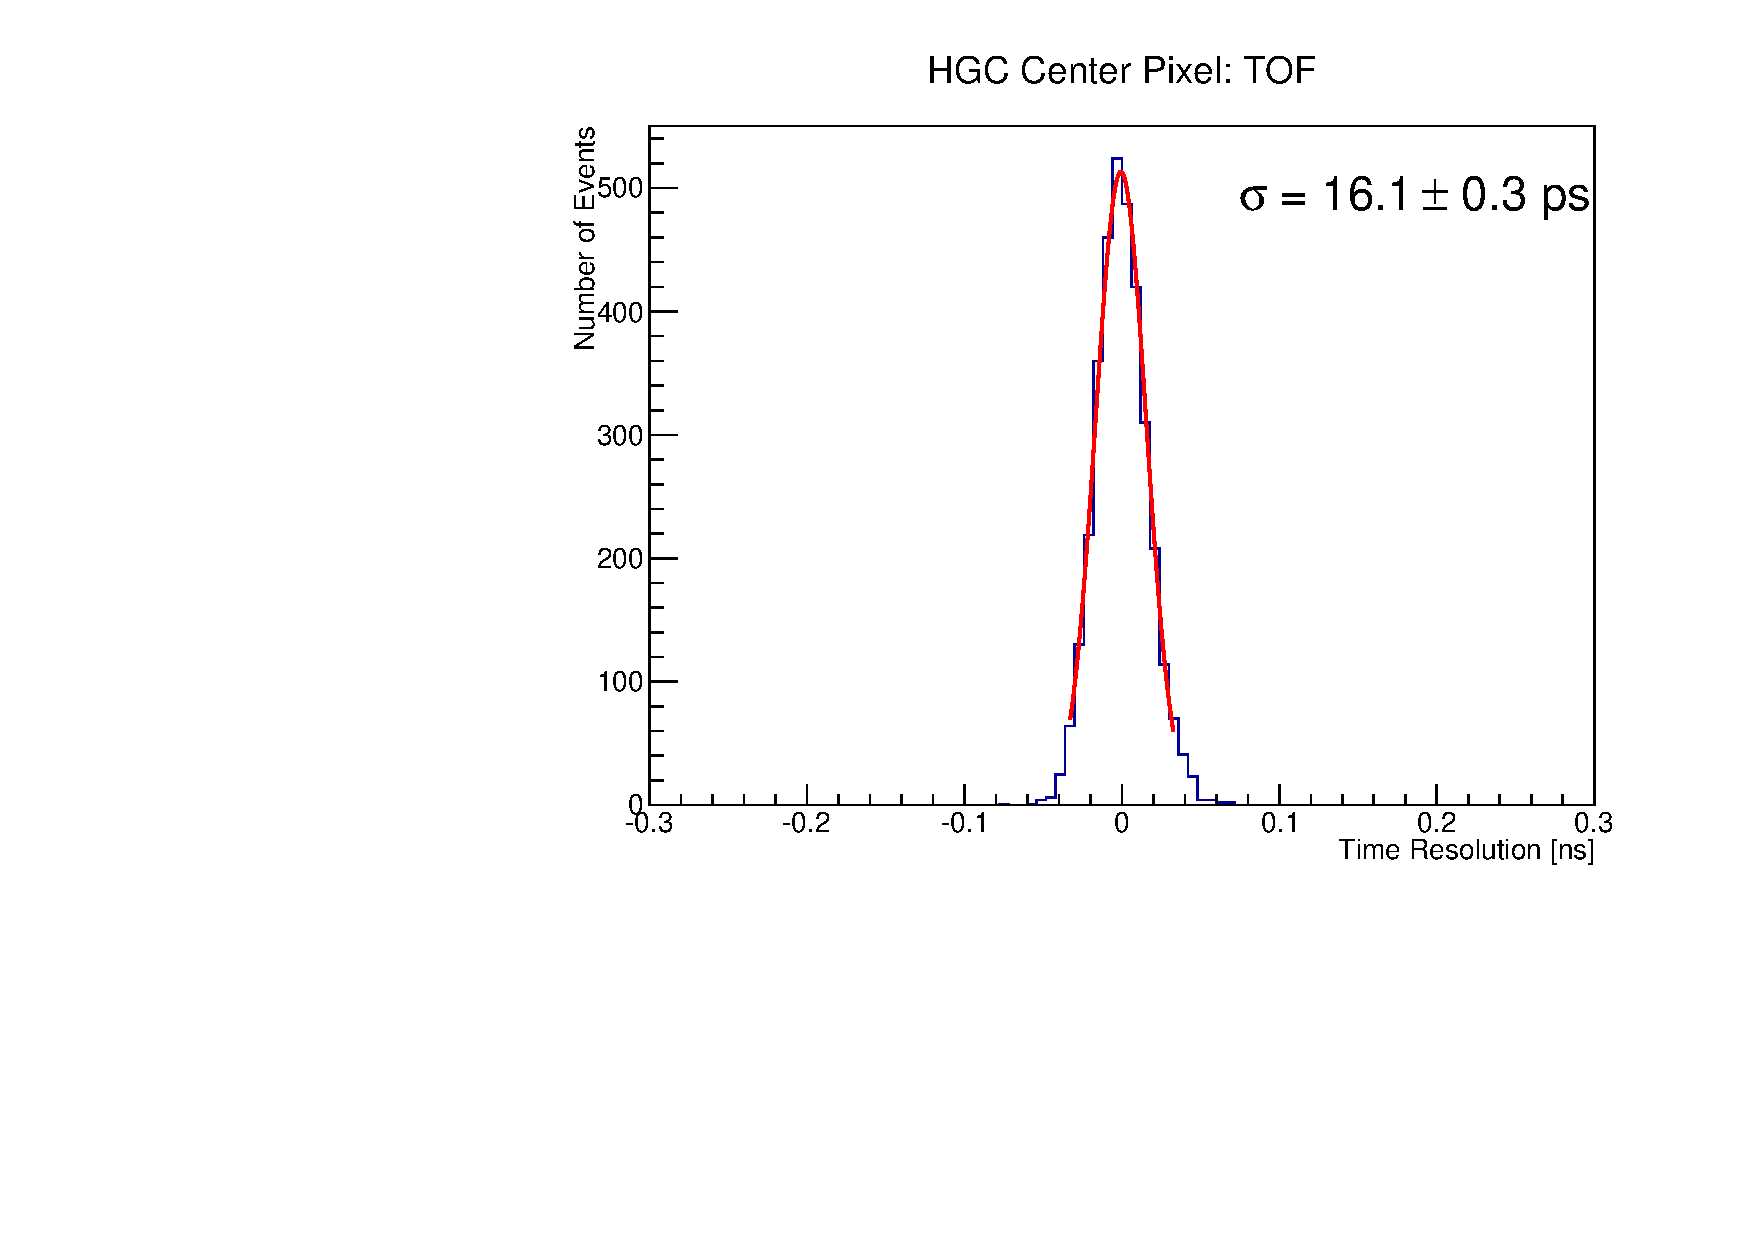
\includegraphics[width=\textwidth]{deltaTCenter.pdf}
	\caption{TOF of the HGC Center Pixel}
	\label{fig:Center}
\end{minipage} \hfill
\begin{minipage}[t]{.49\textwidth}
	\centering
	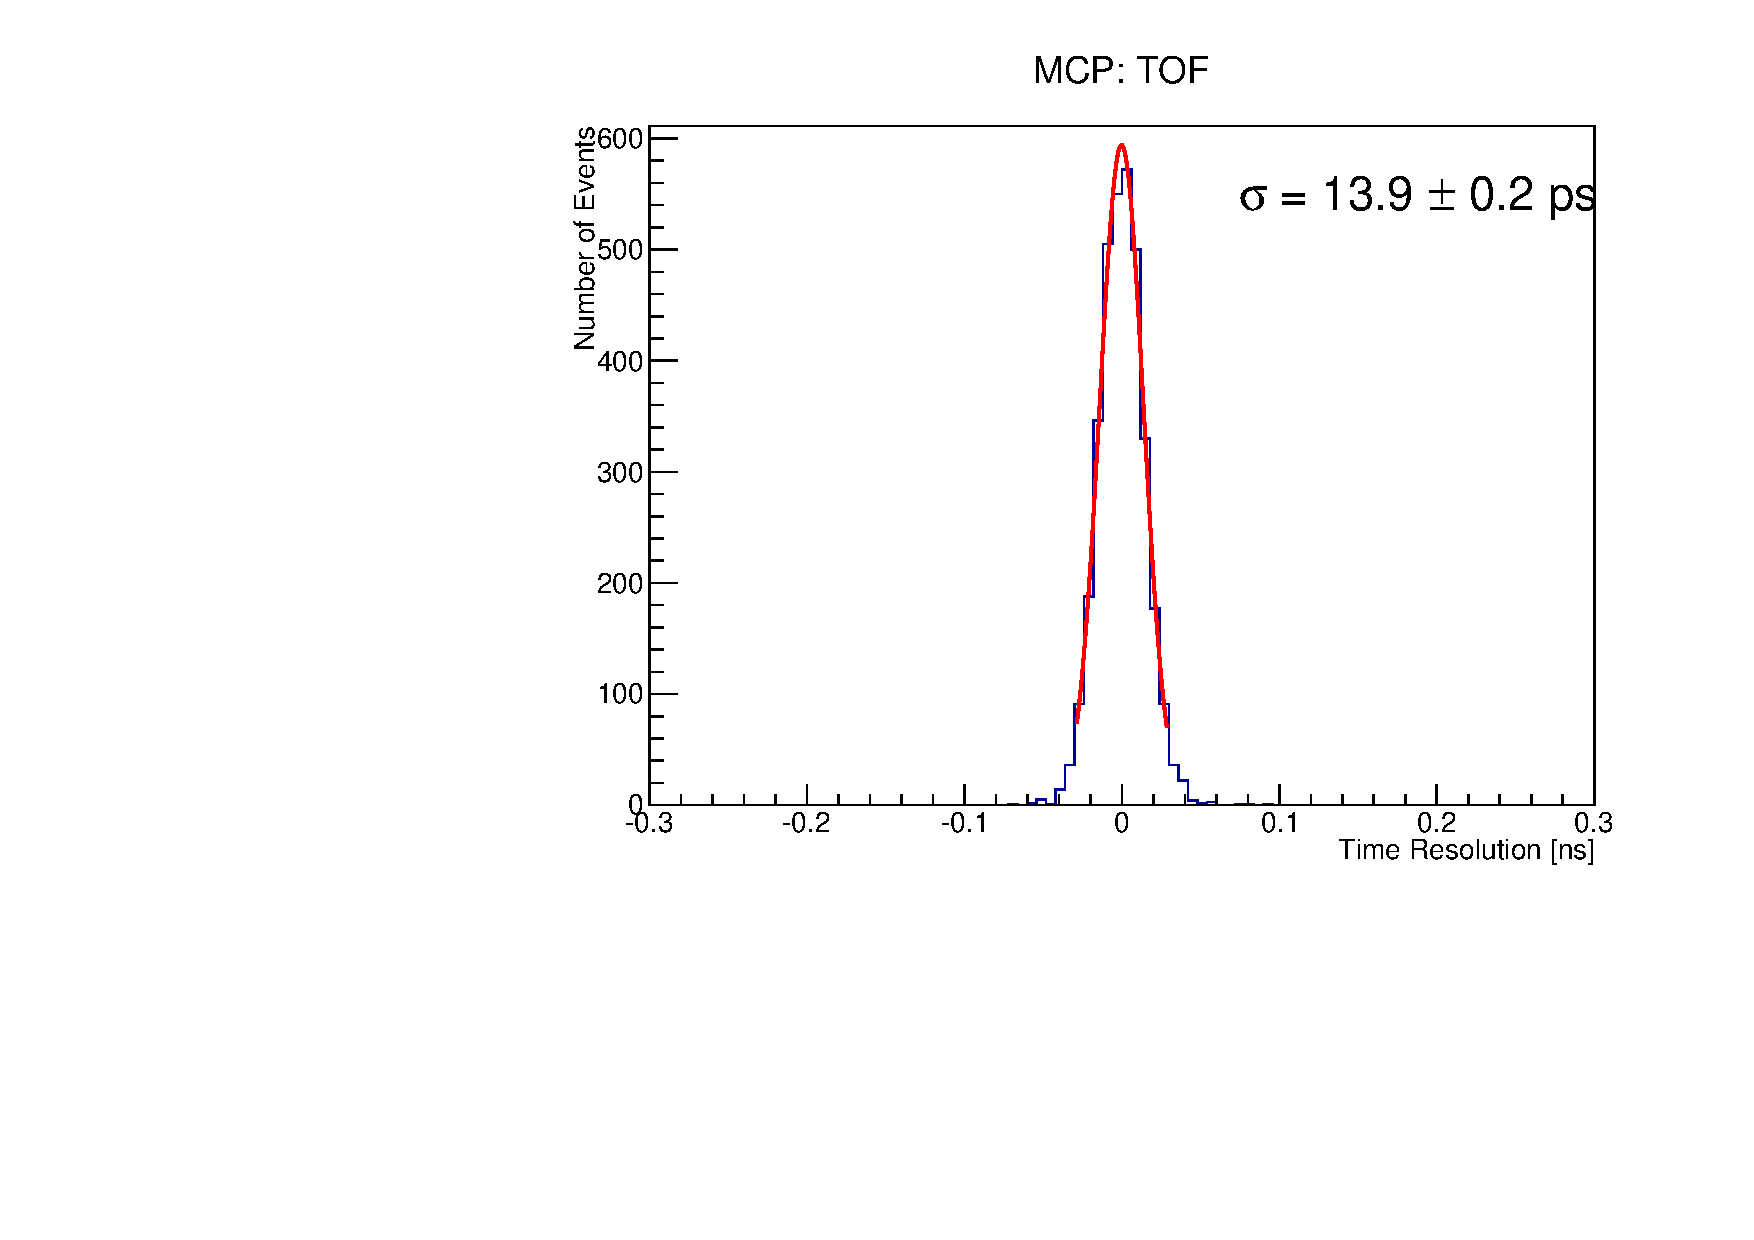
\includegraphics[width=\textwidth]{deltaTMCP.pdf}
	\caption{TOF of the Single-Channel Photonis MCP}
	\label{fig:MCP}
\end{minipage}
\end{figure}

% The following 2 plots are actually a bit out of date, and were combined with slightly
% different versions of the two above plots. Main point is still correct. Would need to
% update the below plots for any final paper.
\begin{figure}[h]
\centering
\begin{minipage}[t]{.49\textwidth}
	\centering
	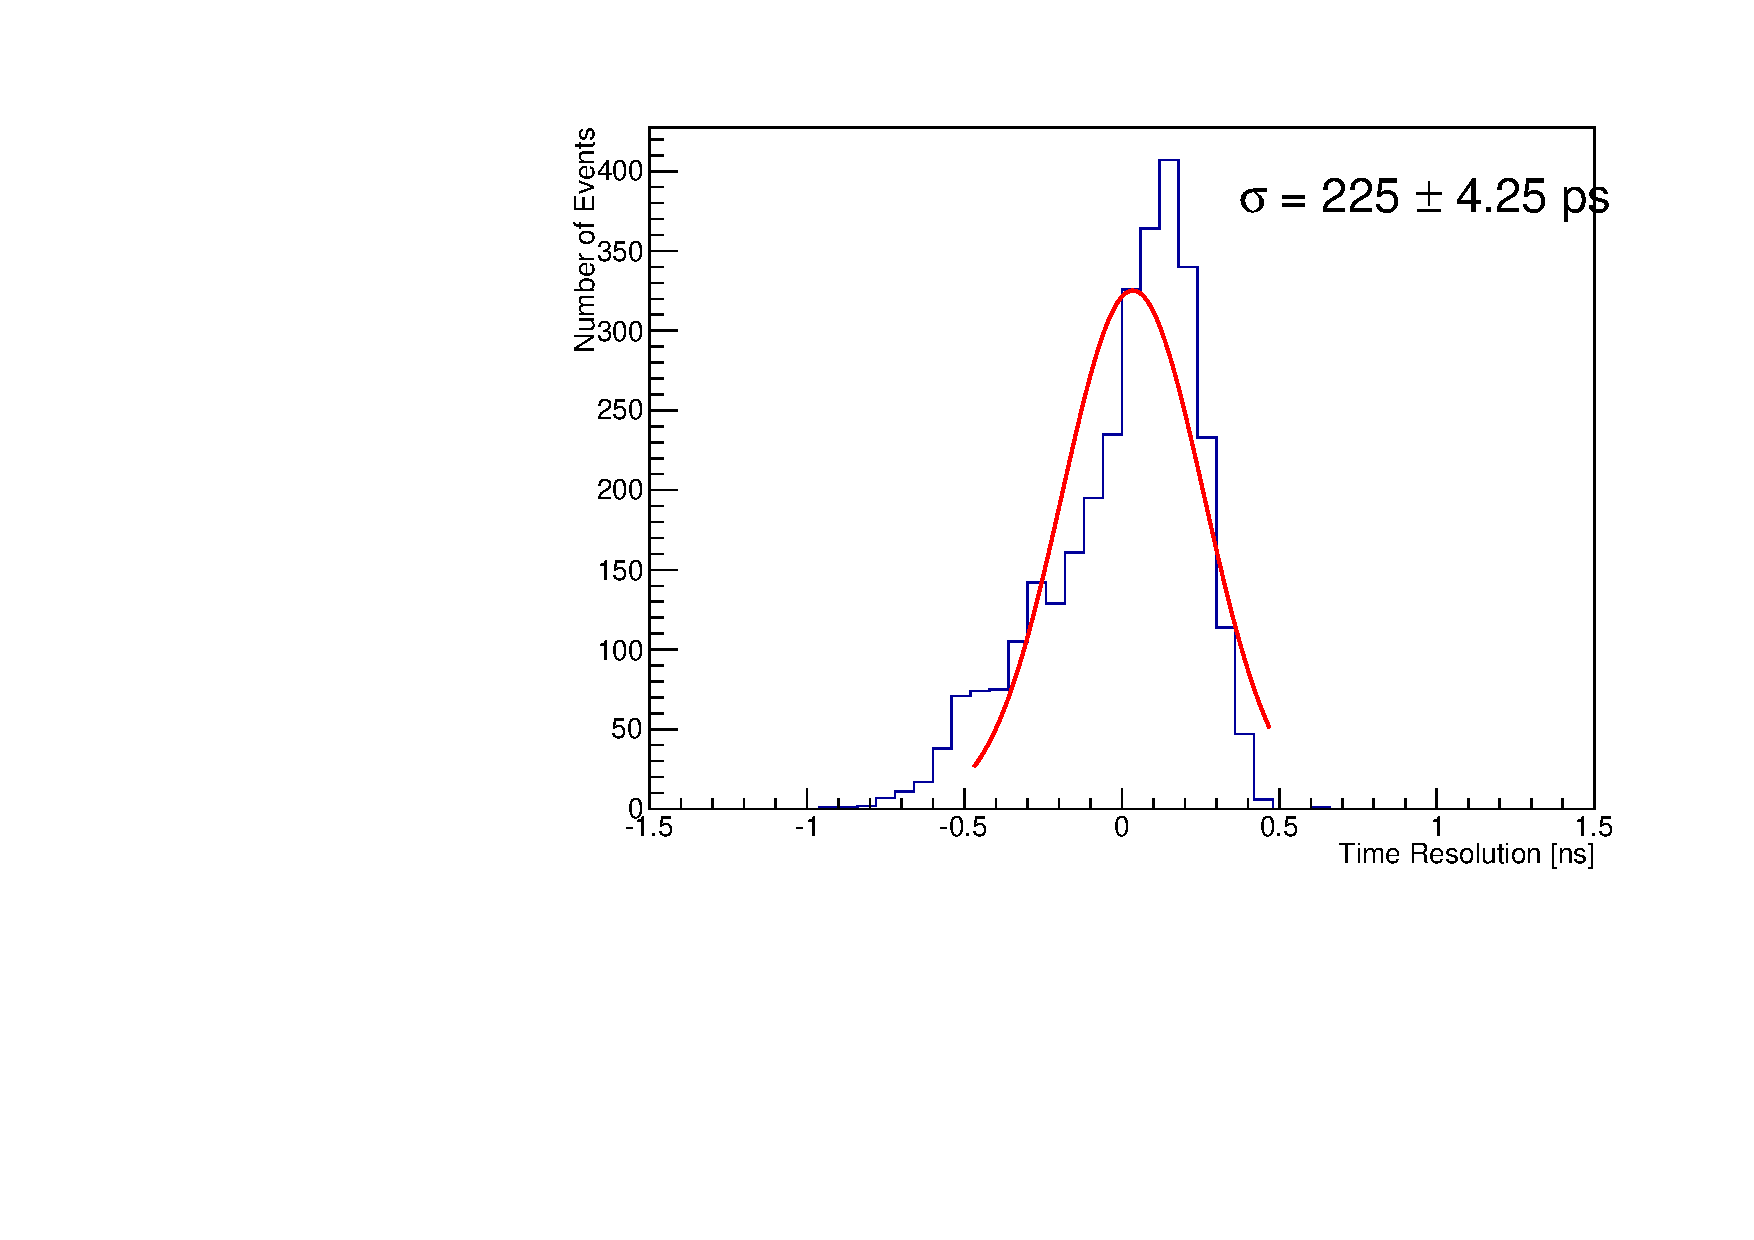
\includegraphics[width=\textwidth]{deltaTSiPad.pdf}
	\caption{TOF of the Silicon Pad}
	\label{fig:SiPad}
\end{minipage} \hfill
\begin{minipage}[t]{.49\textwidth}
	\centering
	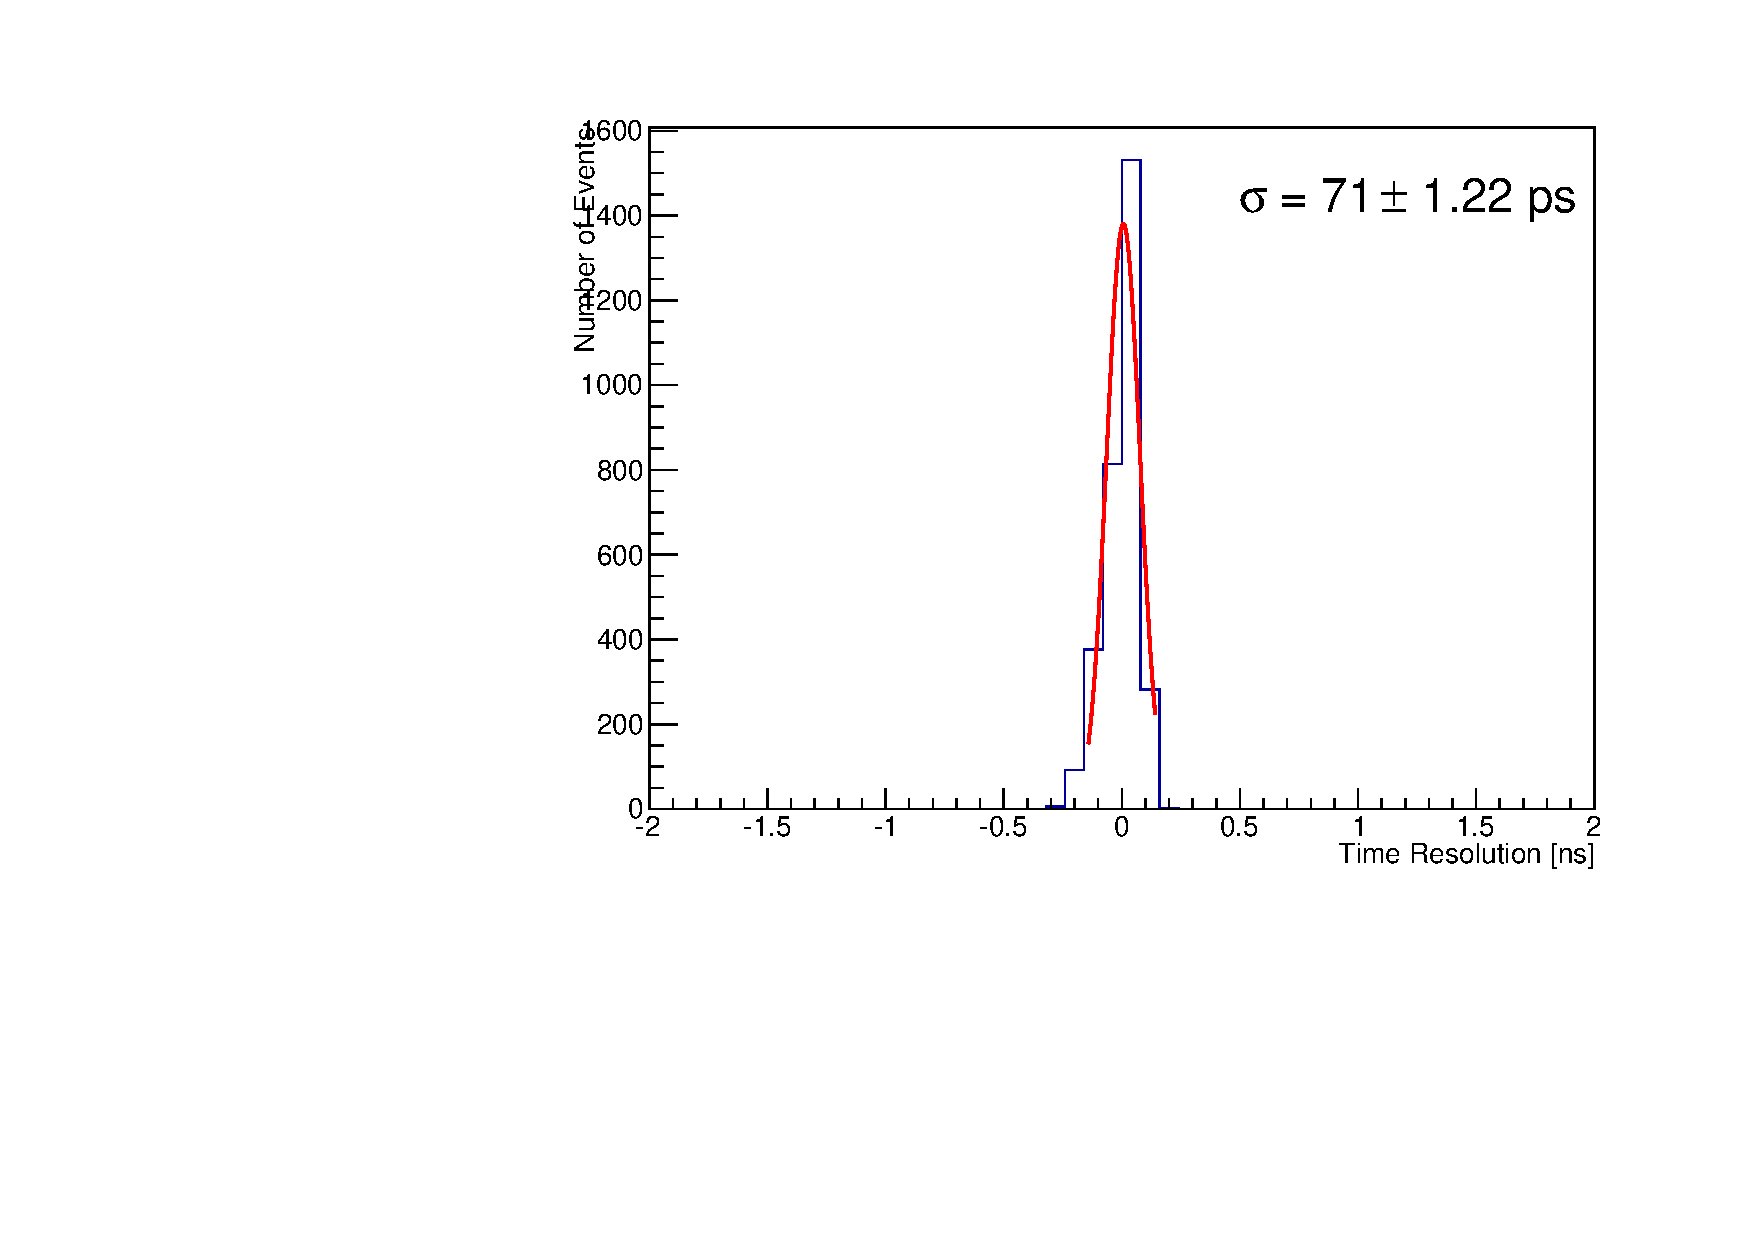
\includegraphics[width=\textwidth]{deltaTWeightsCorrected_totalcharge.pdf}
	\caption{TOF of the HGC Center Pixel, Photonis, and Silicon Pad Combined with Total Device Charge Weighting}
	\label{fig:wctc}
\end{minipage}
\end{figure}


\subsection{Data Analysis: Event Selection}
Before discussing the various ways to combine the $\Delta t$ values from different detectors, the methodology for selecting events that contribute to their individual TOF histograms should be reviewed.
Because not every event contains a detected pulse, and some have a lot of ringing noise and a small signal-to-noise ratio, some events need to be cut out of the $\Delta t$ calculations. 
In order to ensure that most of the \textit{"bad"} events are removed from the histograms, a cut is applied to the calculated peak amplitude (in mA) and to the overall charge (in pC) of the event in that detector, forcing them both to be higher than some threshold. 
This requires that the peak found is not just noise and that the charge (found by integrating the plot) is significant enough to represent a pulse.

For example, analyzing the data (with \textit{dat2rootCP}) from runs 65-83 returns a maximum amplitude value in the Photek for every event. 
Filling a histogram with all of these values in the command-line in ROOT gives the left plot in Figure \ref{fig:AmpCut}. 
Clearly the amplitudes that are near zero or negative are events without pulses or very noisy events. 
These events should be ignored, so a cut is implemented to select for amplitudes above a certain value. 
In this case the value appears to be $0.1\times\sqrt{10}$ mA. 
The right plot in Figure \ref{fig:AmpCut} shows the histogram of the amplitudes with only the events that passed the cut. 
Figure \ref{fig:ChargeCut} shows the same methodology being applied to the charge distribution, with a cut at $2\times\sqrt{10}$ pC. 
Similar cuts were made in the HGC pixels and Photonis MCP. 

\begin{figure}[h]
\centering
	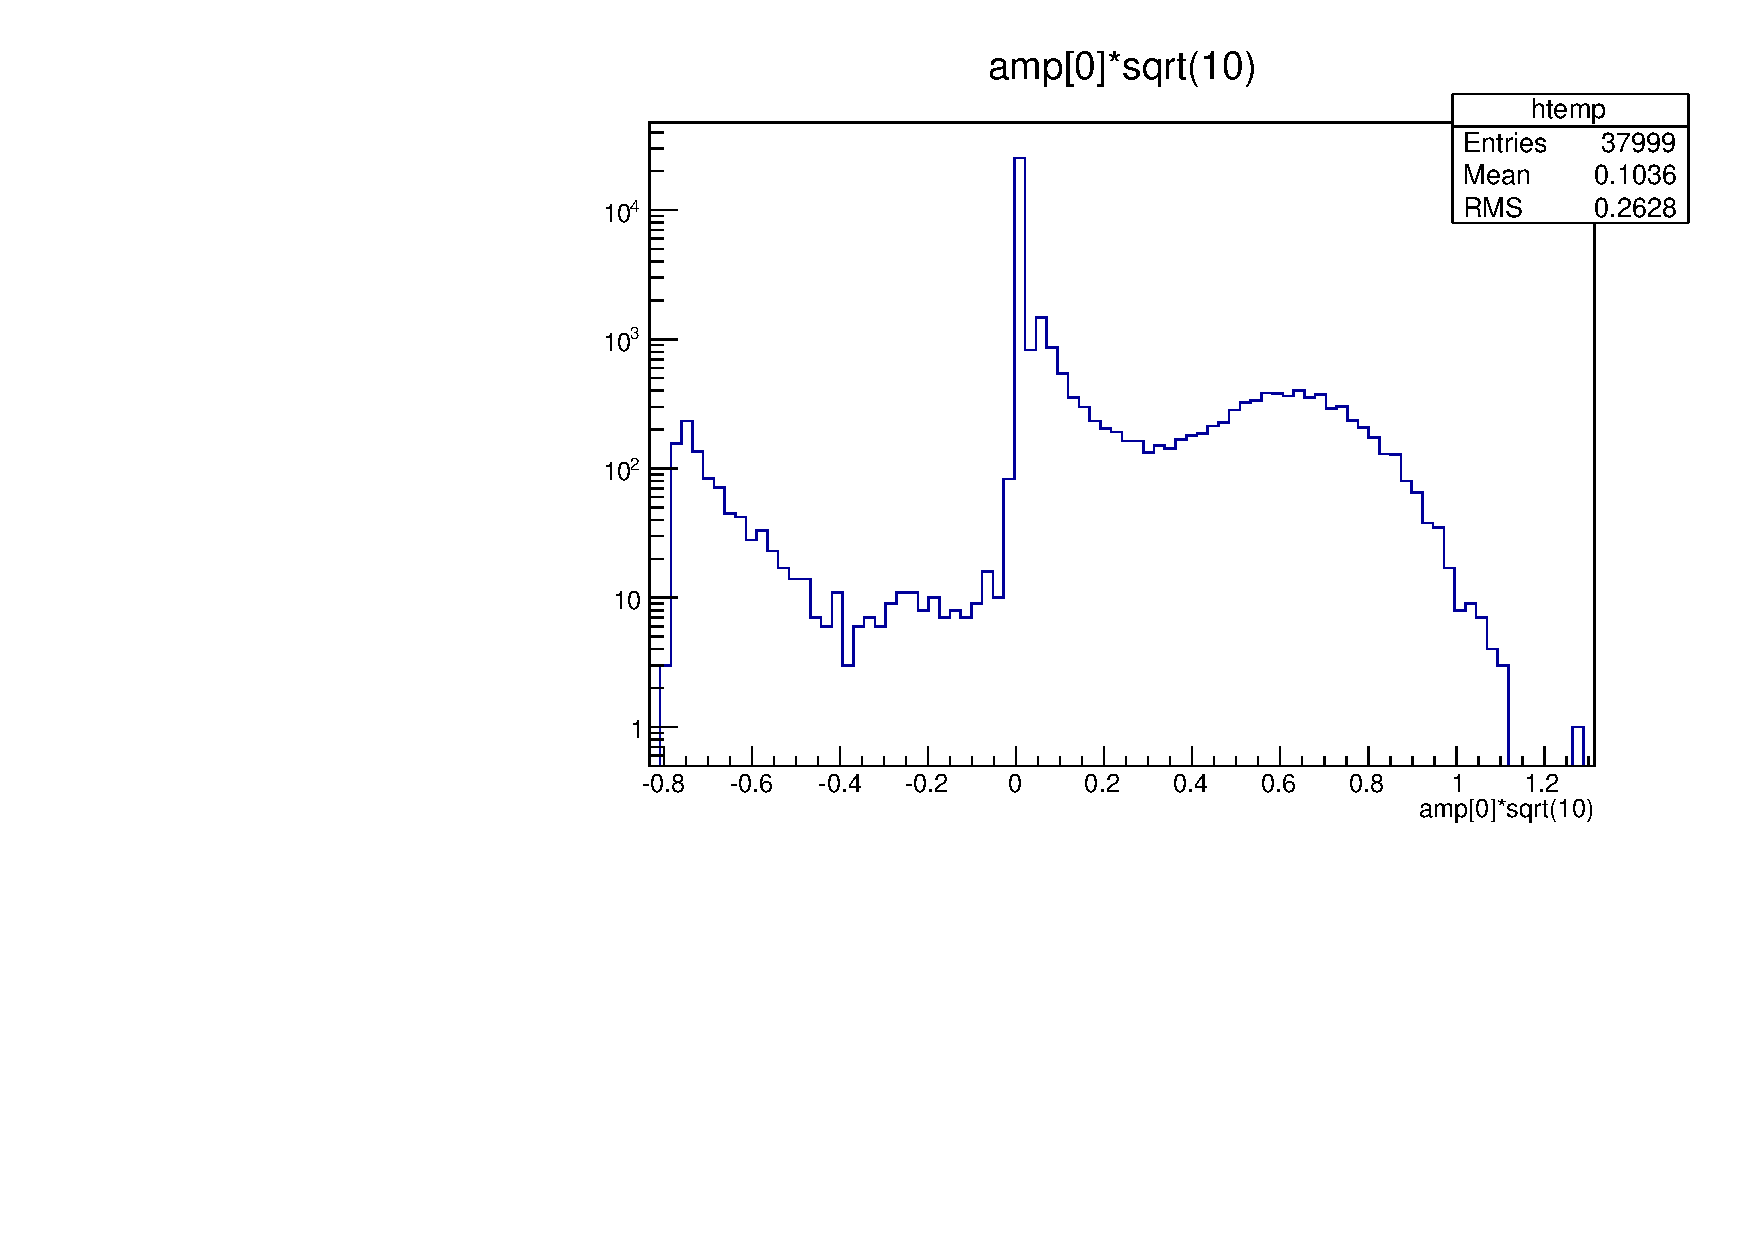
\includegraphics[width=0.49\textwidth]{AmpCut0.pdf}
	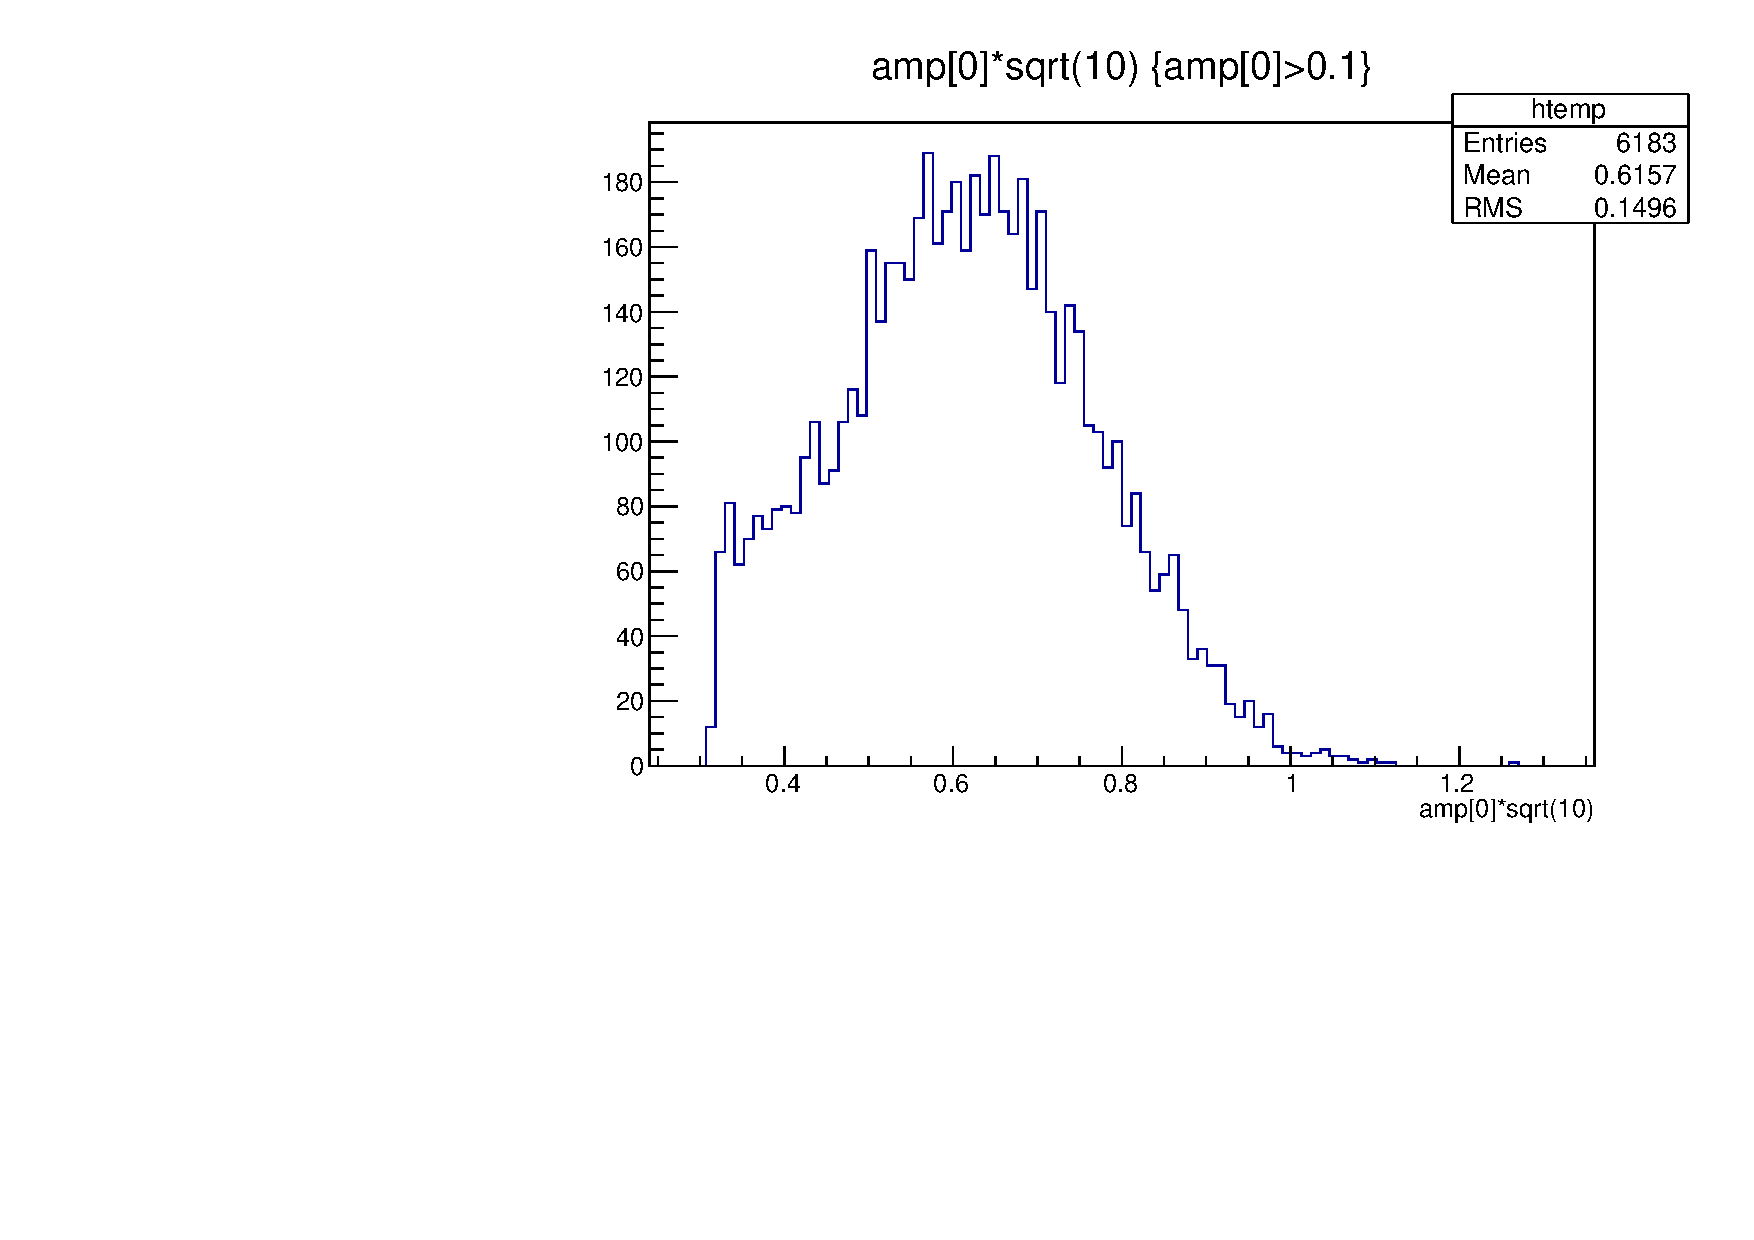
\includegraphics[width=0.49\textwidth]{AmpCut1.pdf}
	\caption{Pulse peak amplitude distribution for the Photek 240 MCP before and after the cut.
		Non-positive amplitudes represent \textit{"bad"} events.
		The $\sqrt{10}$ factor accounts for a 6 dB attenuator.}
	\label{fig:AmpCut}
\end{figure}

\begin{figure}[h]
\centering
	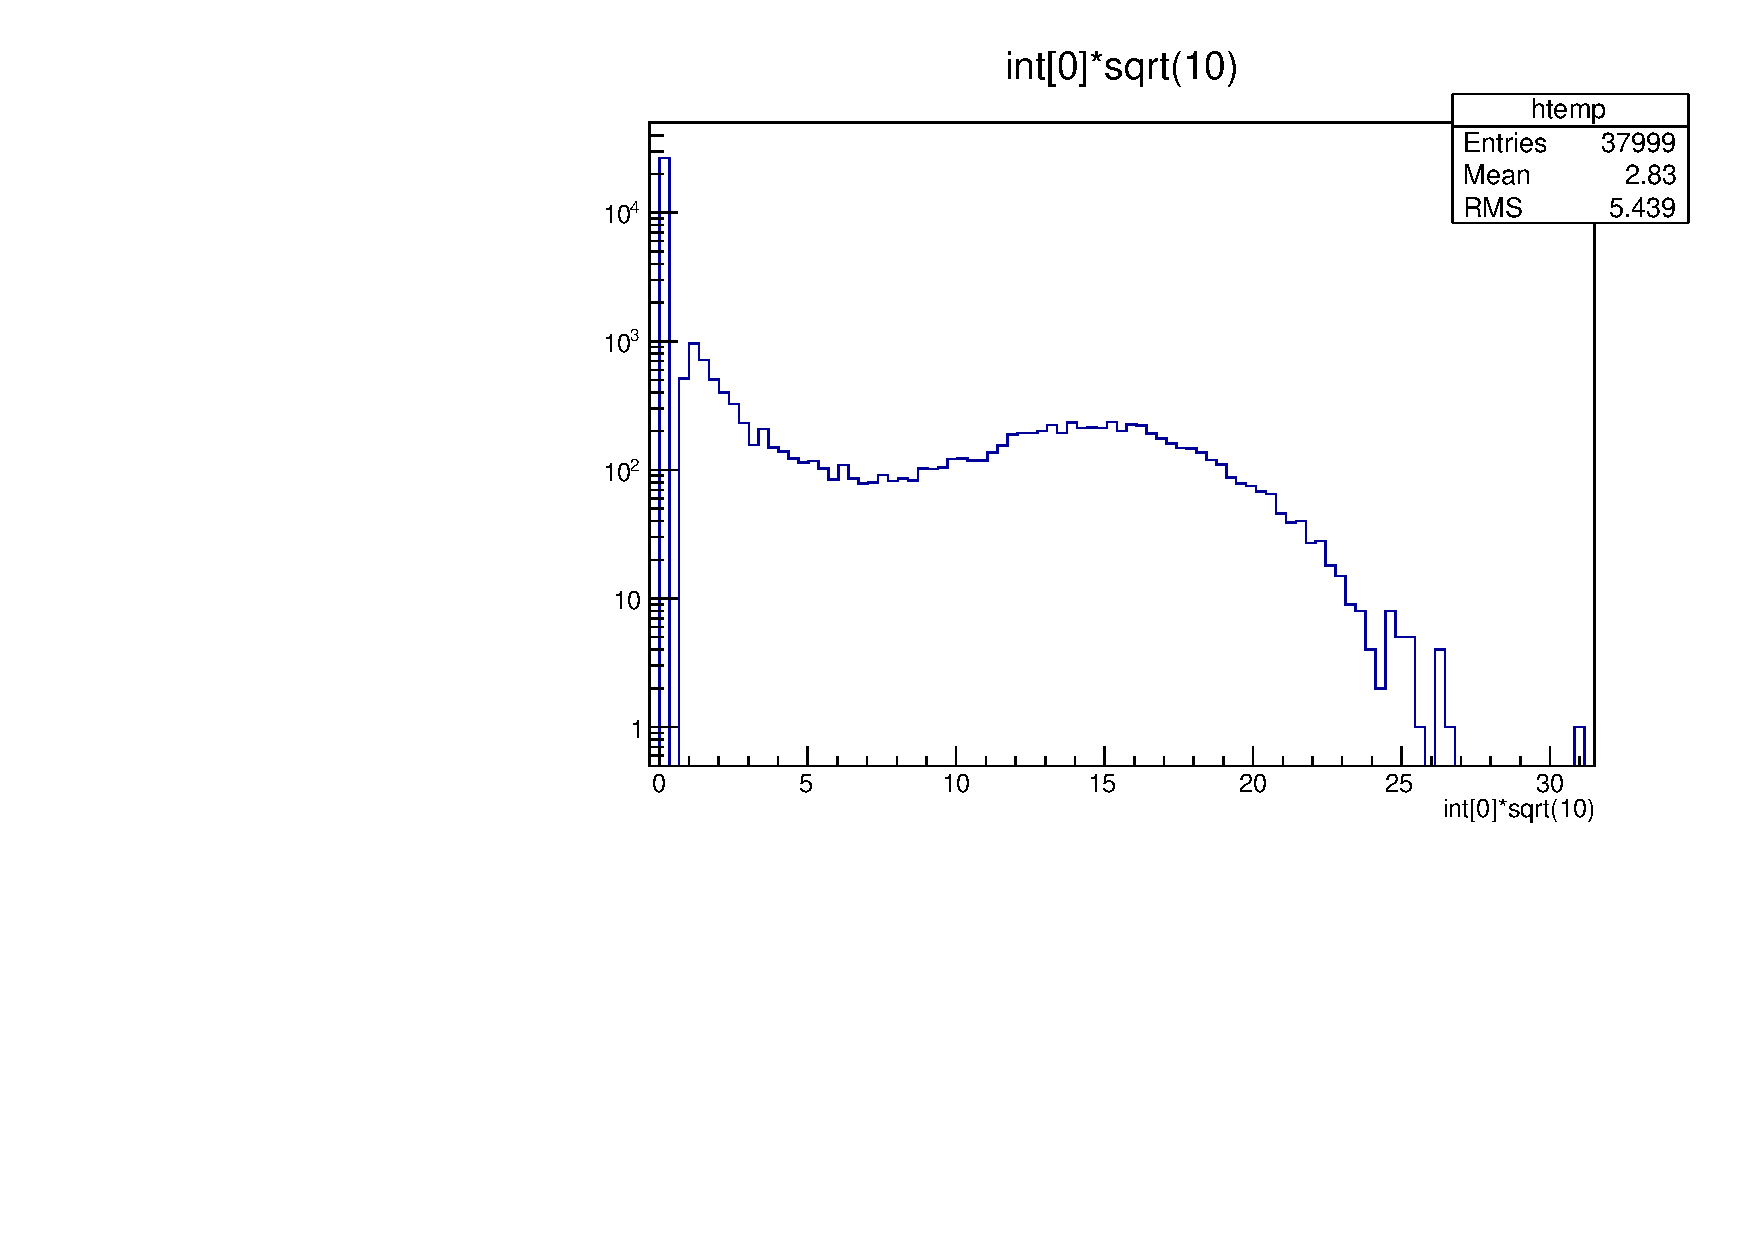
\includegraphics[width=0.49\textwidth]{ChargeCut0.pdf}
	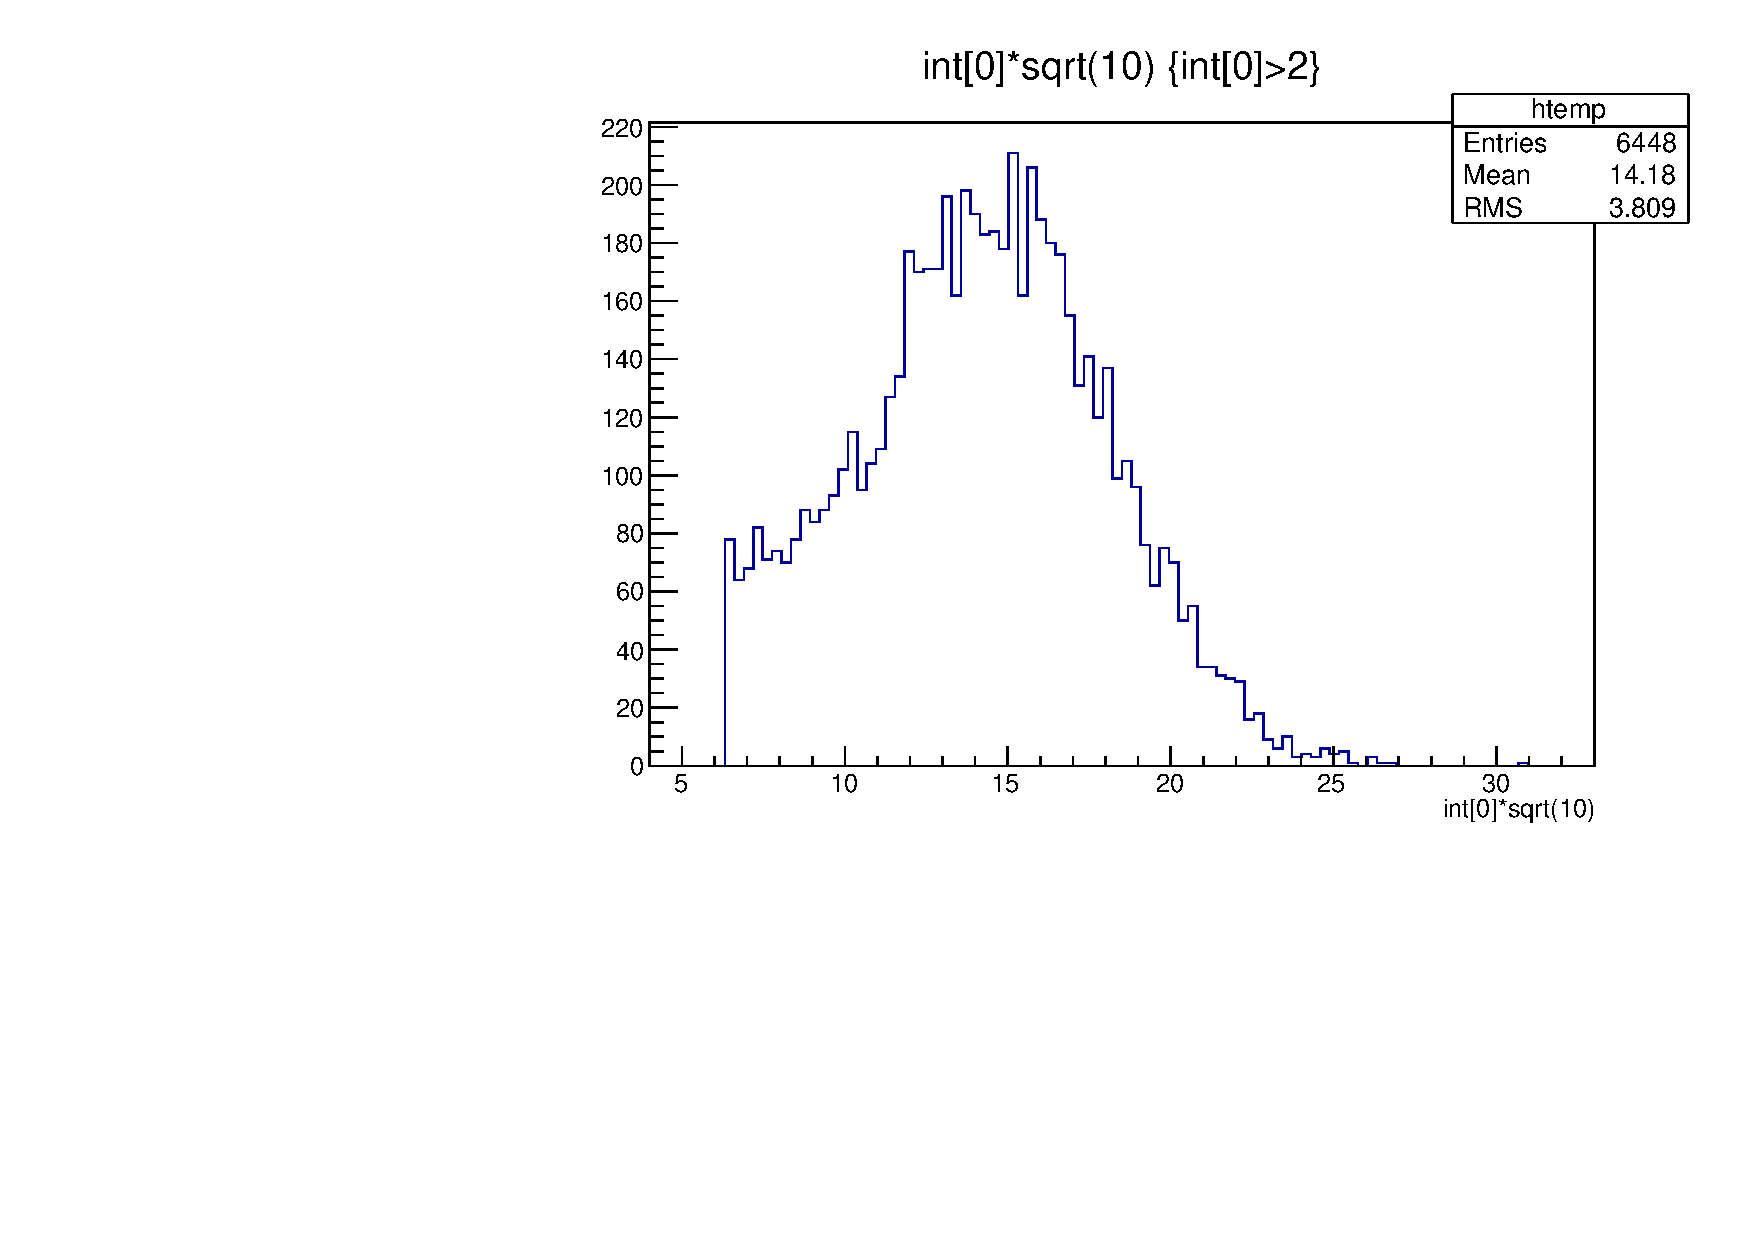
\includegraphics[width=0.49\textwidth]{ChargeCut1.pdf}
	\caption{Pulse charge distribution for the Photek 240 MCP before and after the cut.
		Zeroed charges represent events with only noise.
		The $\sqrt{10}$ factor accounts for a 6 dB attenuator.}
	\label{fig:ChargeCut}
\end{figure}

\subsection{Data Analysis: Device Combination}
The \textit{MultiDeviceStudy\_PicosilMCP} code generates many variations of TOF combination histograms. 
The simplest are the HGC center pixel and the single-channel Photonis MCP histograms (Figures \ref{fig:Center} and \ref{fig:MCP}). 
These TOFs are generated without combining the $\Delta t$ values from multiple detectors. 
There are 4 main ways that have been utilized to combine different detectors.

\subsubsection{Combination Method: Equal Weighting}
This weighting method is the most straightforward. 
If there are 2 devices which all pass the cuts, then their $\Delta t$ values are computed. 
These 2 $\Delta t$ values are then combined into a single $\Delta t$ value by computing the arithmetic average. 
This final $\Delta t$ is then used to populate the histogram. 
Mathematically, this is given by,

\[
\Delta t_{final} =
\dfrac{\Delta t_1 + \Delta t_2}{2} .
\]

It gets slightly harder to compute this $\Delta t_{final}$ when some combinations do not require that \textit{all} detectors pass the cuts, such as when trying to combine the center HGC layer pixel with the 6 inner ring pixels. 
Because many events have 3 or 4 pixels passing cuts, but only a few events have all 7 passing cuts, the $\Delta t_{final}$ is calculated at every event using whichever pixels were able to pass the cuts. 
This means the number of $\Delta t_{initial}$'s will vary with event. 
Mathematically, it can more generally be written:

\[
\Delta t_{final_i} =
\dfrac{\sum\limits_{k=1}^N \Delta t_{k_i}} {N} 
\]

for N detectors passing cuts, where $\Delta t_{k_i}$ represents the $k^{th}$ detector's TOF at event $i$.

\subsubsection{Combination Method: Event Charge Weighting}
This weighting method uses the detected event pulse charge in each device to weight each $\Delta t_{initial}$ value. 
As illustrated in Figure \ref{fig:ChargeCut}, the pulse charge varies with event, so the relative weightings between detectors will change on an event-by-event basis. 
Mathematically, an event's charge weighting is given by,

\[
\Delta t_{final_i} =
\dfrac{\sum\limits_{k=1}^N \Delta t_{k_i} q_{k_i} }
	{\sum\limits_{k=1}^N q_{k_i} }
\]

for N detectors passing cuts, where $q_{k_i}$ represents the $k^{th}$ detector's charge at event $i$.

\subsubsection{Combination Method: Total Charge Weighting}
Whereas the event charge method weights each detector differently for different events, the total charge method weights each detector the same way over the entire run. 
Rather than use the event charge, this method sums a detector's event charge for every event in the run, and uses that value as the weighting factor. 
Mathematically,

\[
\Delta t_{final_i} =
\dfrac{\sum\limits_{k=1}^N \Delta t_{k_i} Q_k }
	{\sum\limits_{k=1}^N Q_k }
,\ \ \ \ 
Q_k = \sum_{all\ events\ i} q_{k_i}
\]

for N detectors passing cuts, where $q_{k_i}$ represents the $k^{th}$ detector's charge at event $i$.

\subsubsection{Combination Method: Charge MPV Weighting}
Like the total charge method, this method also assigns weighting factors to each detector that do not change with the event. 
This method is additionally only used within the HGC layer, for combining the TOFs of different pixels. 
Rather than being determined by the total charge detected, this method fits a Landau distribution to the charge distribution histogram of each of the inner ring pixels.
The peak -- most probable value (MPV) -- of the fit is then used as the weighting factor for the inner ring pixels. 
Because there are far more events passing cuts -- and with a higher charge -- in the center pixel, the distribution is Gaussian, and its weighting factor is the mean of a Gaussian fit.
Both types of fits are accomplished by maximizing the log-likelihood in order to avoid the biasing of the $\chi^2$ minimization fit for low-event bins.
Mathematically, this method is represented by the same formula as the total charge method, letting $Q_k$ represent the detector's MPV, instead of total charge.

\section{Time of Flight Plots: Simple Combinations}
Now that all the different combination methods have been described, understanding the resultant plots is now possible. 
In order to show results in the simplest manner, this section will only use plots coming from 1 data set with the same configuration. 
Specifically, the results in this section will all be for runs 104-116 excluding runs 111-114, which have a test beam of 32 GeV electrons, and a tungsten (W) absorber 1mm in front of the HGC layer (it may help to recall the setup from Figure \ref{fig:setup}).

Starting from the lower-level plots, Figure \ref{fig:center_MCP_104} contains the TOF histograms for the HGC center pixel and Photonis MCP.

\begin{figure}%[h]
\centering
	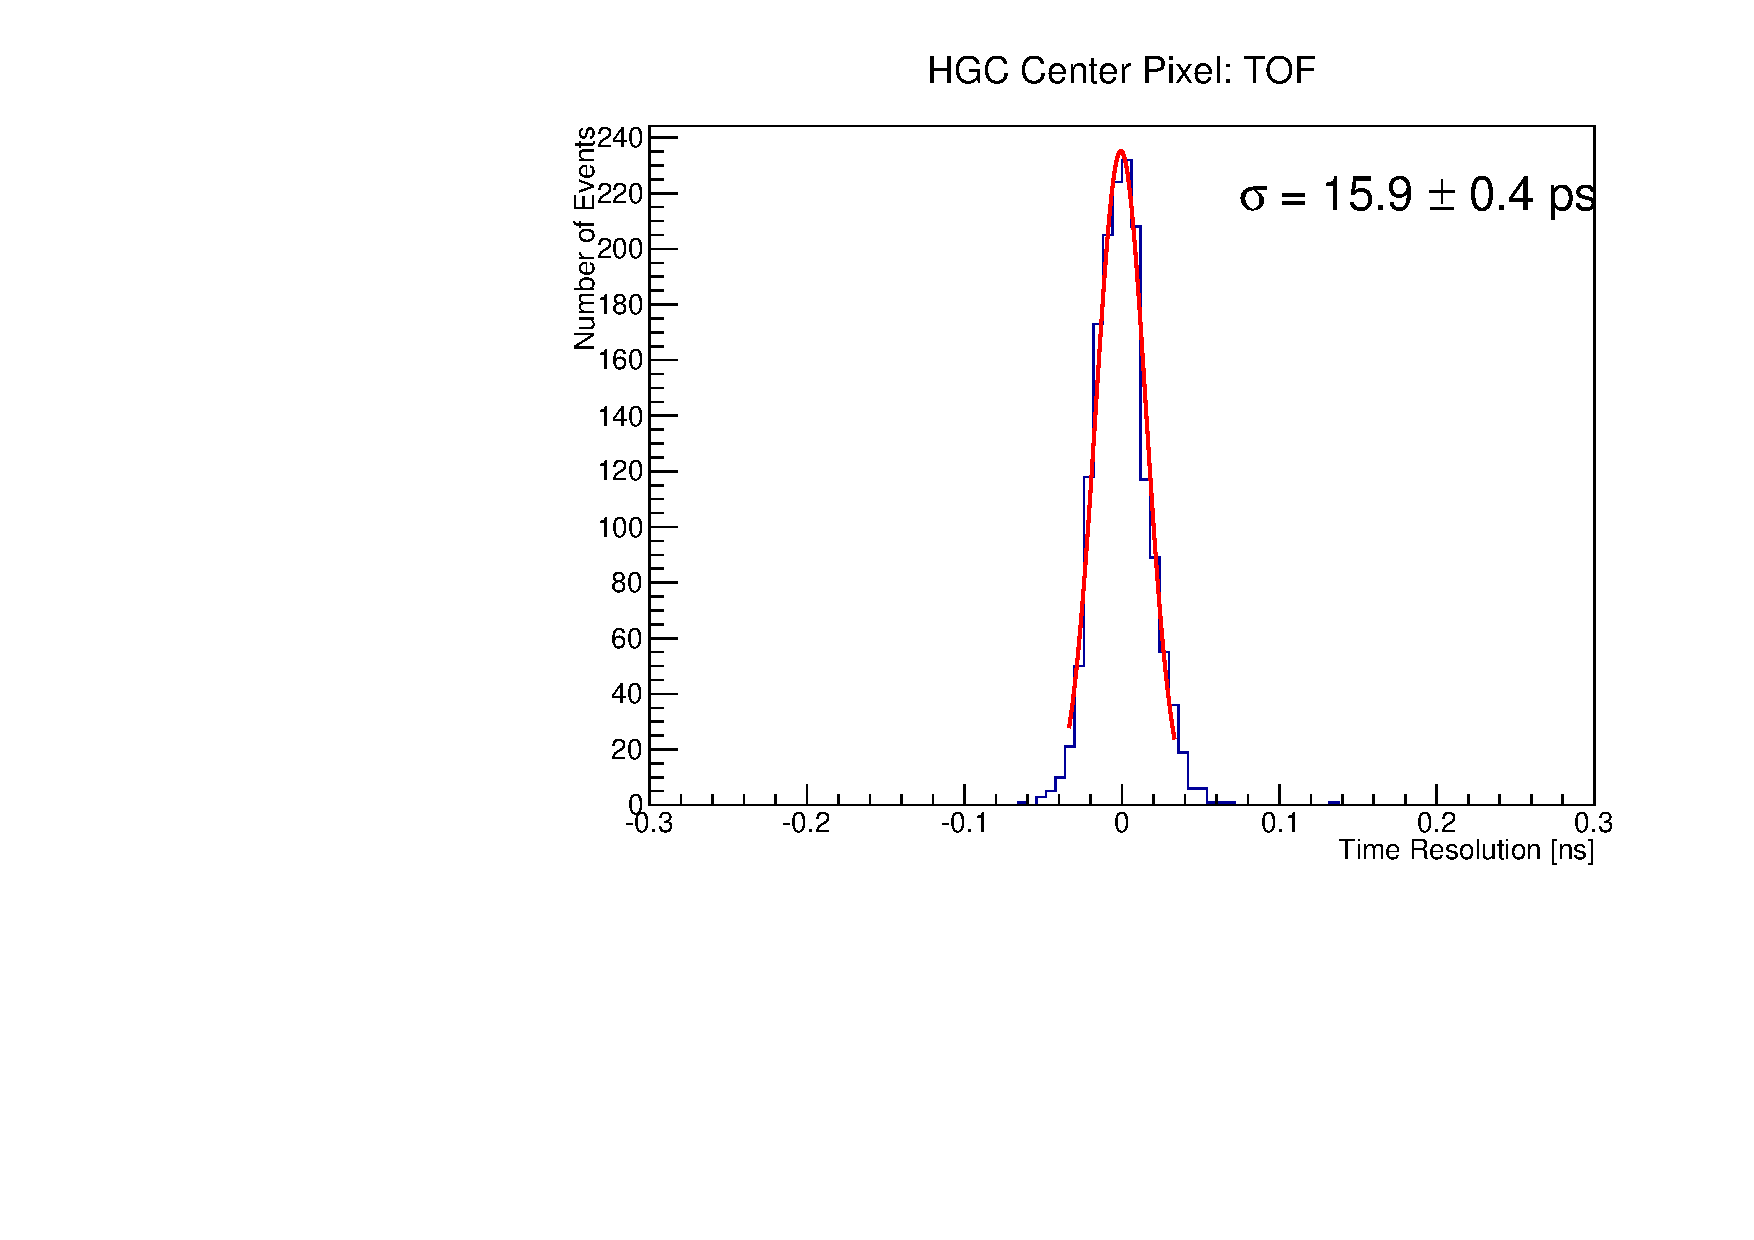
\includegraphics[width=.49\textwidth]{deltaTCenter104.pdf}
	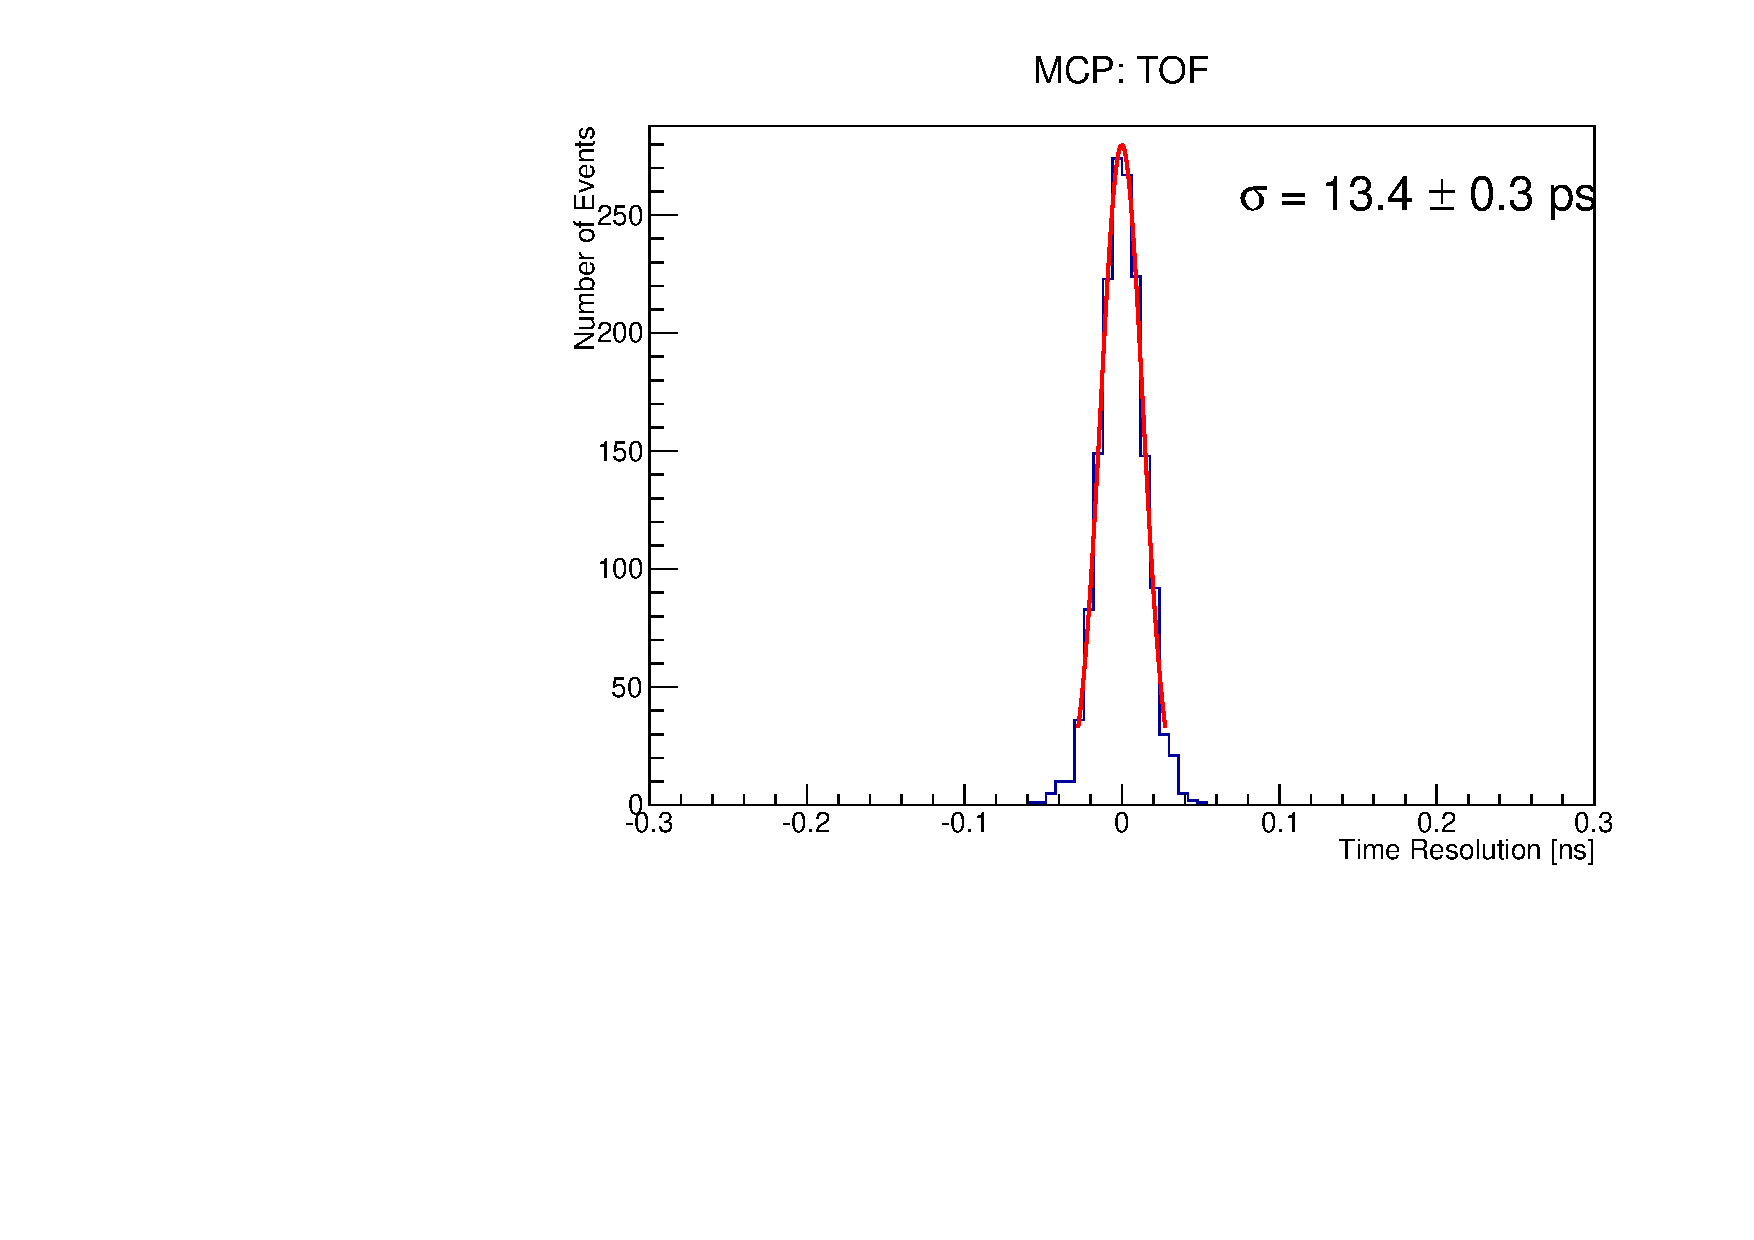
\includegraphics[width=.49\textwidth]{deltaTMCP104.pdf}
	\caption{TOF histograms of HGC center pixel and of Photonis MCP.}
	\label{fig:center_MCP_104}
\end{figure}

In order to see how the time resolution improves when adding in the inner ring pixels, Figure \ref{fig:HGC_event_total_MPV_104} contains different weighting methods based on the charge. 
Equal weighting is not used here because the center pixel has more events and a better resolution than the other pixels, so it should be weighted more heavily. 
In Figure \ref{fig:HGC_event_total_MPV_104}, there is a decrease in $\sigma$ (from 15.9 ps in Figure \ref{fig:center_MCP_104}) and thus an improvement in the time resolution for all combinations. 
Although the uncertainties in $\sigma$ are too large to be conclusive, Figure \ref{fig:HGC_event_total_MPV_104} suggests that the event charge weighting is the worst of the 3 methods.

\begin{figure}[h]
\centering
	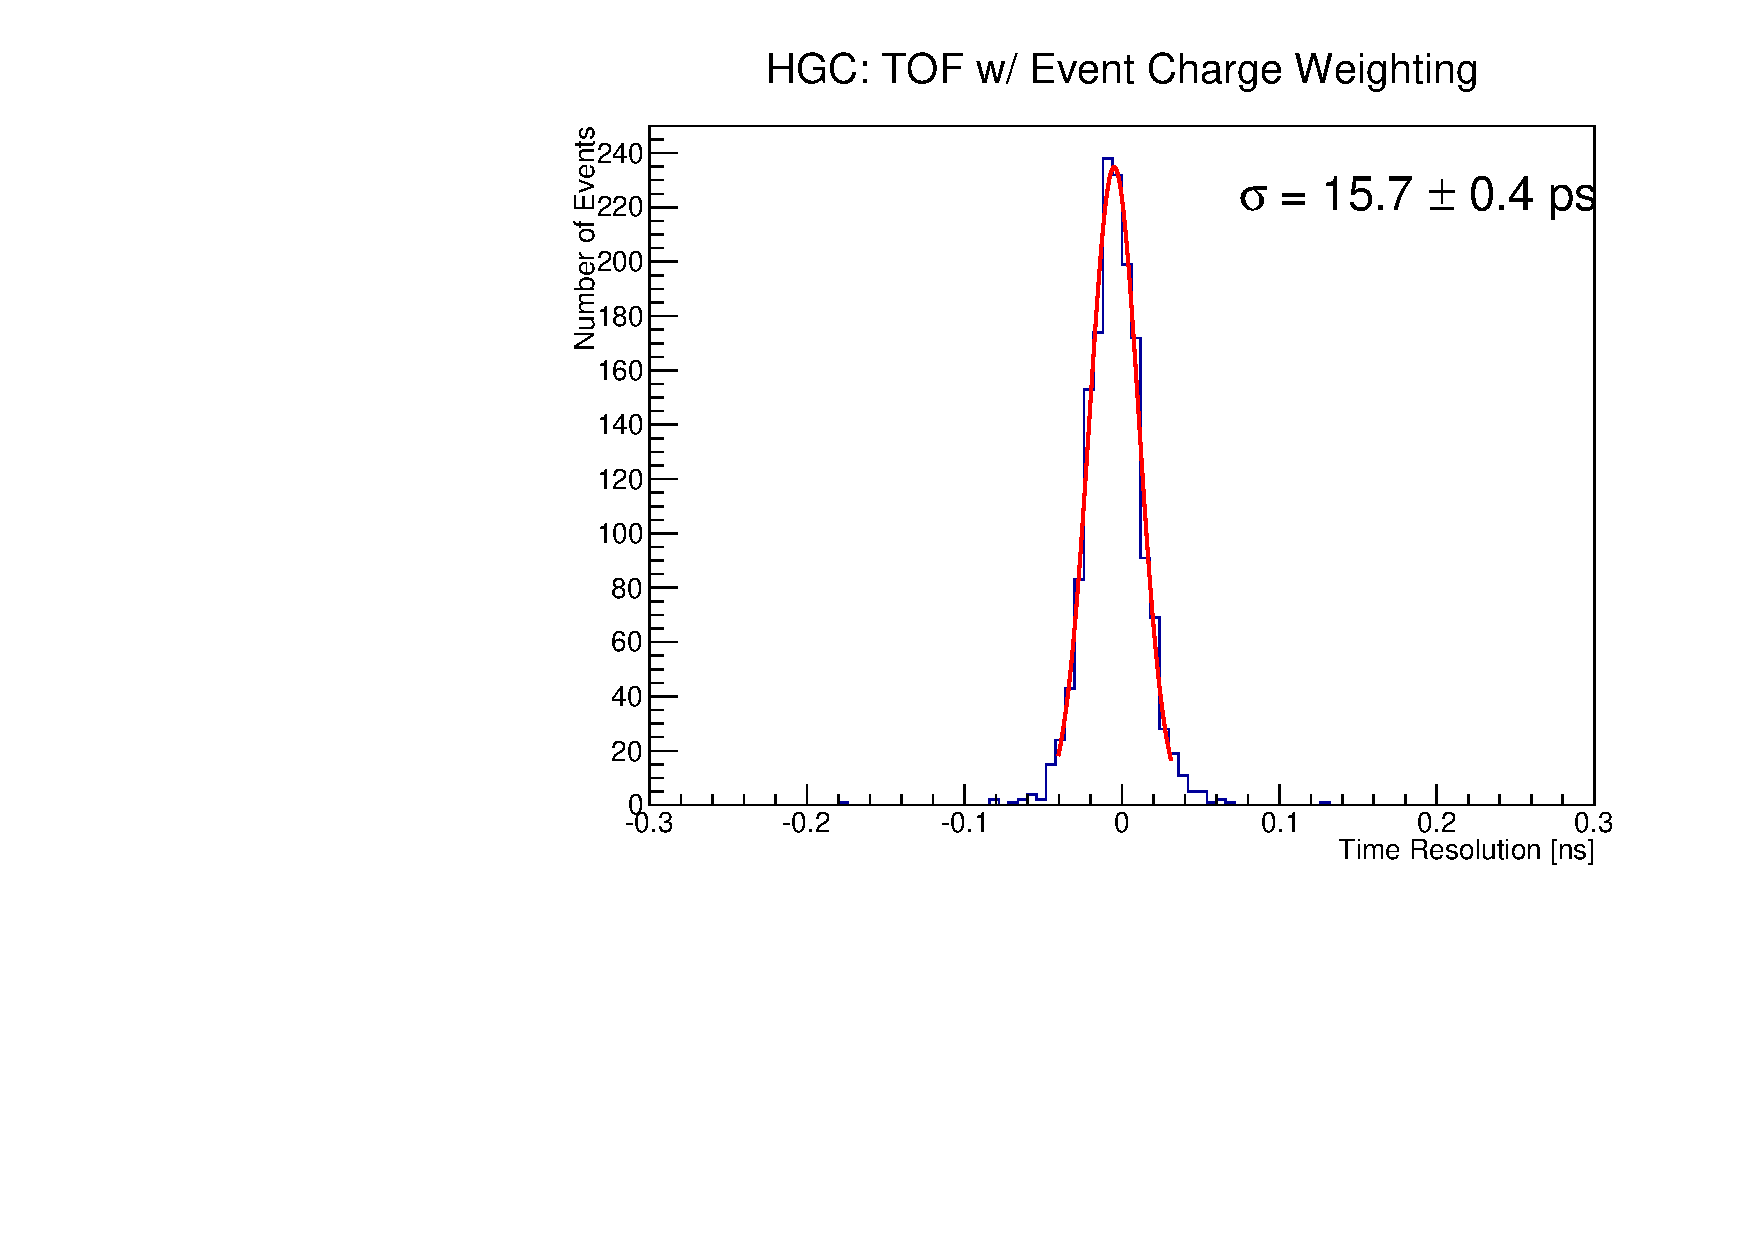
\includegraphics[width=.32\textwidth]{deltaTPicoSilEventCharge104.pdf}
	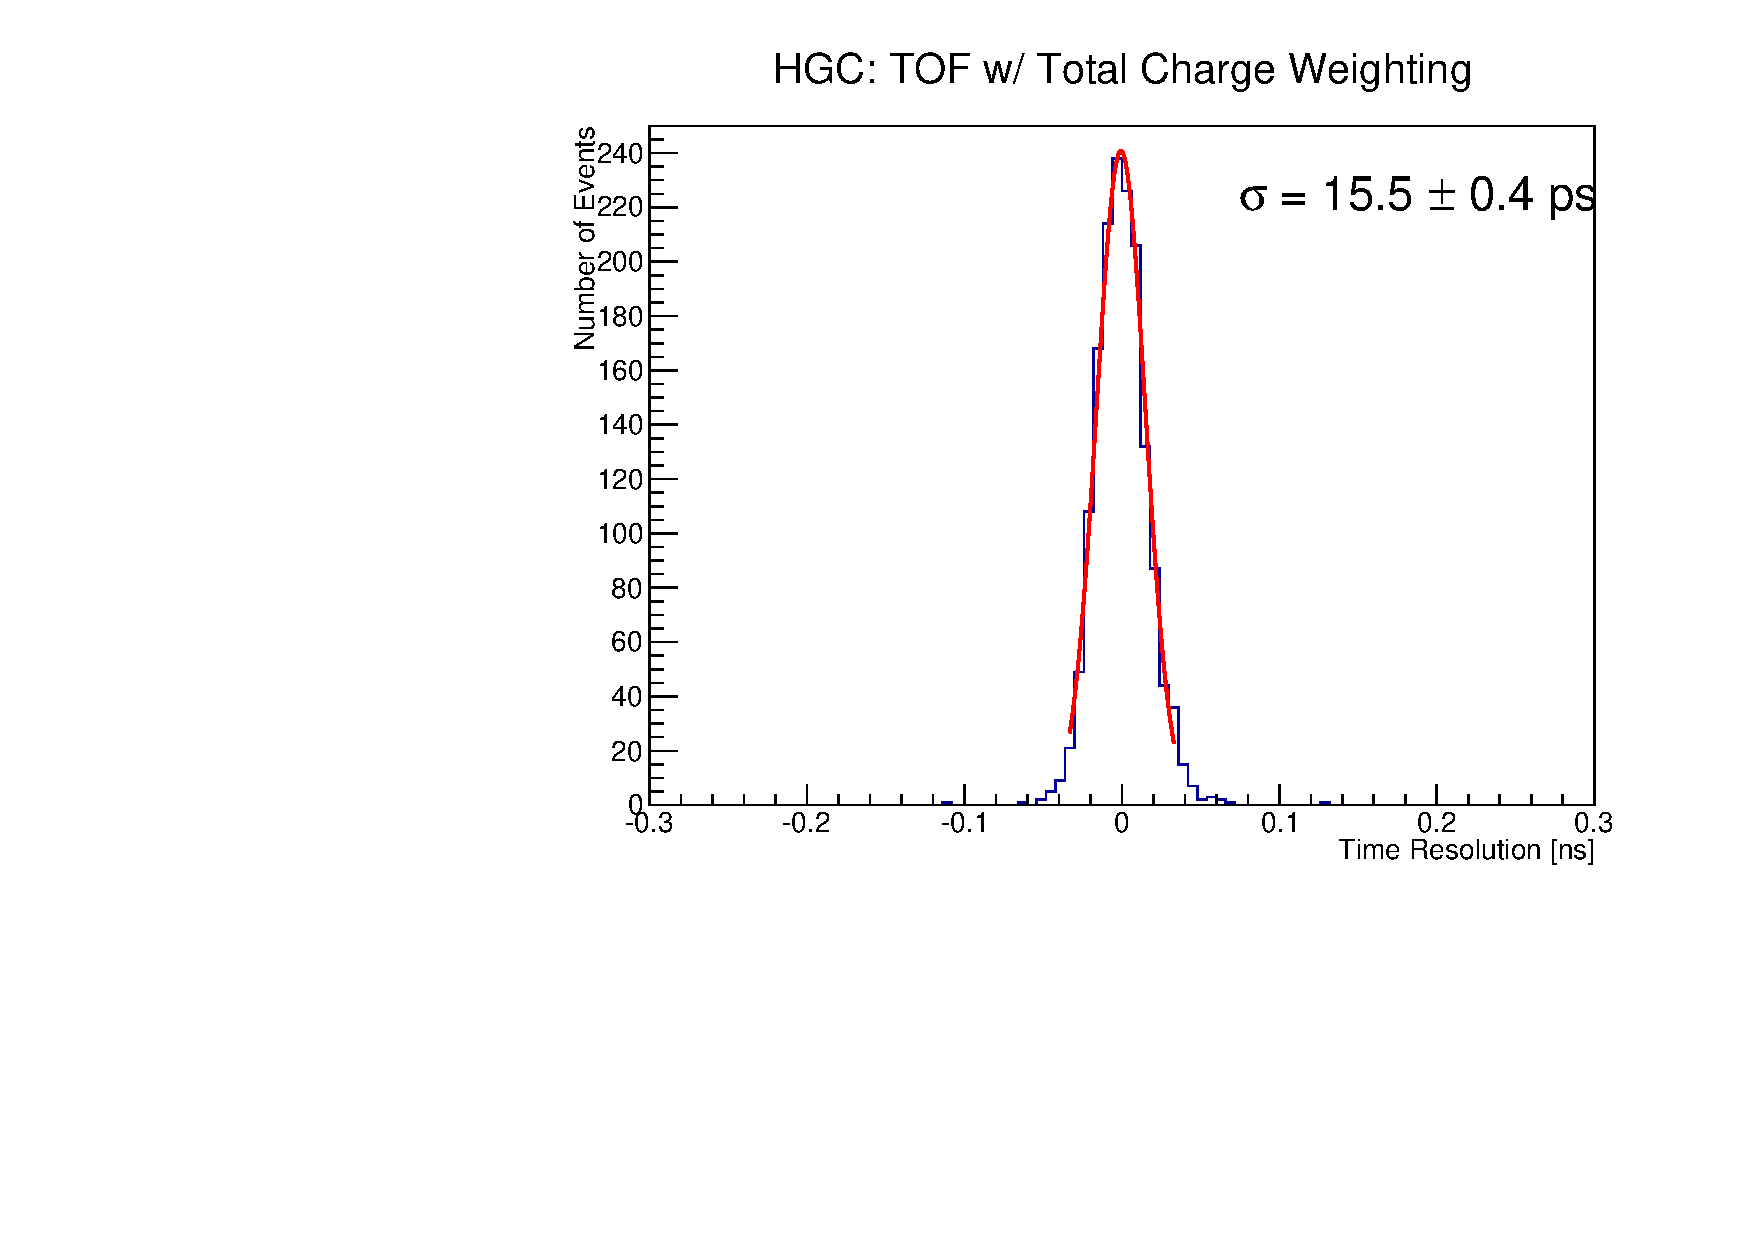
\includegraphics[width=.32\textwidth]{deltaTPicoSilTotalCharge104.pdf}
	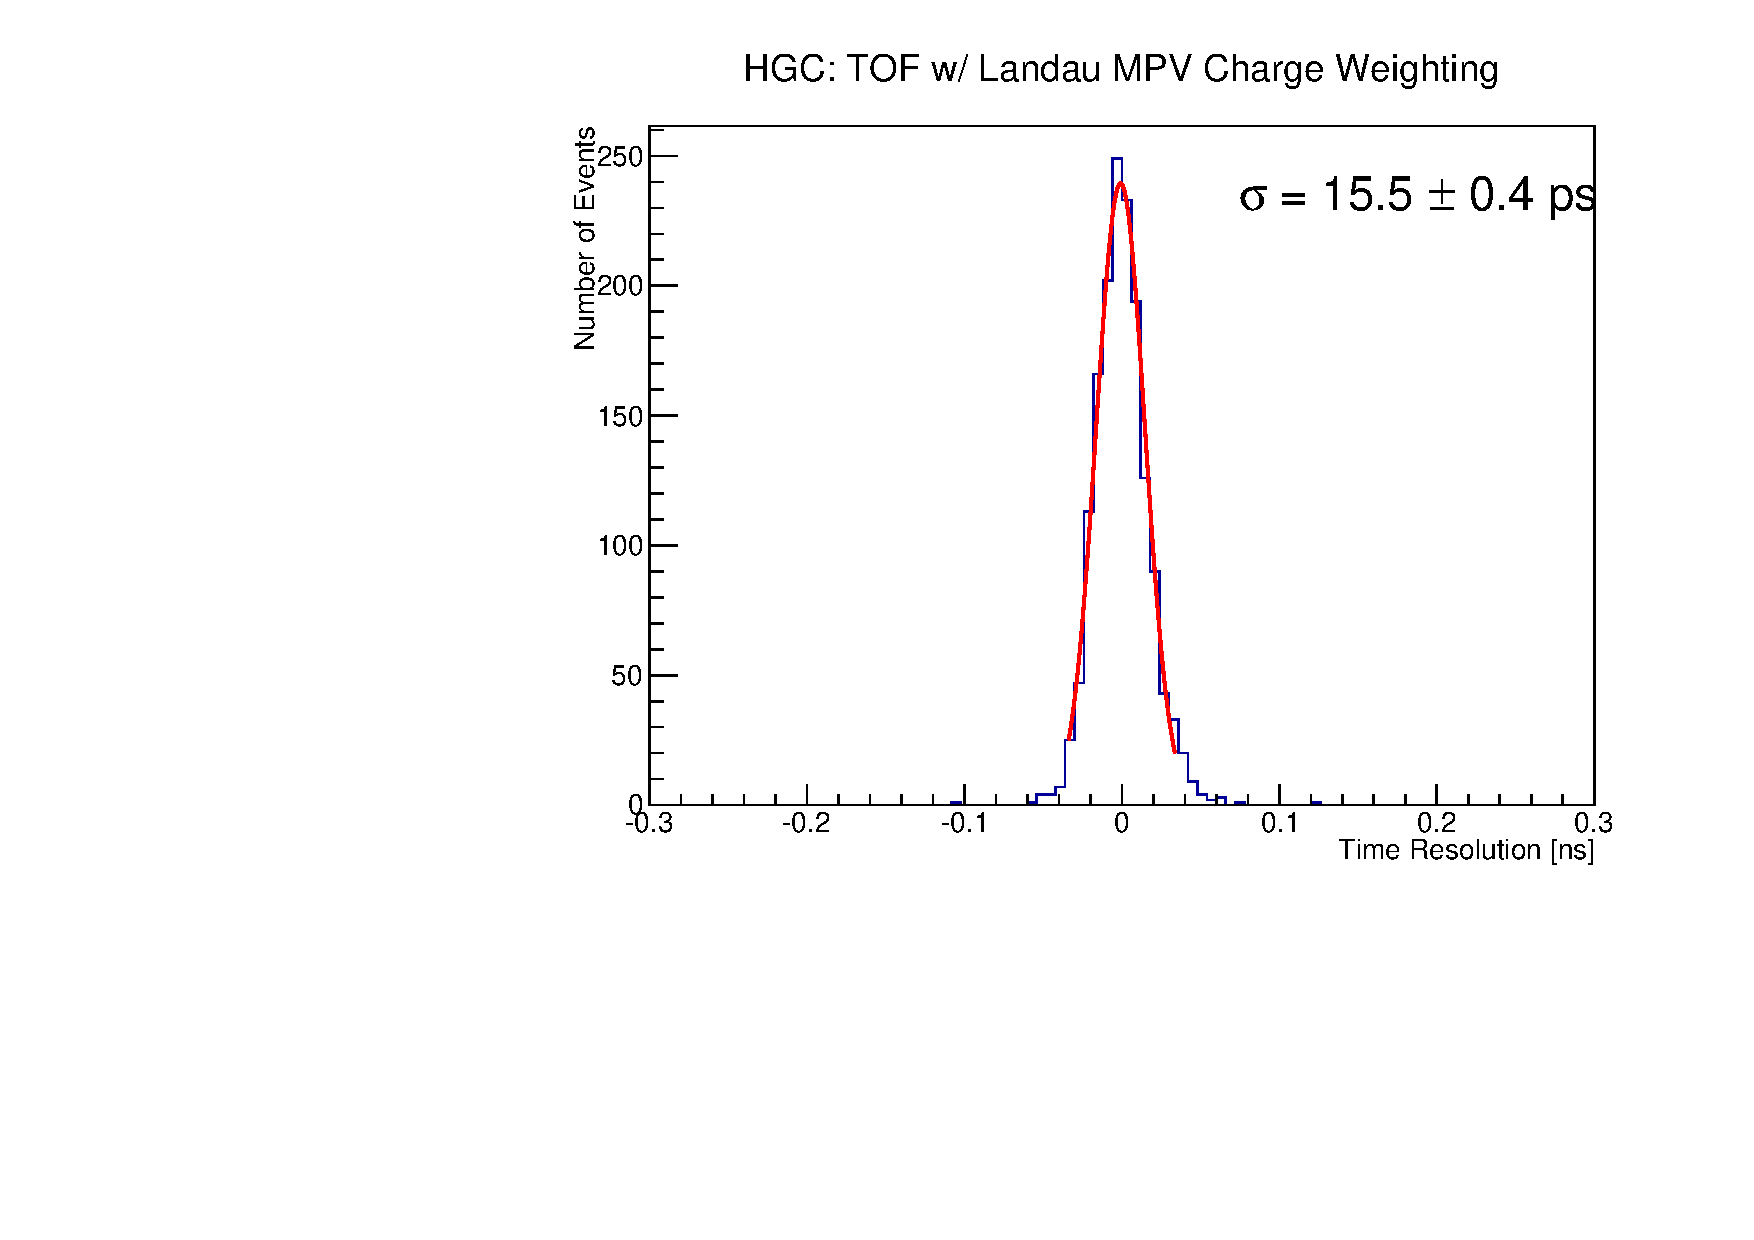
\includegraphics[width=.32\textwidth]{deltaTPicoSilLandauCharge104.pdf}
	\caption{TOF histograms of HGC pixels combined by event charge, total charge, and charge MPV.}
	\label{fig:HGC_event_total_MPV_104}
\end{figure}

The above illustrates the transverse portion of this analysis. 
For the longitudinal aspect, the $\Delta t$ values that are used to populate the HGC layer histograms in Figure \ref{fig:HGC_event_total_MPV_104} will be combined with the Photonis MCP $\Delta t$ values used to populate the right histogram in Figure \ref{fig:center_MCP_104}.
There are some basic and naive ways to combine the HGC layer with the Photonis MCP.
The first method includes assigning an equal weighting to every pixel/detector that passes the cuts.
The second method includes assigning an equal weight to all HGC pixels that pass the cuts and calculating the HGC $\Delta t$, which is then weighted equally with the Photonis $\Delta t$.
This second method can be written mathematically,

\[
\Delta t_i = \dfrac{ \Delta t_{MCP_i} }{2} + \dfrac{\sum\limits_{j=1}^N \Delta t_{HGC_{ij}} }{2\times N},\ \ \ event\ i,\ \ N\ HGC\ pixels\ passing\ cuts.
\]

The results form these two methods can be seen in Figure \ref{fig:m12}. 
Note that these two methods may seem too elementary -- especially the first method, which weights the inner ring pixels too much, and the center pixel and Photonis too little -- but they are brought up now because one of them will be used later in a smarter way. 
Here however, both methods (utilizing 8 detectors) gave a worse time resolution than just the central HGC pixel.	

\begin{figure}[h]
\centering
	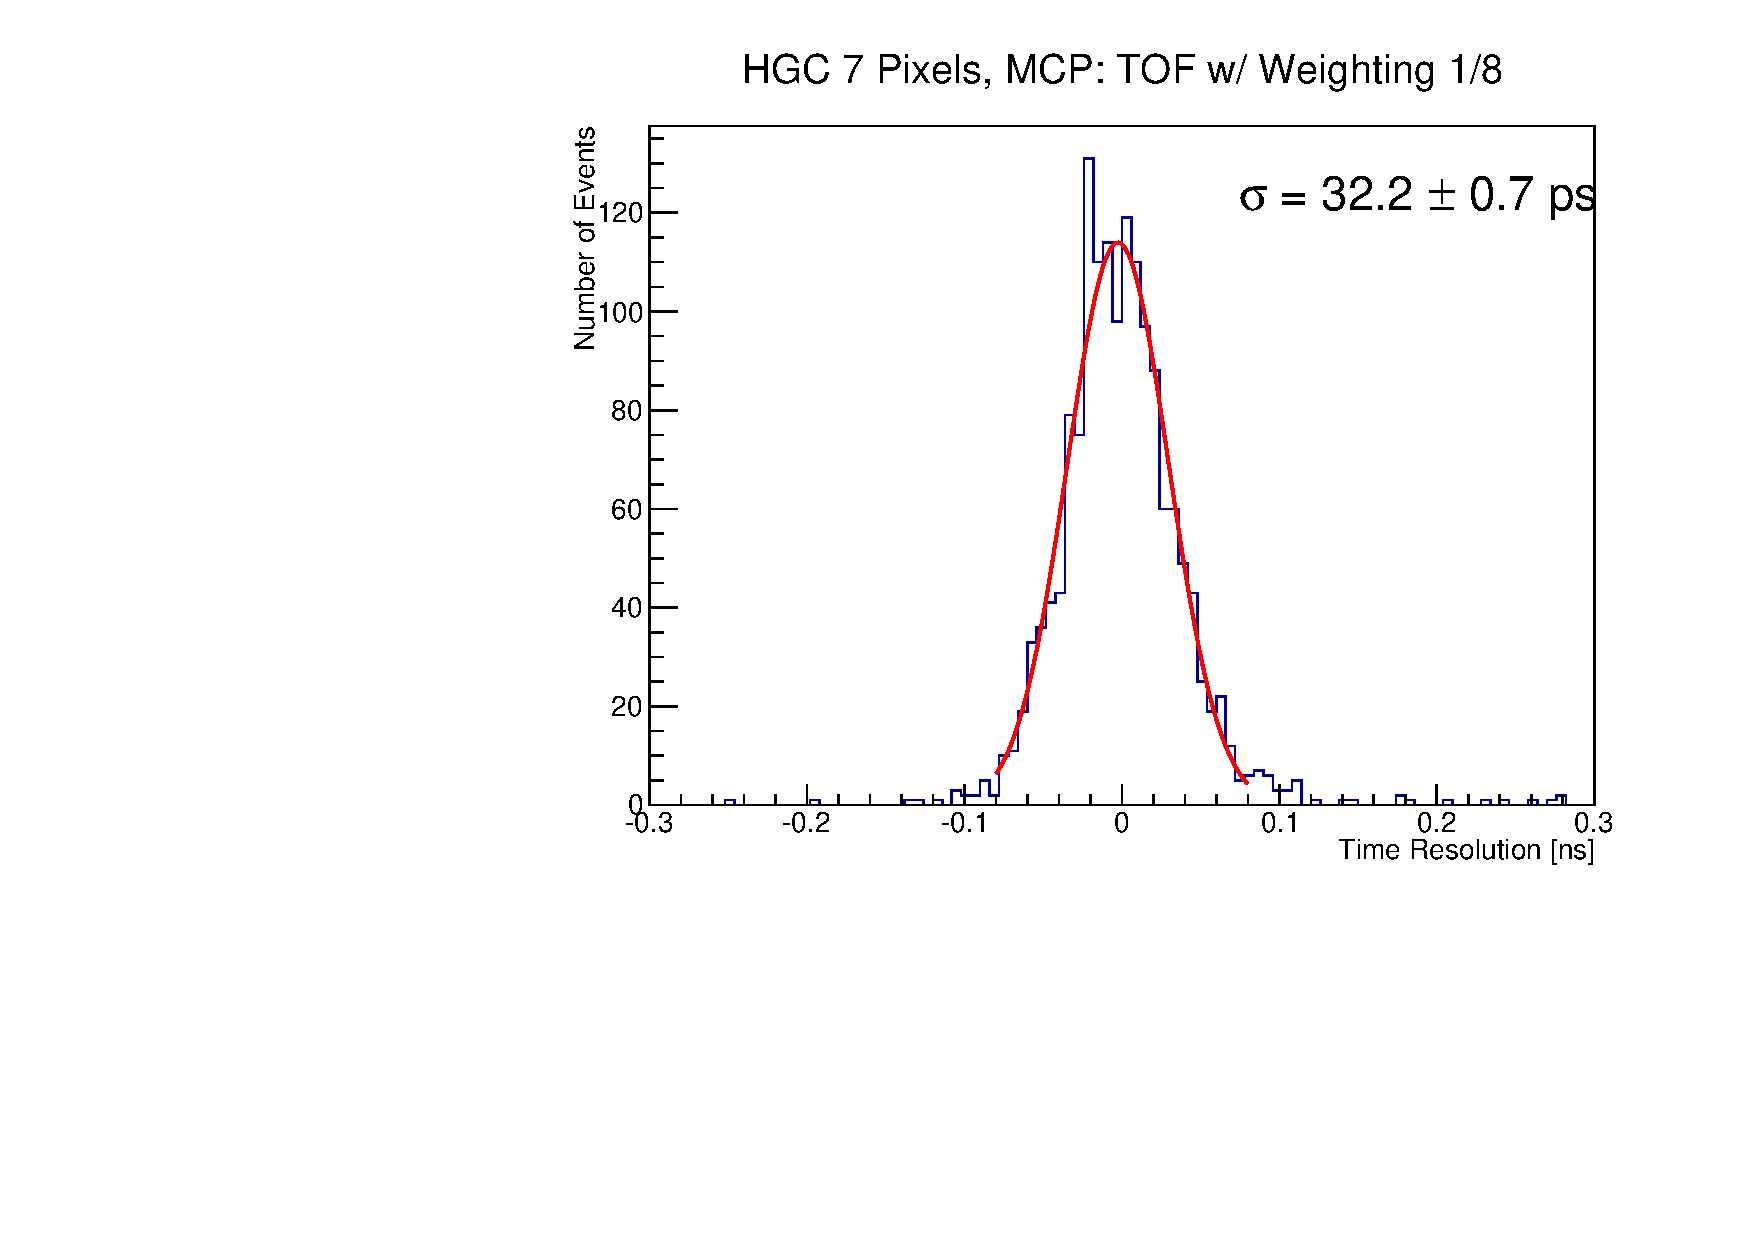
\includegraphics[width=.49\textwidth]{deltaT_PicoSil_MCP_Equal104.pdf}
	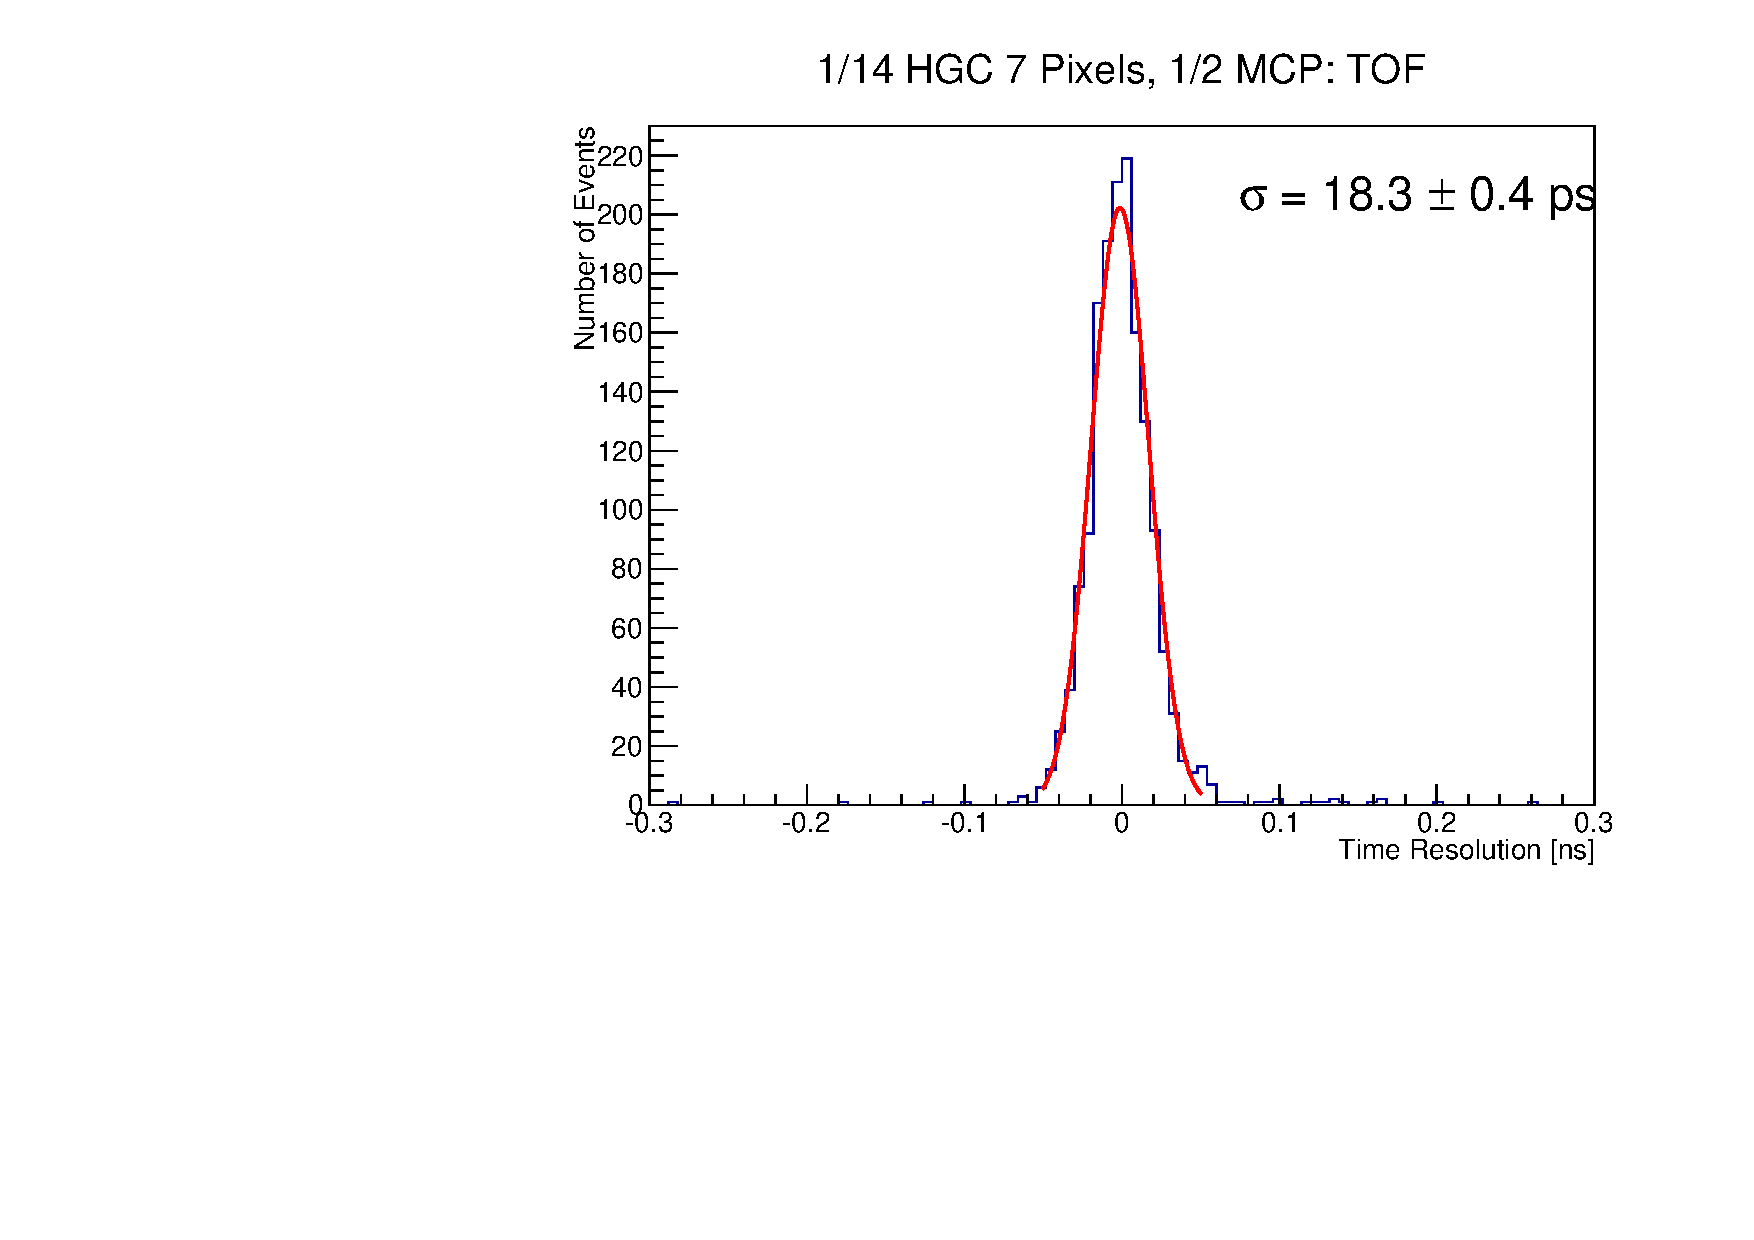
\includegraphics[width=.49\textwidth]{deltaT_PicoSilEqual_MCP_Equal104.pdf}
	\caption{Implementation of basic methods 1 (left) and 2 (right) as described in the text. }
	\label{fig:m12}
\end{figure}

Smarter ways to combine the HGC layer with the Photonis MCP includes weighting each pixel and the Photonis by their event or total charge. 
Mathematically, these methods would be given by,

\[
\Delta t_i = 
\dfrac{ \Delta t_{MCP_i} q_{MCP_i} +
	\sum\limits_{all\ pixels} \Delta t_{HGC_i} q_{HGC_i} }
	{ q_{MCP_i} +
	\sum\limits_{all\ pixels} q_{HGC_i} }
\]

\[
\Delta t_i = 
\dfrac{ \Delta t_{MCP_i} Q_{MCP} +
	\sum\limits_{all\ pixels} \Delta t_{HGC_i} Q_{HGC} }
	{ Q_{MCP} +
	\sum\limits_{all\ pixels} Q_{HGC} }
\]

Figure \ref{fig:HGC_MCP_event_total_104} gives the TOF histograms using these combination methods. While the total charge method time resolution shows an undeniable improvement, the event charge method time resolution of 14.2 ps is better than any HGC layer combination (Figure \ref{fig:HGC_event_total_MPV_104}) but worse than the resolution of just the Photonis (Figure \ref{fig:center_MCP_104}).

\begin{figure}[h]
\centering
\begin{minipage}[t]{.64\textwidth}
	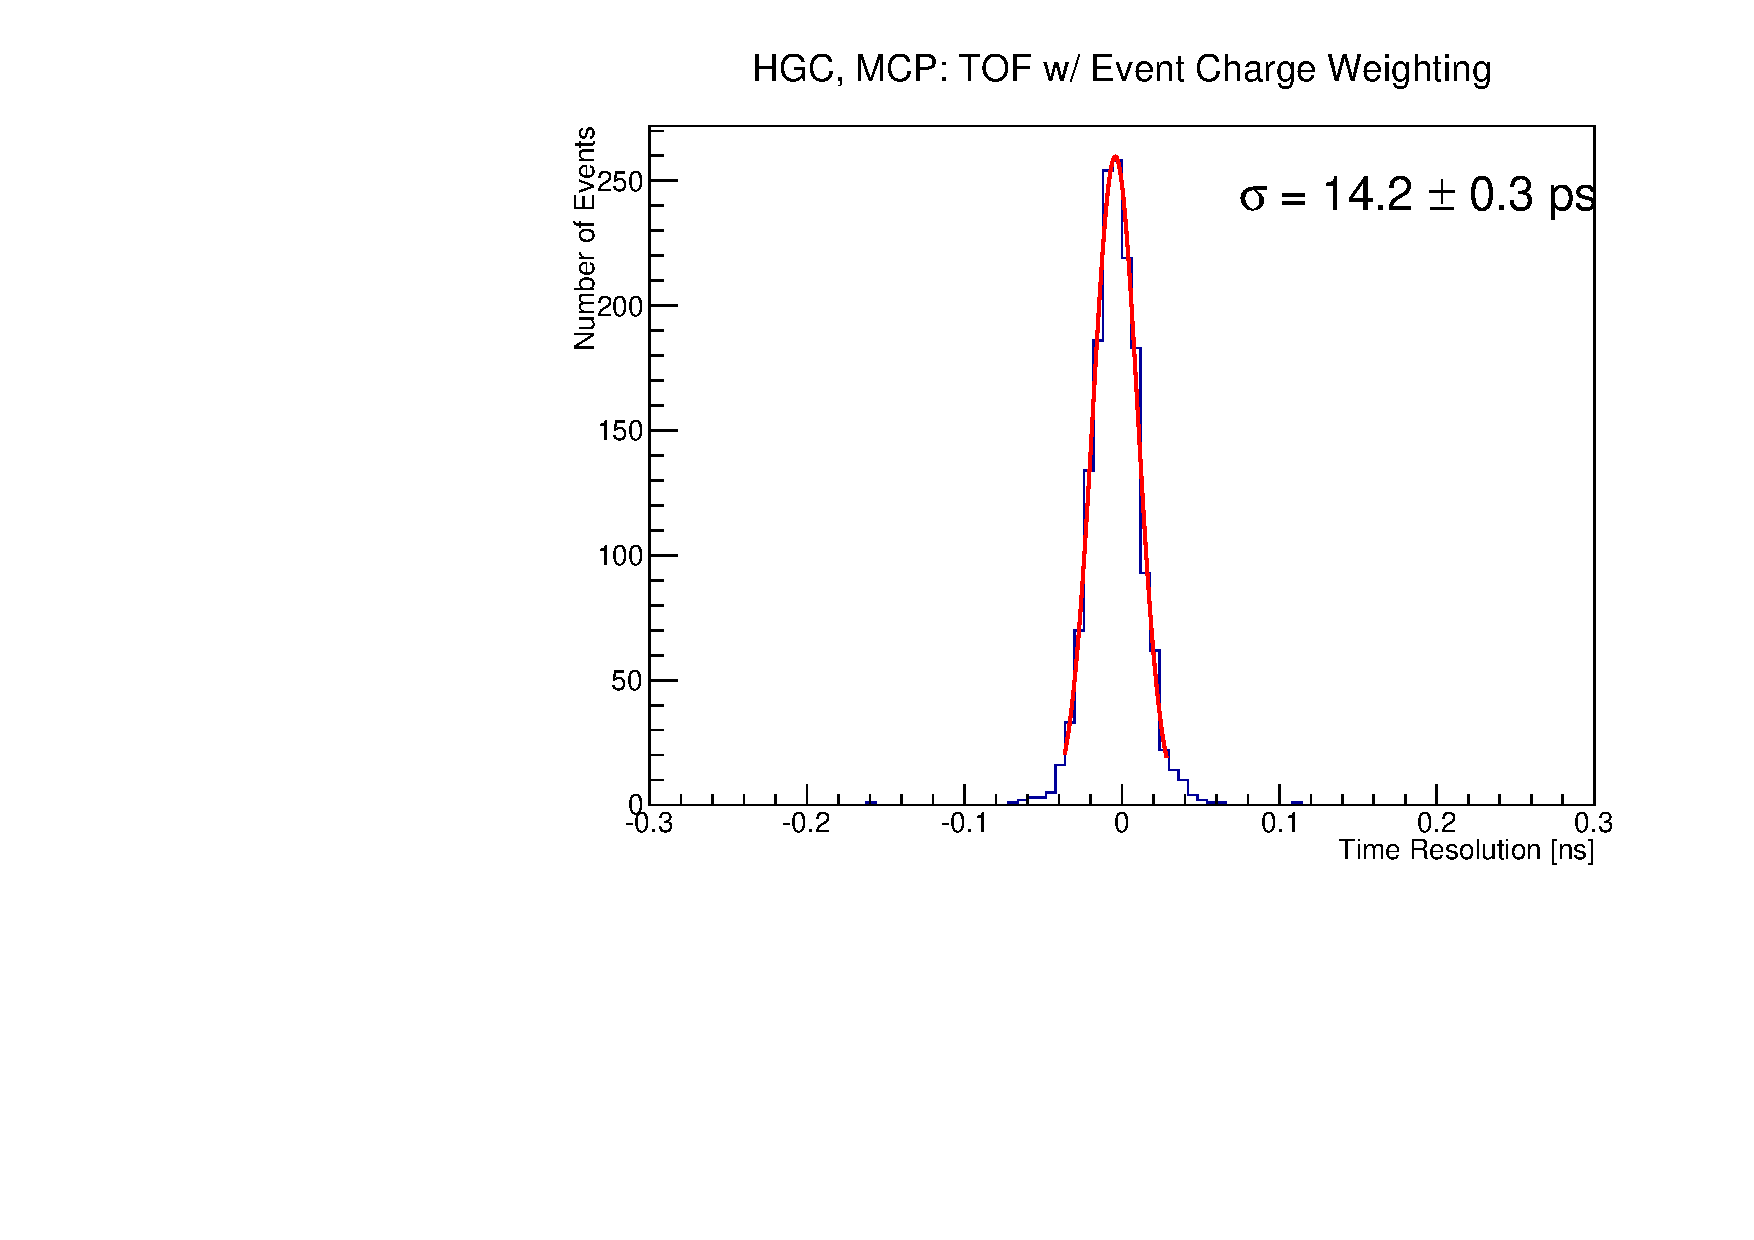
\includegraphics[width=.49\textwidth]{deltaT_PicoSil_MCP_EventCharge104.pdf}
	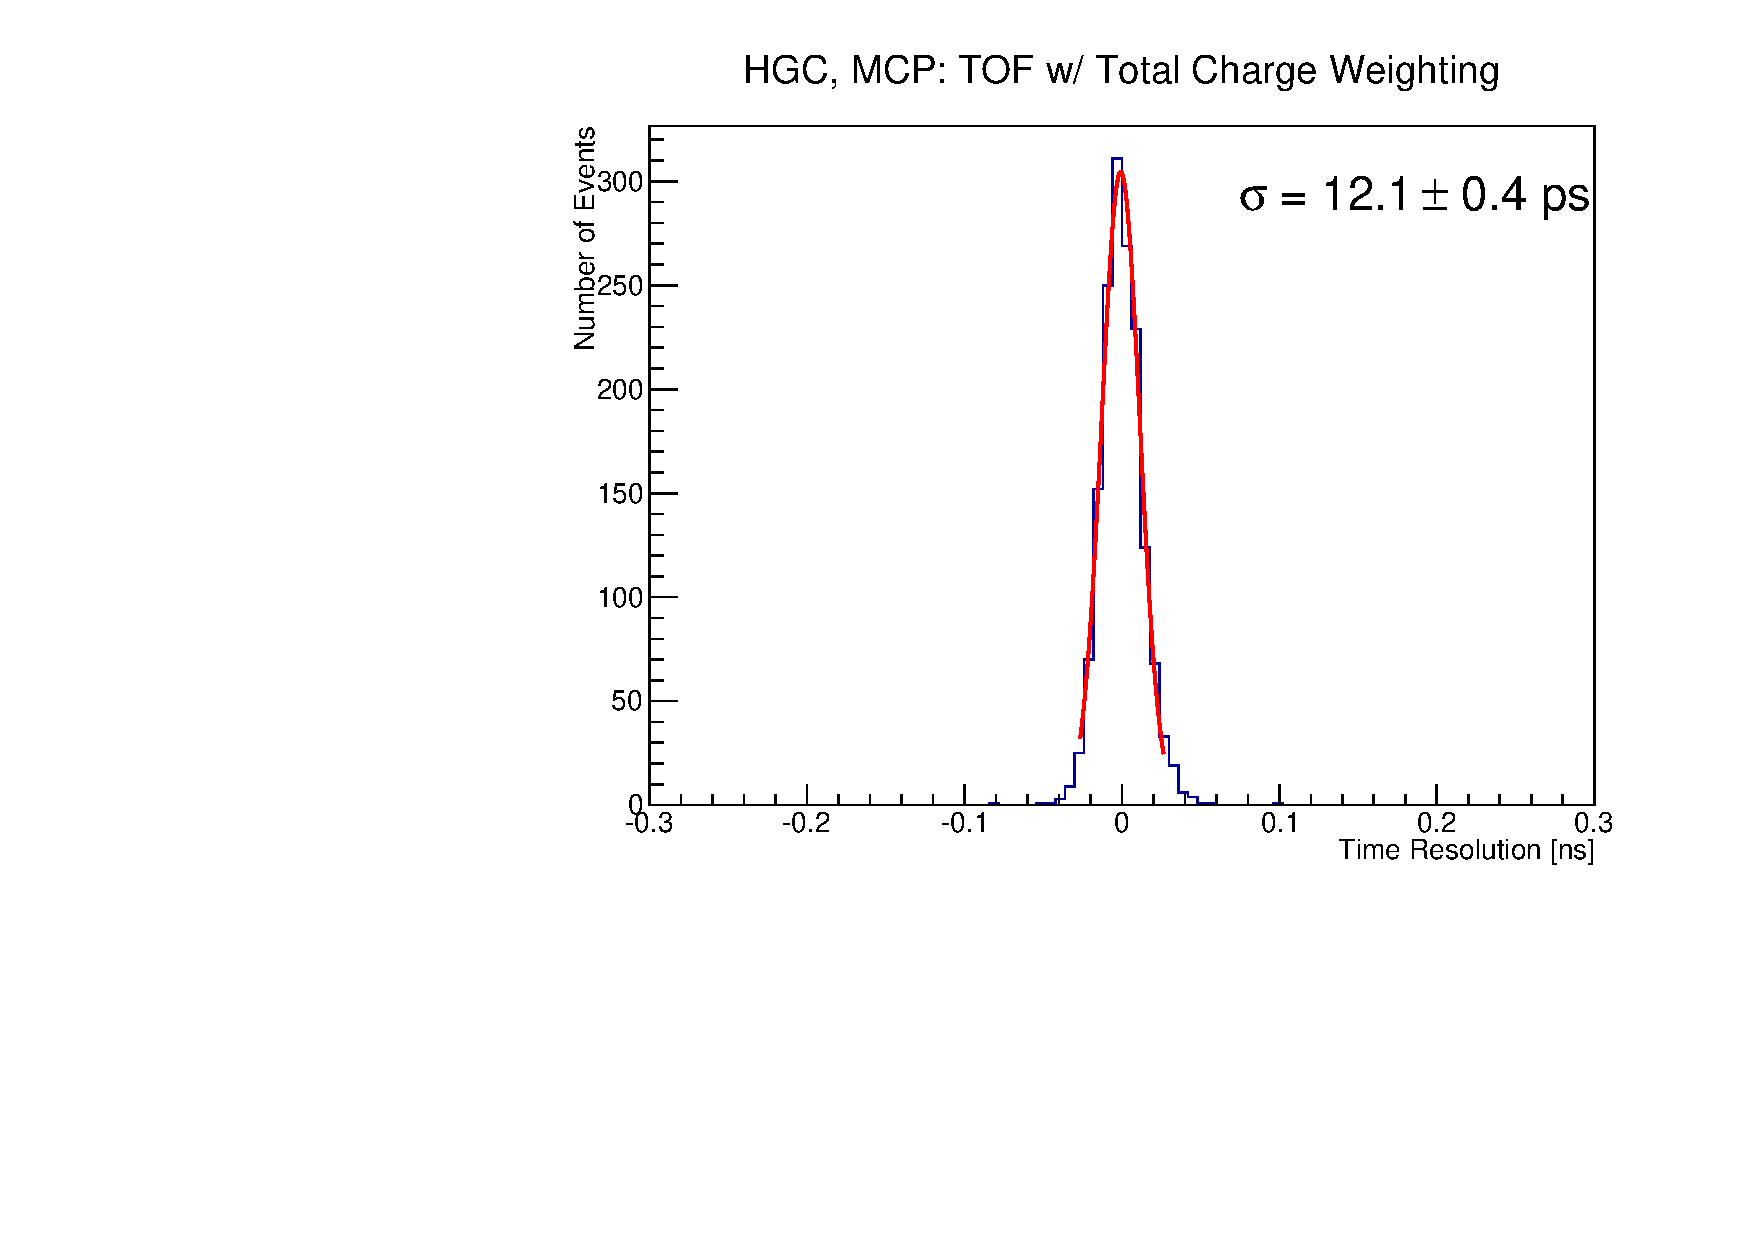
\includegraphics[width=.5\textwidth]{deltaT_PicoSil_MCP_TotalCharge104.pdf}
	\caption{TOF histograms of the HGC pixels and Photonis MCP, using event (left) and total (right) charge weighting. }
	\label{fig:HGC_MCP_event_total_104}
\end{minipage} \hfill
\begin{minipage}[t]{.32\textwidth}
	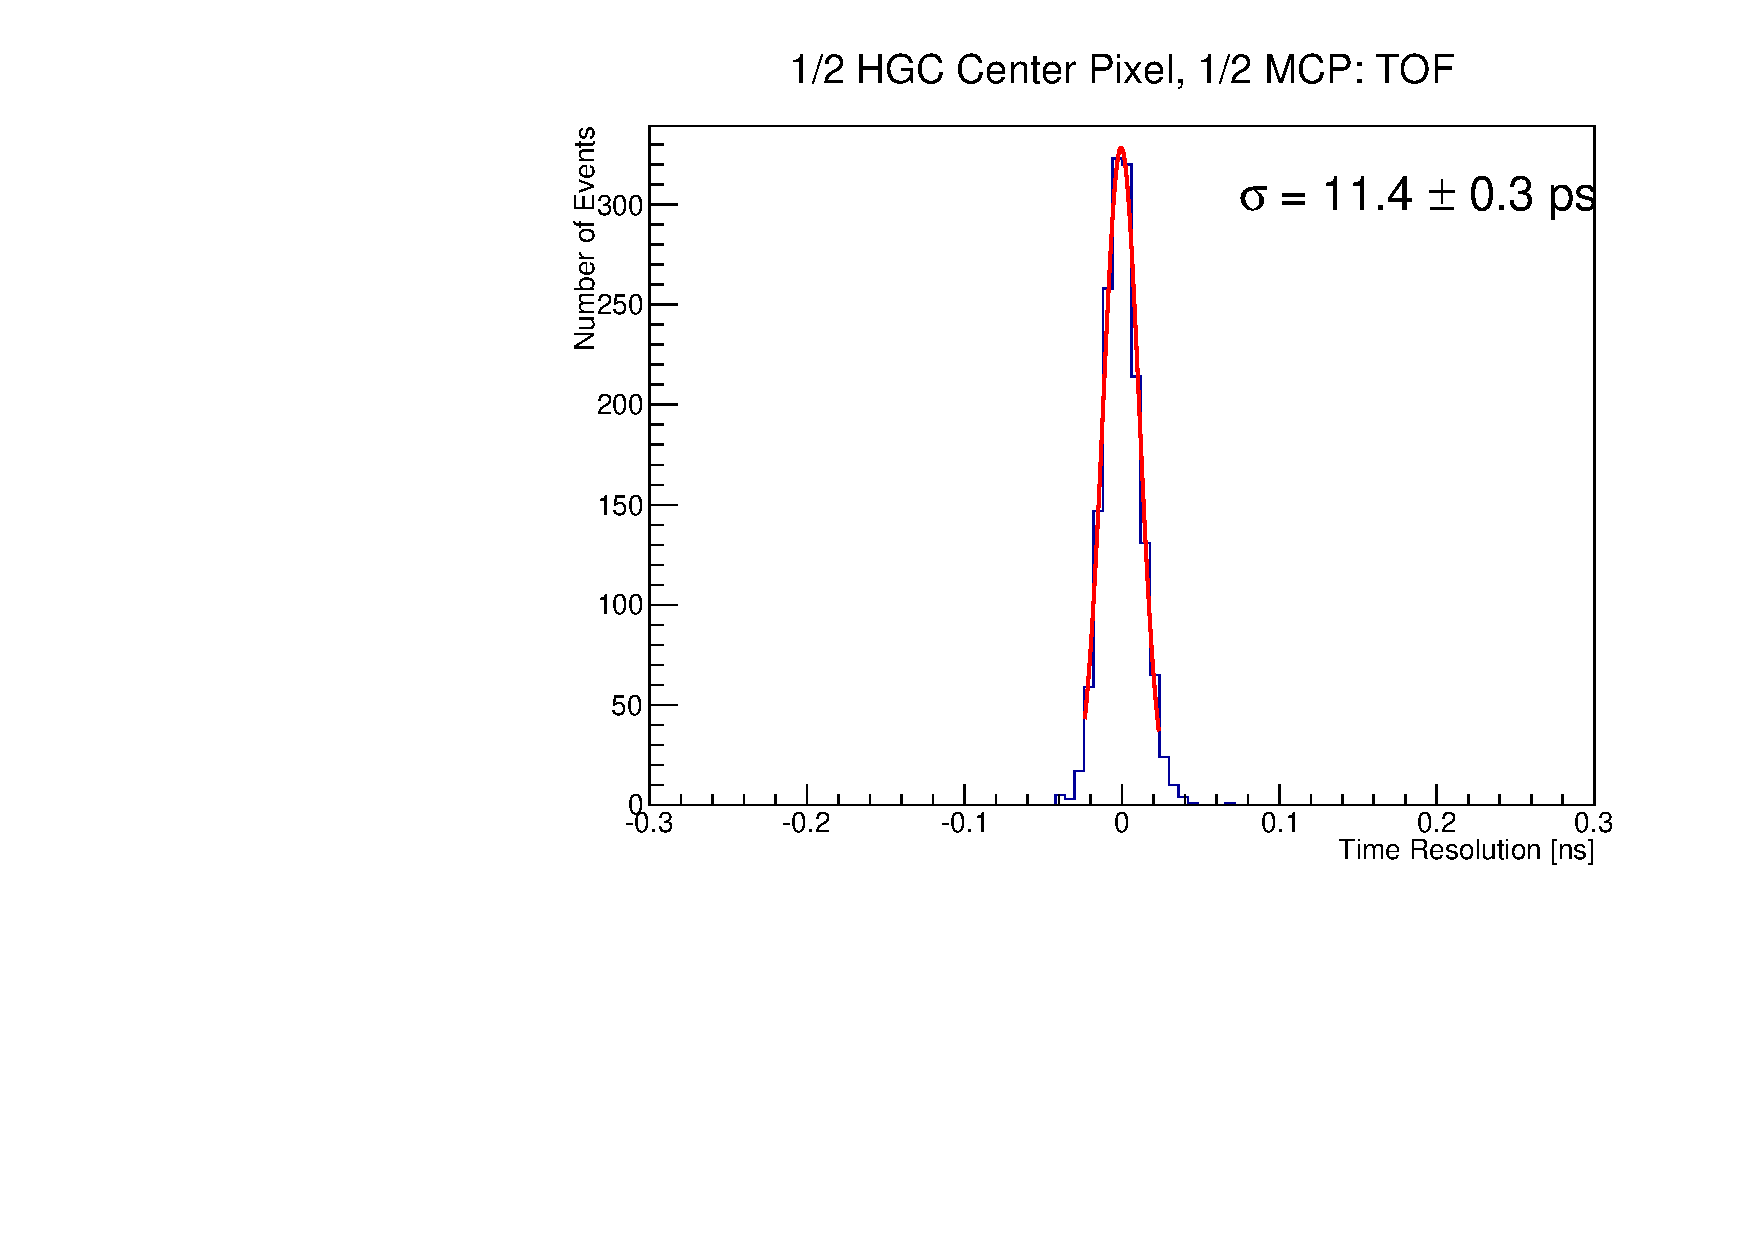
\includegraphics[width=\textwidth]{deltaT_Center_MCP_Equal104.pdf}
	\caption{TOF histogram weighting $\Delta t_{Center}$ and $\Delta t_{Photonis}$ by $\frac{1}{2}$.}
	\label{fig:CenterMCPEqual104}
\end{minipage}
\end{figure}

It turns out, however, that an HGC/Photonis combination using just charges is not the most accurate way to weight each detector. 
The first indication that there may be a smarter method comes from the equal weighting combination of the HGC center pixel (left Figure \ref{fig:center_MCP_104}; 15.9 ps) and the Photonis. 
Figure \ref{fig:CenterMCPEqual104} shows this combination. 
While the total charge-combined HGC layer has a better time resolution than the center pixel, the latter's equal combination with the Photonis is significantly better (11.4 ps compared to 12.1 ps). 
The equal weighting between devices is better than one of the charge weightings because it approximates that the same amount of charge flows into both detectors.
Even though the charge is not actually equal, this approximation is better than using the charge weighting \textit{because the relative gain of the HGC and Photonis is not known}. 
Put another way, a particle of a specific energy detected in the HGC would not return the same charge as a detection in the Photonis. 
Therefore, a better way to weight the $\Delta t$ values would be to do either an event charge, total charge, or charge MPV weighting for the HGC pixel $\Delta t$'s, then weight that value equally with the Photonis $\Delta t$ (Figure \ref{fig:HGCMCP_event_total_MPV_104}). 
While the event charge weighting again gives the worst time resolution, the other two methods have a time resolution that is essentially the same as the HGC center pixel equally weighted with the Photonis MCP. 

\begin{figure}[h]
	\centering
	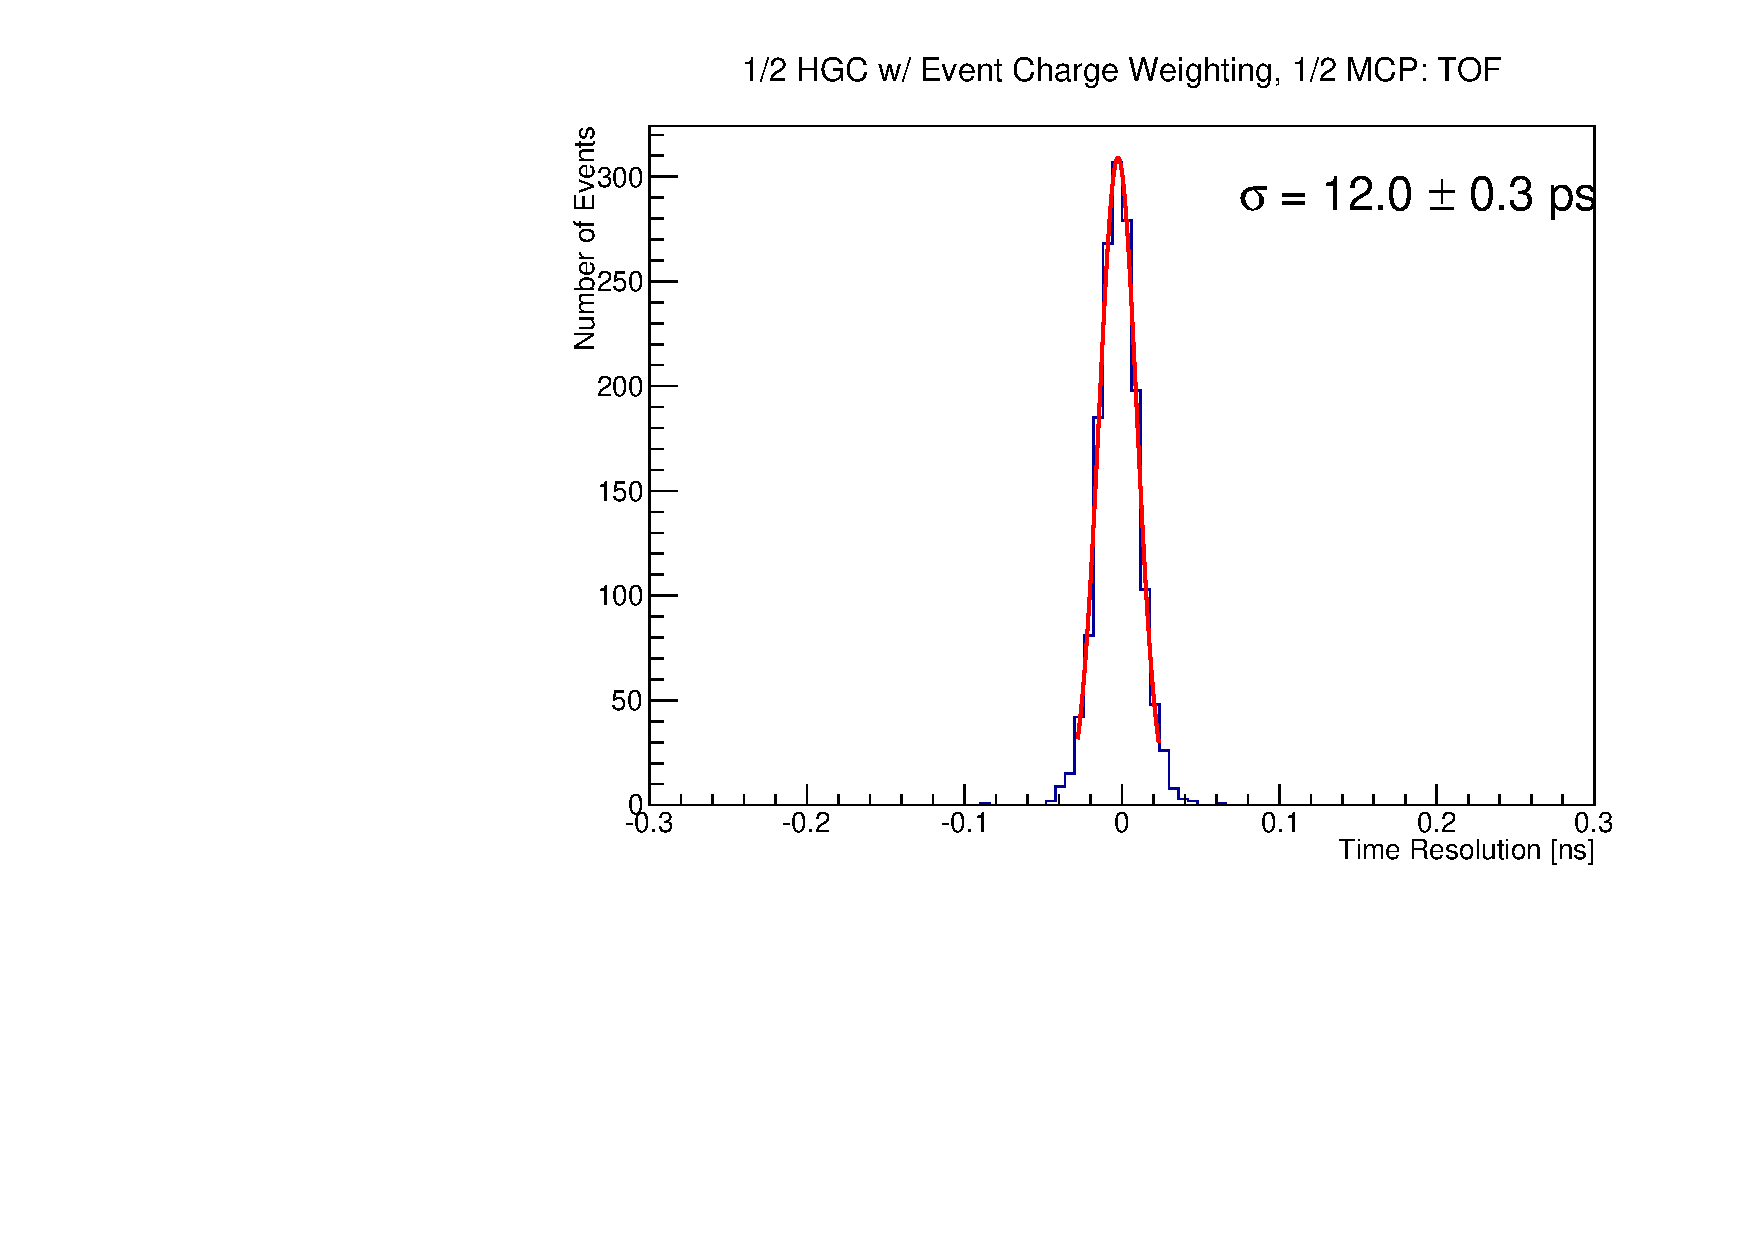
\includegraphics[width=.32\textwidth]{deltaT_PicoSilEventCharge_MCP_Equal104.pdf}
	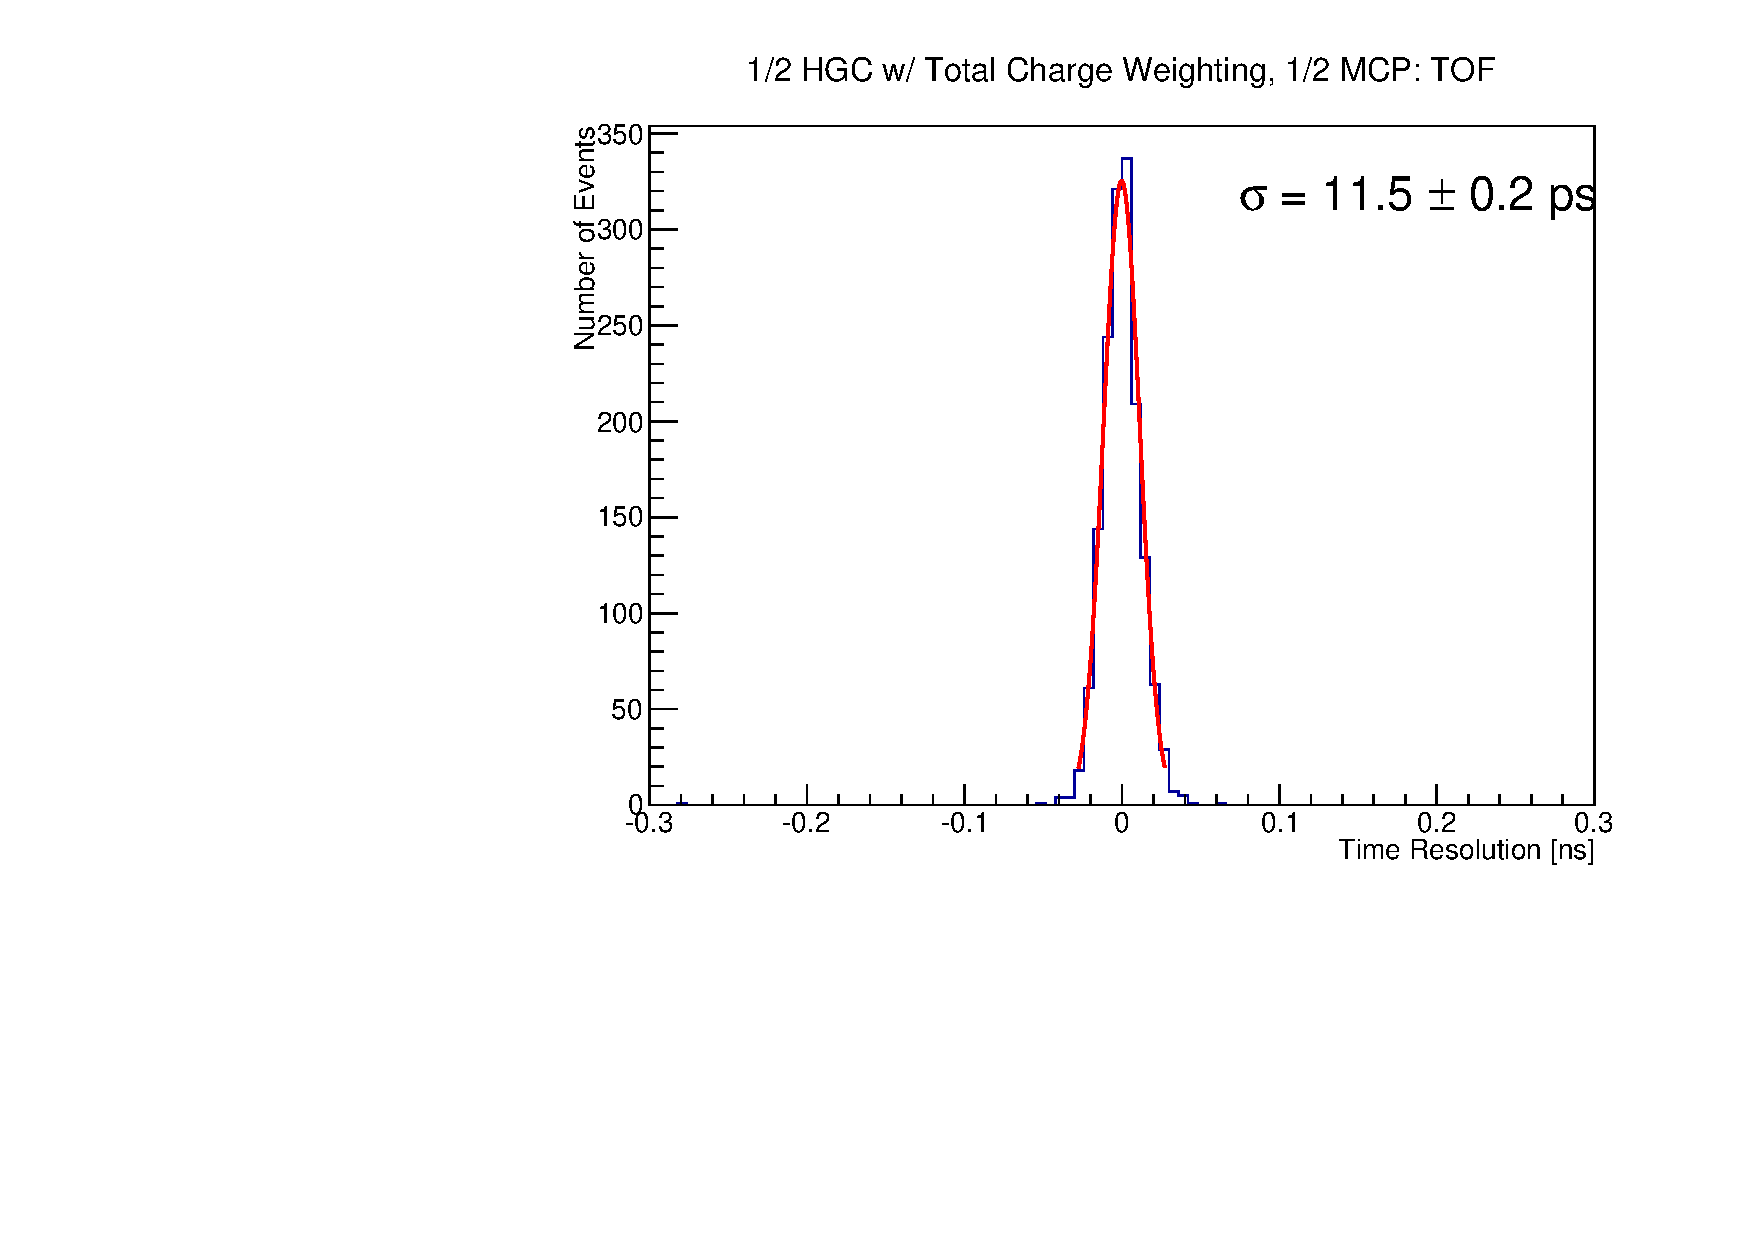
\includegraphics[width=.32\textwidth]{deltaT_PicoSilTotalCharge_MCP_Equal104.pdf}
	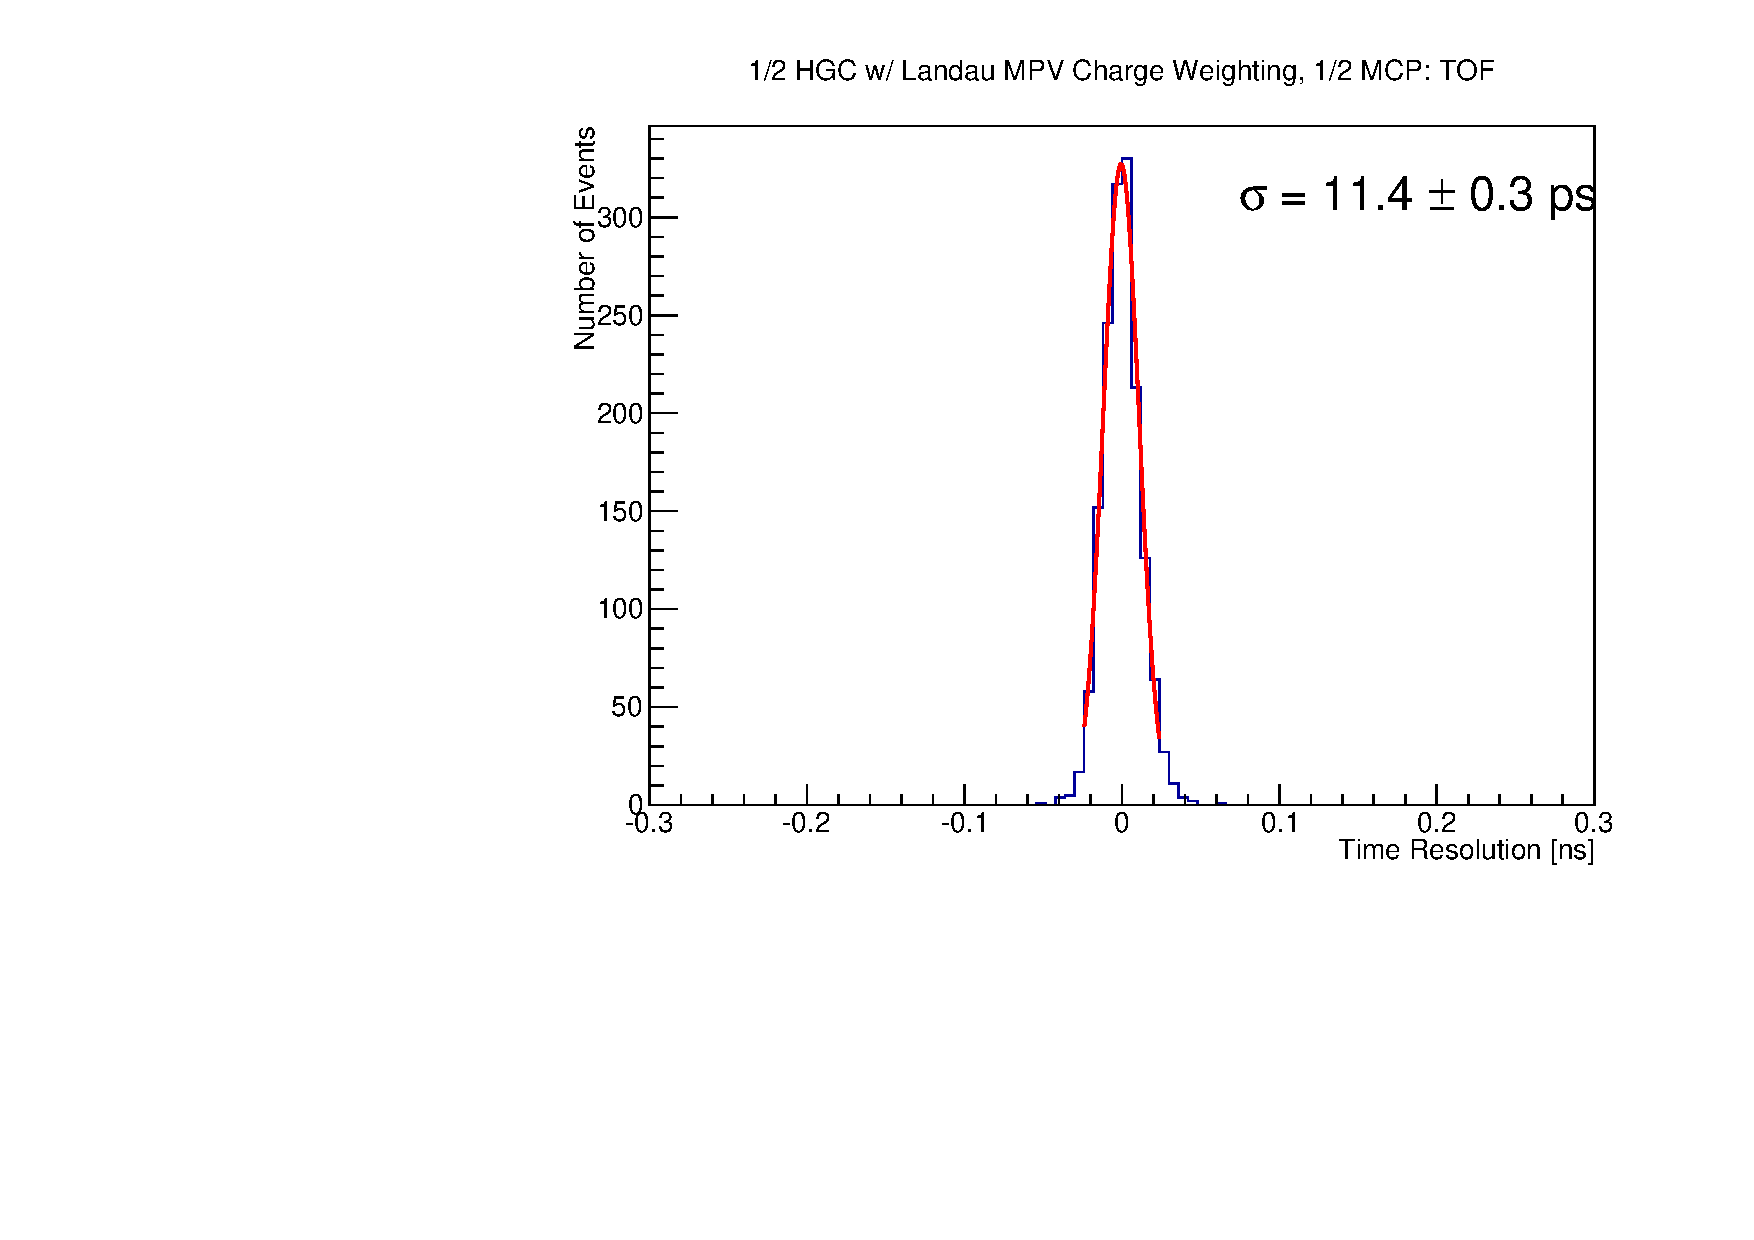
\includegraphics[width=.32\textwidth]{deltaT_PicoSilLandauCharge_MCP_Equal104.pdf}
	\caption{TOF histogram weighting $\Delta t_{HGC}$ and $\Delta t_{Photonis}$ by $\frac{1}{2}$, with $\Delta t_{HGC}$ computed via event (left), total (middle), and MPV (right) charge weightings.}
	\label{fig:HGCMCP_event_total_MPV_104}
\end{figure}

This lack of improvement is most likely due to the relatively great time resolution of the central pixel compared to the inner ring pixels, which have a $\sigma$ that is around 4 times larger. 
Adding in the 6 ring pixels the time resolution only improved from $15.9 \pm 0.4$ ps to $15.5 \pm 0.4$ ps.
This improvement is small because the worse time resolutions of the outside pixels cannot contribute much to the already-good center pixel.
In this experiment, the test beam was focused onto the center pixel, which improved its time resolution compared to the other pixels. 
At the LHC, one pixel will not always be favored over the others in bunch crossings, and the most energetic part of the interaction may not interact with one of the pixels, so the pixel resolutions are expected to be similar.
While it does not seem useful in this experiment to add in the ring pixels, perhaps if they had a similar time resolution, adding them would lead to bigger improvements.
This statement is tested below.

Note that the time resolution values and their relative sizes given in the plots above are for this specific configuration.
Analyzing other runs will lead to changes in these values. 
The absorber thickness, distance, and type, and the beam energy contribute to the varying values of $\sigma$.

\section{SKIROC2 Emulation}
For calorimetry at CMS, the SKIROC2 ASIC reads out the pulse data from the detectors.
Sacrificing accuracy for speed, the SKIROC2 chip has a digital jitter affecting the pulse time values, which places a lower bound on $\sigma$. 

\subsection{Background}
This jitter has previously been observed to model a Gaussian distribution of $\sigma=50$ ps, centered around 0.
Thus, if a detector consistently measured pulses at time $X$, then plotting all of these time values would be essentially a Dirac Delta function.
If these values were then read out by the SKIROC2 chip, then for enough events, plotting these new values would give a Gaussian of $\sigma = 50$ ps, $\mu = X$.
However, as explained above, the initial time values are already Gaussian distributed, so reading the data out would return a convolution of the two distributions. 
In other words, the new distribution will be a Gaussian of $\sigma > 50$ ps.

In order to simulate how multiple HGC layers with multiple pixels at CMS can improve the time resolution, each pixel's pulse time can be \textit{smeared} by 50 ps, according to a random sampling from a Gaussian distribution.
This new smeared time can then be used to calculate the $\Delta t$ value by subtracting it from the Photek's pulse time, which is not smeared.

From Figure \ref{fig:mathematica_plot}, it can be observed that pixels with different initial $\sigma$ values will approach the same value when smeared by large amounts. 
This smearing can be used to test whether combining detectors of similar time resolution will be able to significantly improve the overall time resolution.

\begin{figure}[h]
	\centering
	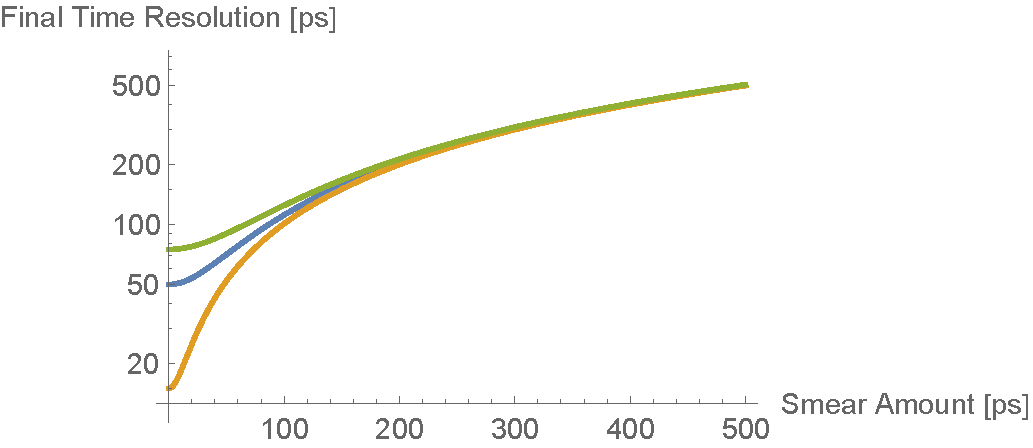
\includegraphics[width=.75\textwidth]{mathematica_plot.pdf}
	\caption{After being smeared by a large amount, detectors with different time resolutions (15 ps, 50 ps, 75 ps) approach the same value. Plotted in Wolfram Mathematica.}
	\label{fig:mathematica_plot}
\end{figure}

\subsection{50 ps Smear}
\subsubsection{Add Pixels Individually: All Pixels}
After smearing each pixel in the HGC by 50 ps, there are many ways to combine the $\Delta t$ values. 
Before smearing, any form of equal weighting led to worse time resolutions, because the center pixel should have been weighted more.
However, as seen in Figure \ref{fig:mathematica_plot}, a 50 ps smear makes the time resolutions of the detectors closer. 
Yet, the inner ring pixels initially had time resolutions near 70-80 ps, so they still may not help as much as if they were the same.

In this case, it may still be useful to combine with some form of charge weighting, since the center pixel most likely should be weighted relatively heavily.
This way, the lower time resolution of the center pixel is emphasized.
However, equal weighting becomes a more valid method for larger smears, since the correlation between charge and a small $\sigma$ disappears.

Furthermore, it is interesting to observe how the time resolution will improve with the addition of each pixel. 
This analysis can help determine how many pixels can be added before the time resolution stops improving.
Because only a handful of event cuts are passed by all 6 inner ring HGC pixels and the center pixel, adding pixels should not be able to reduce the events.
In order to maintain a high event number, when two pixels X and Y are added together, the union of the events they pass -- instead of the intersection -- shall be the new number of events.
The intersection of passed events shall be the combined $\Delta t$'s, and the remaining events shall simply use the individual $\Delta t$.

Each additional pixel shall be combined in decreasing order of number of events passed, since those detectors have the larger chance of improving the time resolution.
Figure \ref{} shows the addition of each smeared pixel using an equal weighting method. 
Figure \ref{} shows the smeared pixel addition using the charge MPV weighting method, since it appeared to be the best method/equally as good as the total charge method.

%%% INCLUDE FIGURE WITH 7 PLOTS HERE %%% 3 rows: 2-3-2

%%% INCLUDE FIGURE WITH 7 PLOTS HERE %%%

\subsubsection{Add Pixels Individually: Exclude Center Pixel}
The improvement in the previous section is not good enough to reach the pre-smearing time resolutions. 
Perhaps combining the inner ring pixels without incorporating the center pixel will show a bigger improvement ($\sigma_0-\sigma_f$), due to combining detectors of similar time resolution. 
Figure \ref{} shows the addition of each smeared pixel using an equal weighting method.

%%% INCLUDE FIGURE WITH 6 PLOTS HERE %%%

\subsection{500 ps Smear}
\subsubsection{Add Pixels Individually: All Pixels}
In order to illustrate the strength of the equal weighting method over charge-based methods at high smear values, a 500 ps Gaussian smearing is applied to each pixel.
Here the charge should have no correlation to the time resolution of each detector.
Additionally, the center pixel should have the same weighting factor as any other pixel, since it has equally as bad of a resolution.

Figure \ref{fig:500psAll} shows the addition of each smeared pixel using an equal weighting method.

\begin{figure}[h]
\centering
	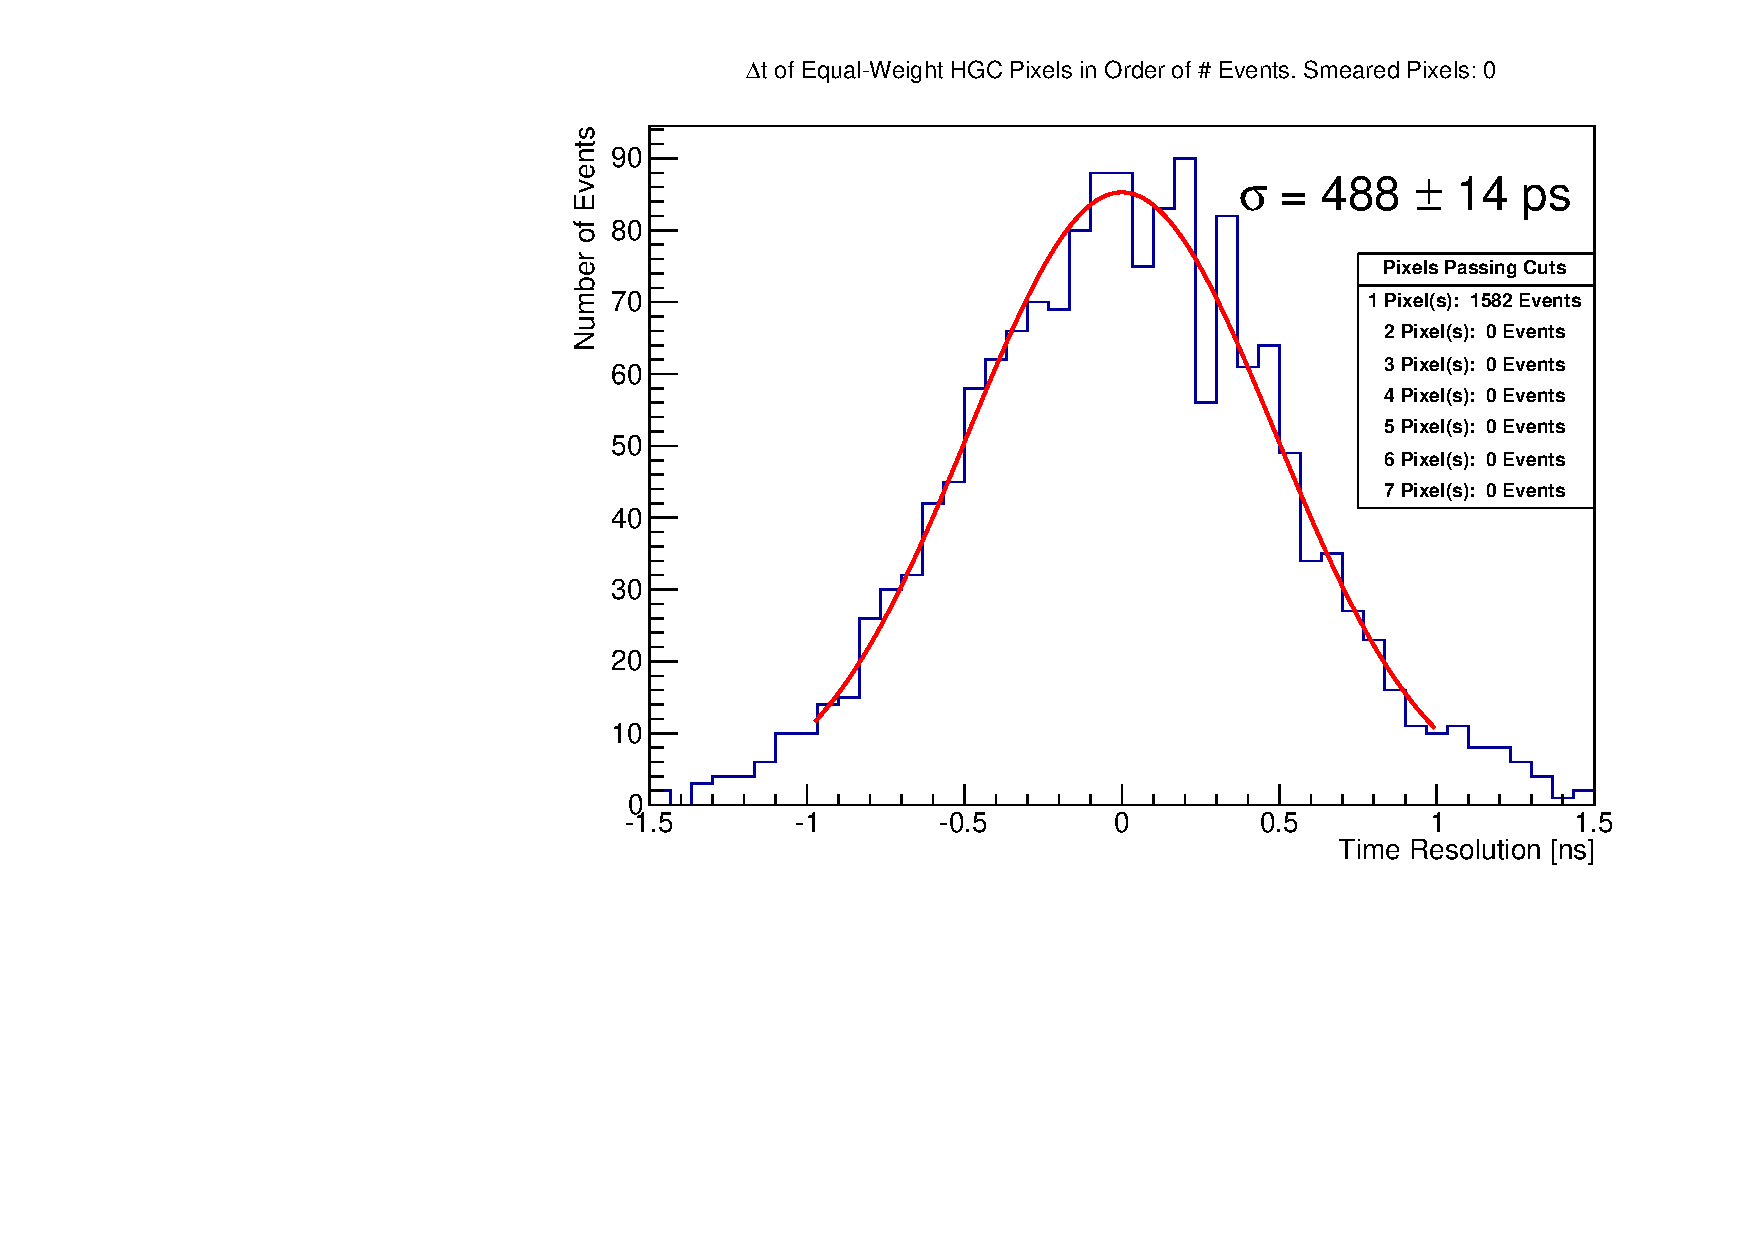
\includegraphics[width=0.4\textwidth]{SKIROC/SKIROC_1_Pixels.pdf}
	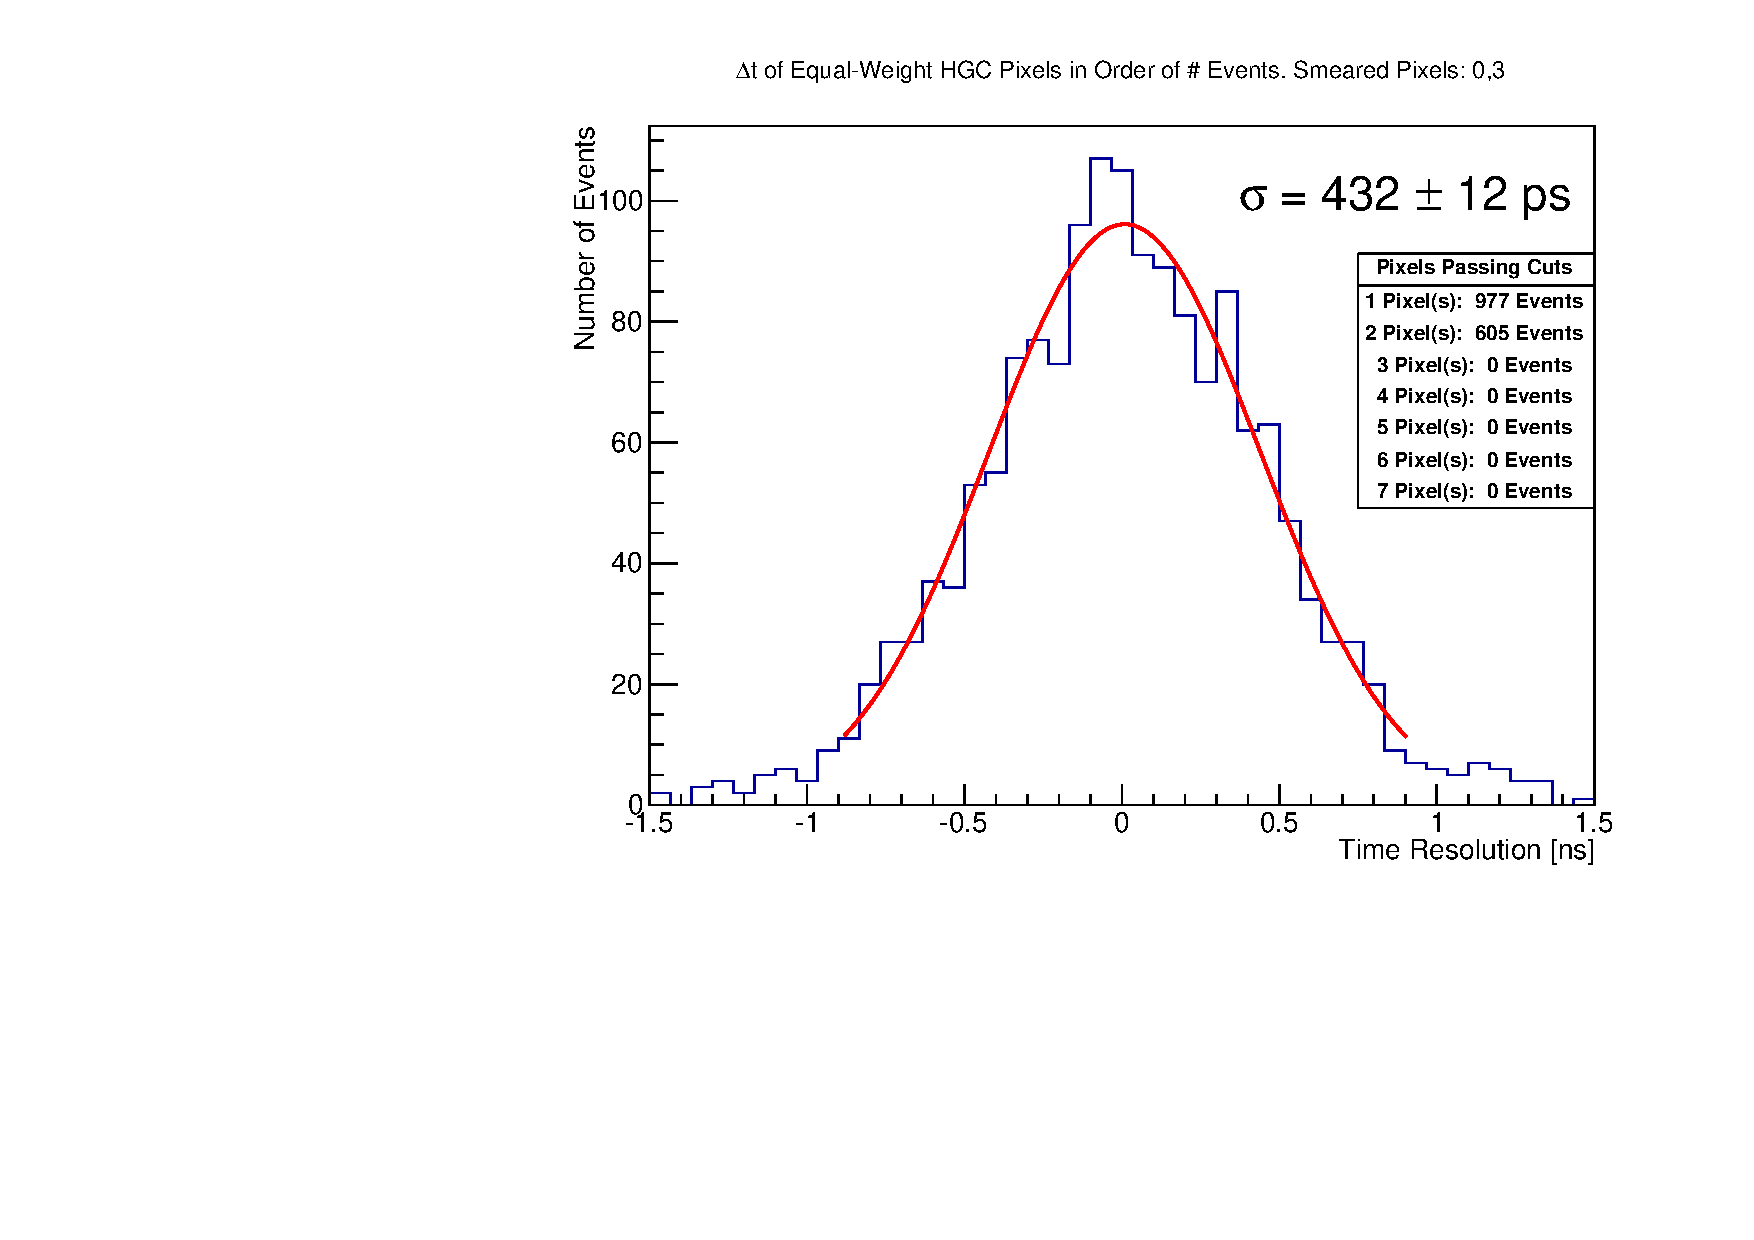
\includegraphics[width=0.4\textwidth]{SKIROC/SKIROC_2_Pixels.pdf}
	
	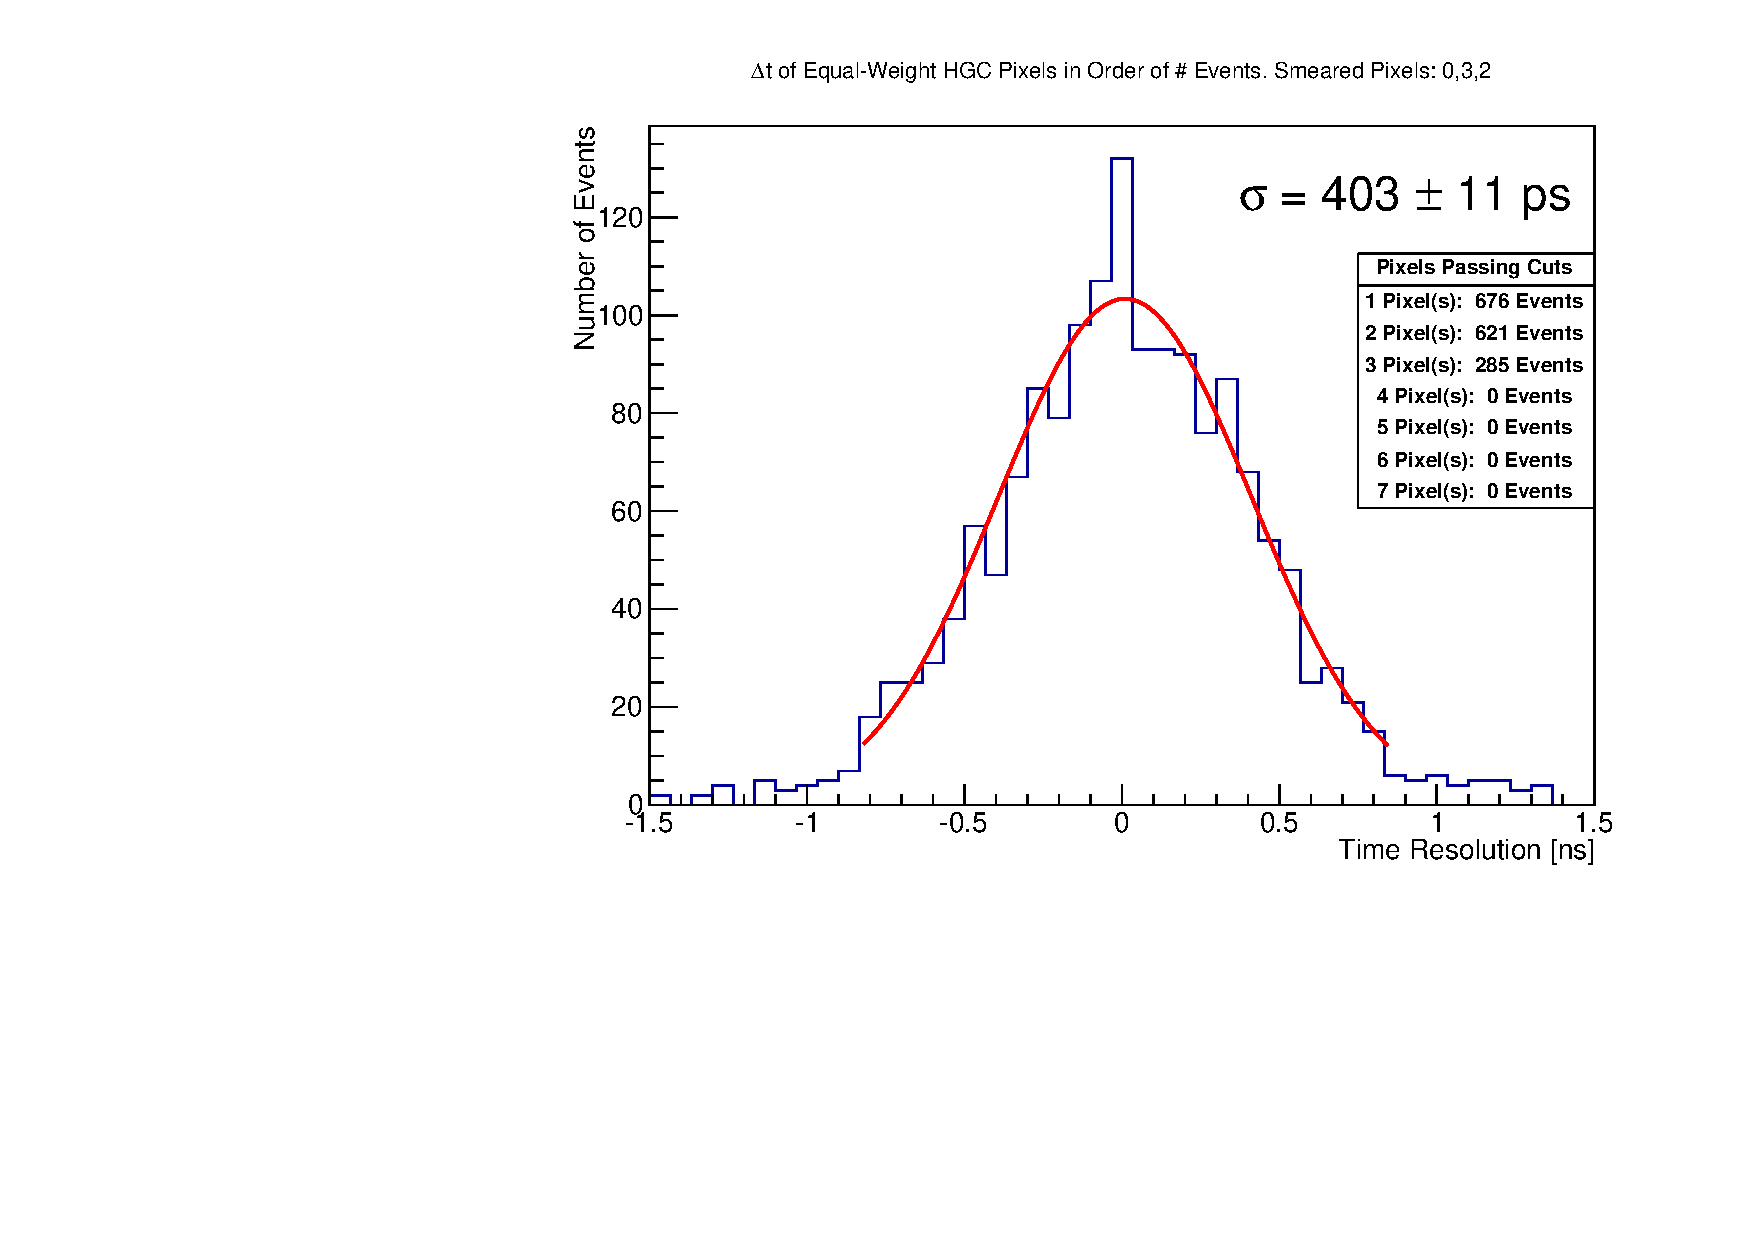
\includegraphics[width=0.32\textwidth]{SKIROC/SKIROC_3_Pixels.pdf}
	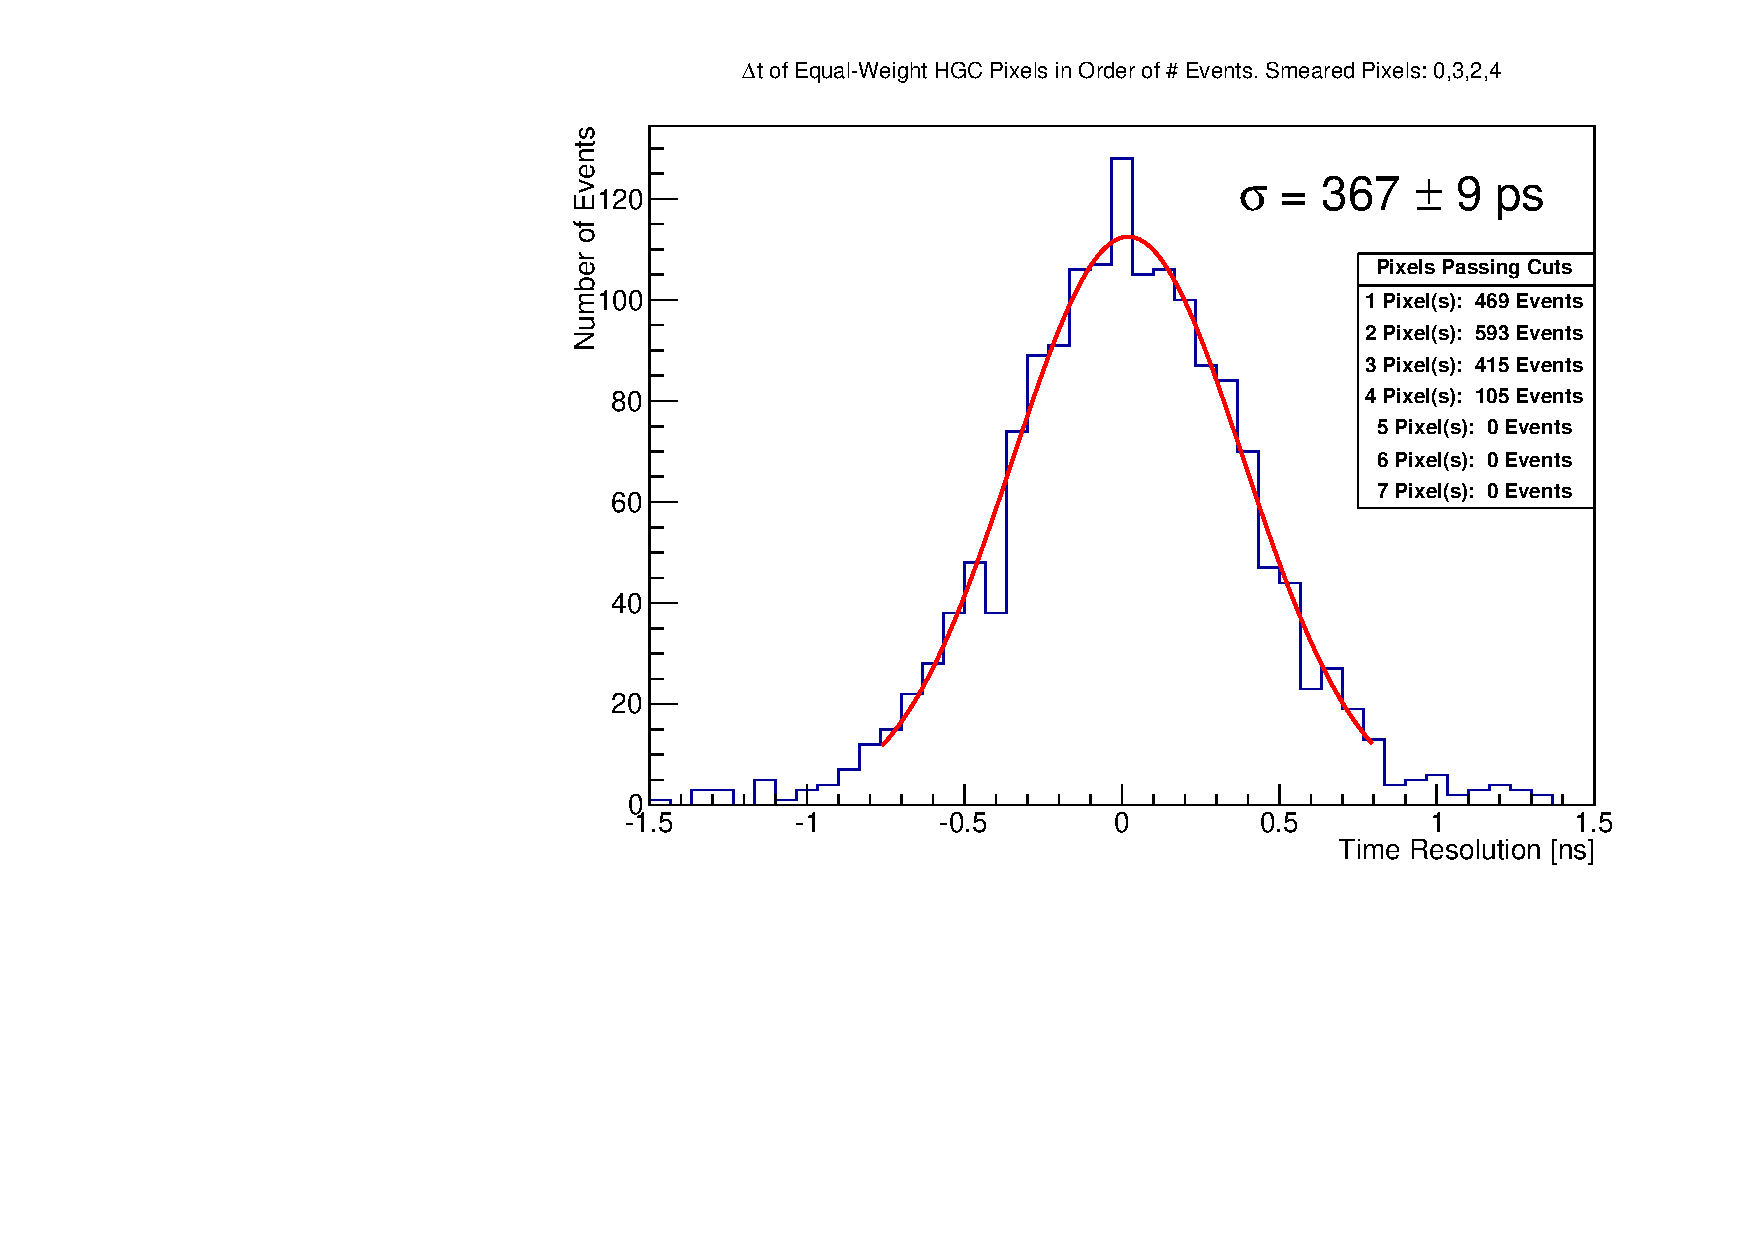
\includegraphics[width=0.32\textwidth]{SKIROC/SKIROC_4_Pixels.pdf}
	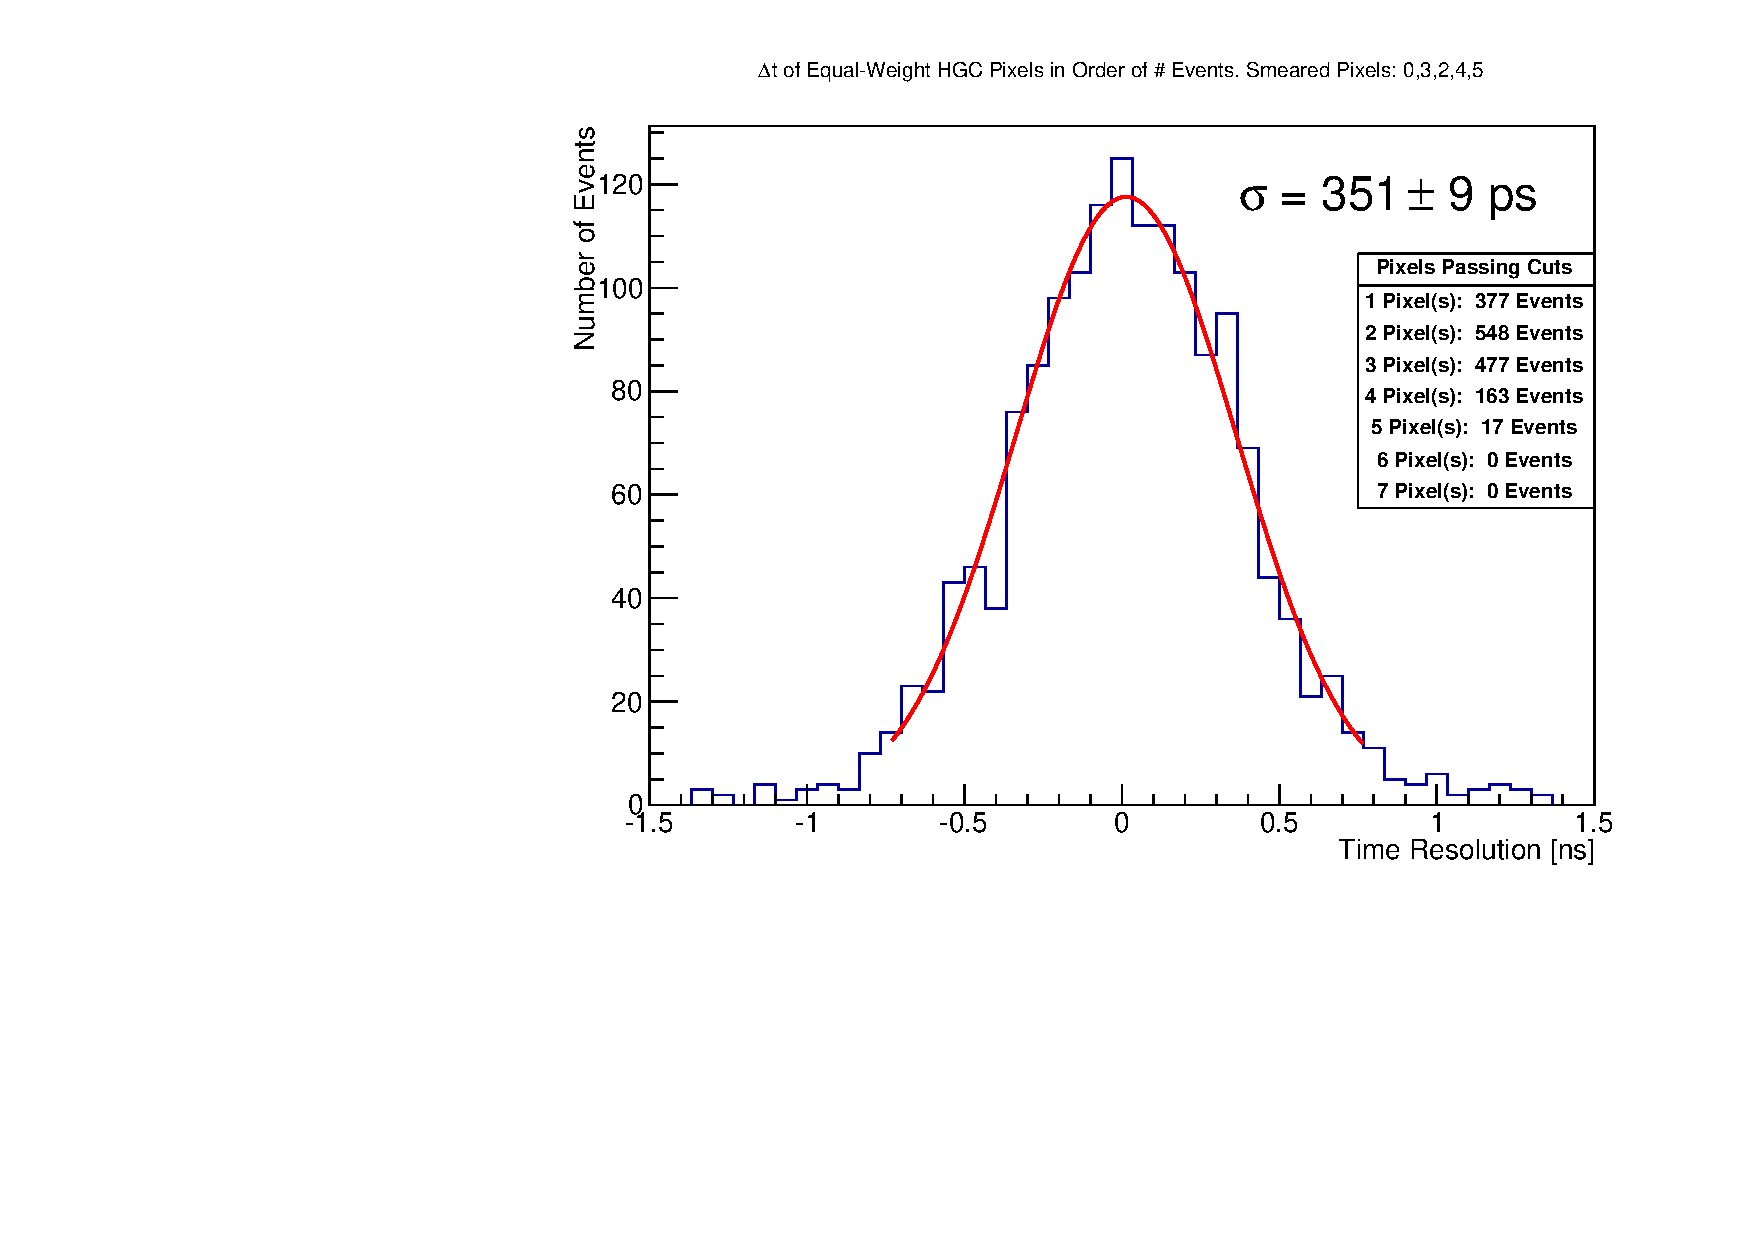
\includegraphics[width=0.32\textwidth]{SKIROC/SKIROC_5_Pixels.pdf}
	
	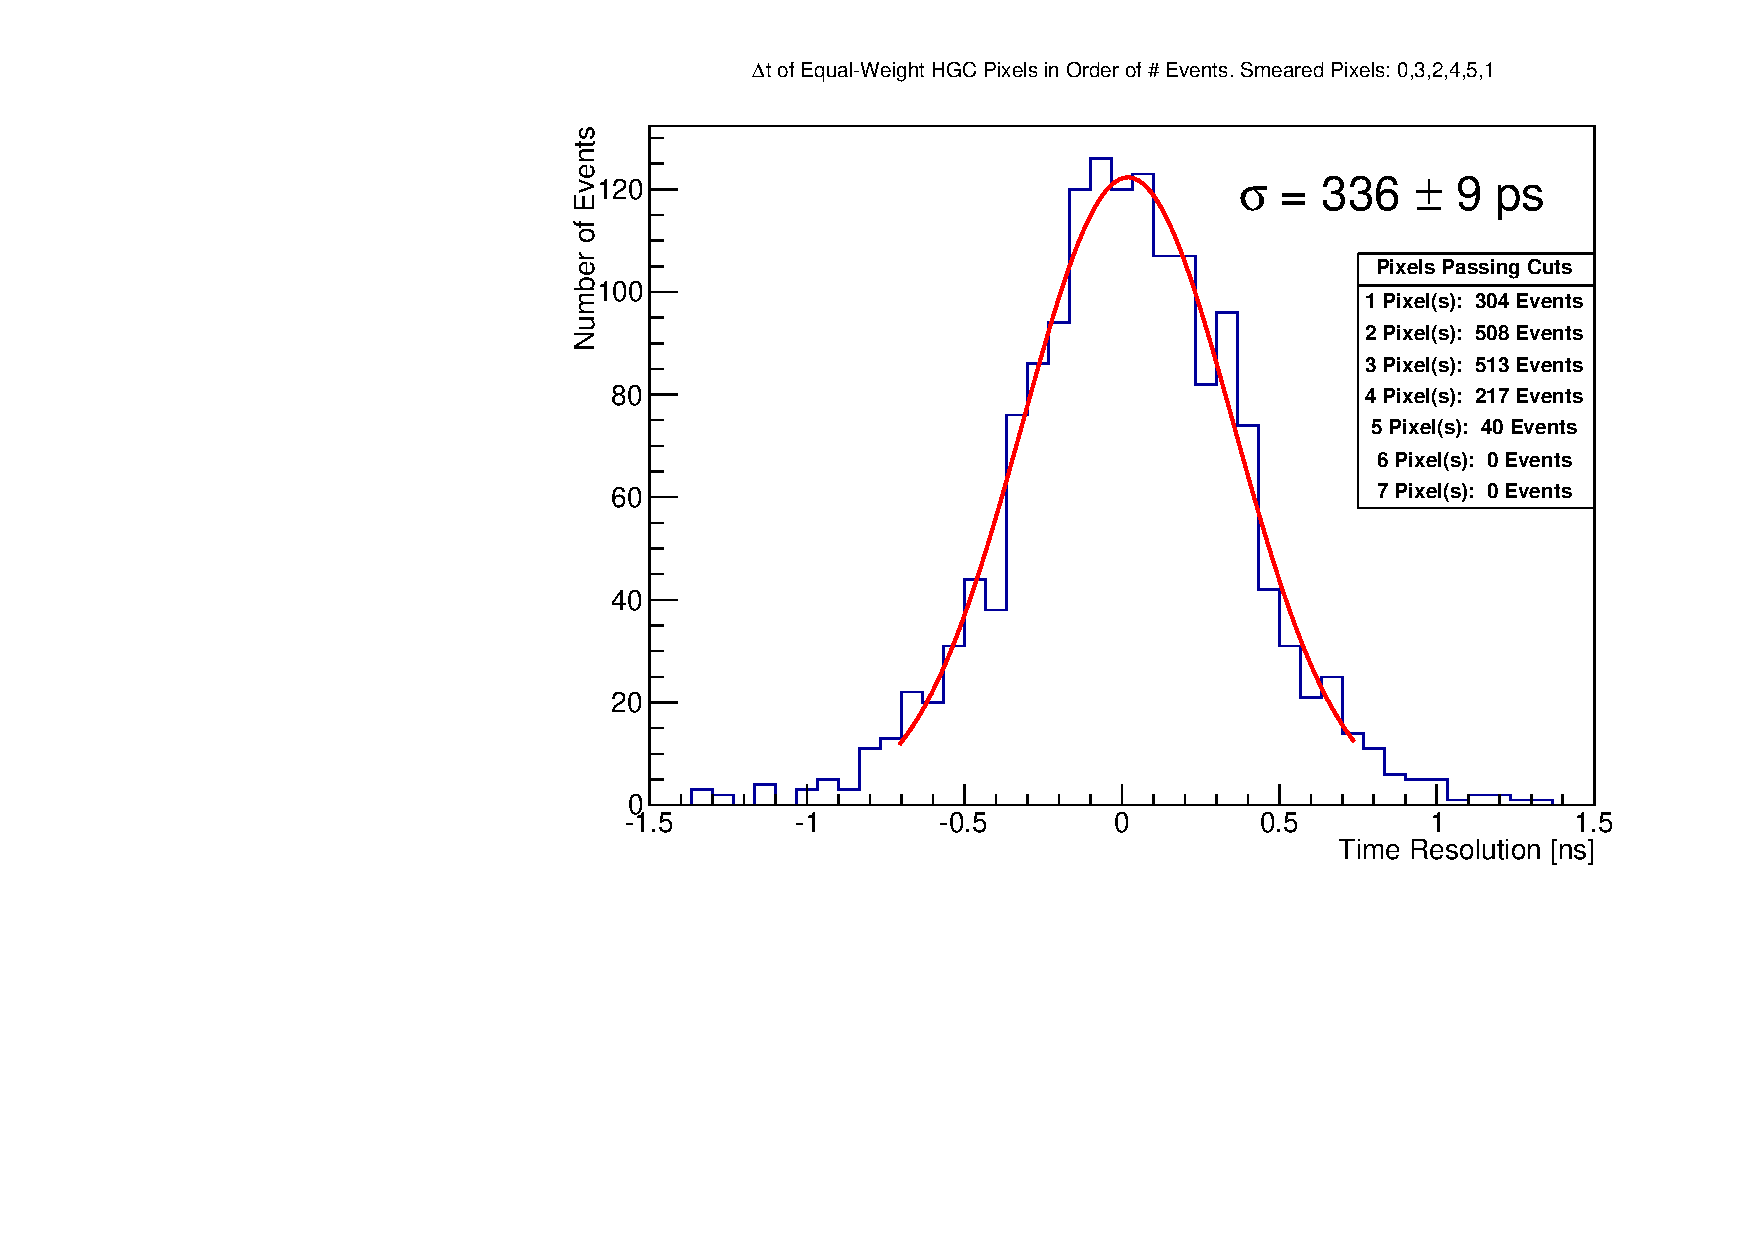
\includegraphics[width=0.4\textwidth]{SKIROC/SKIROC_6_Pixels.pdf}
	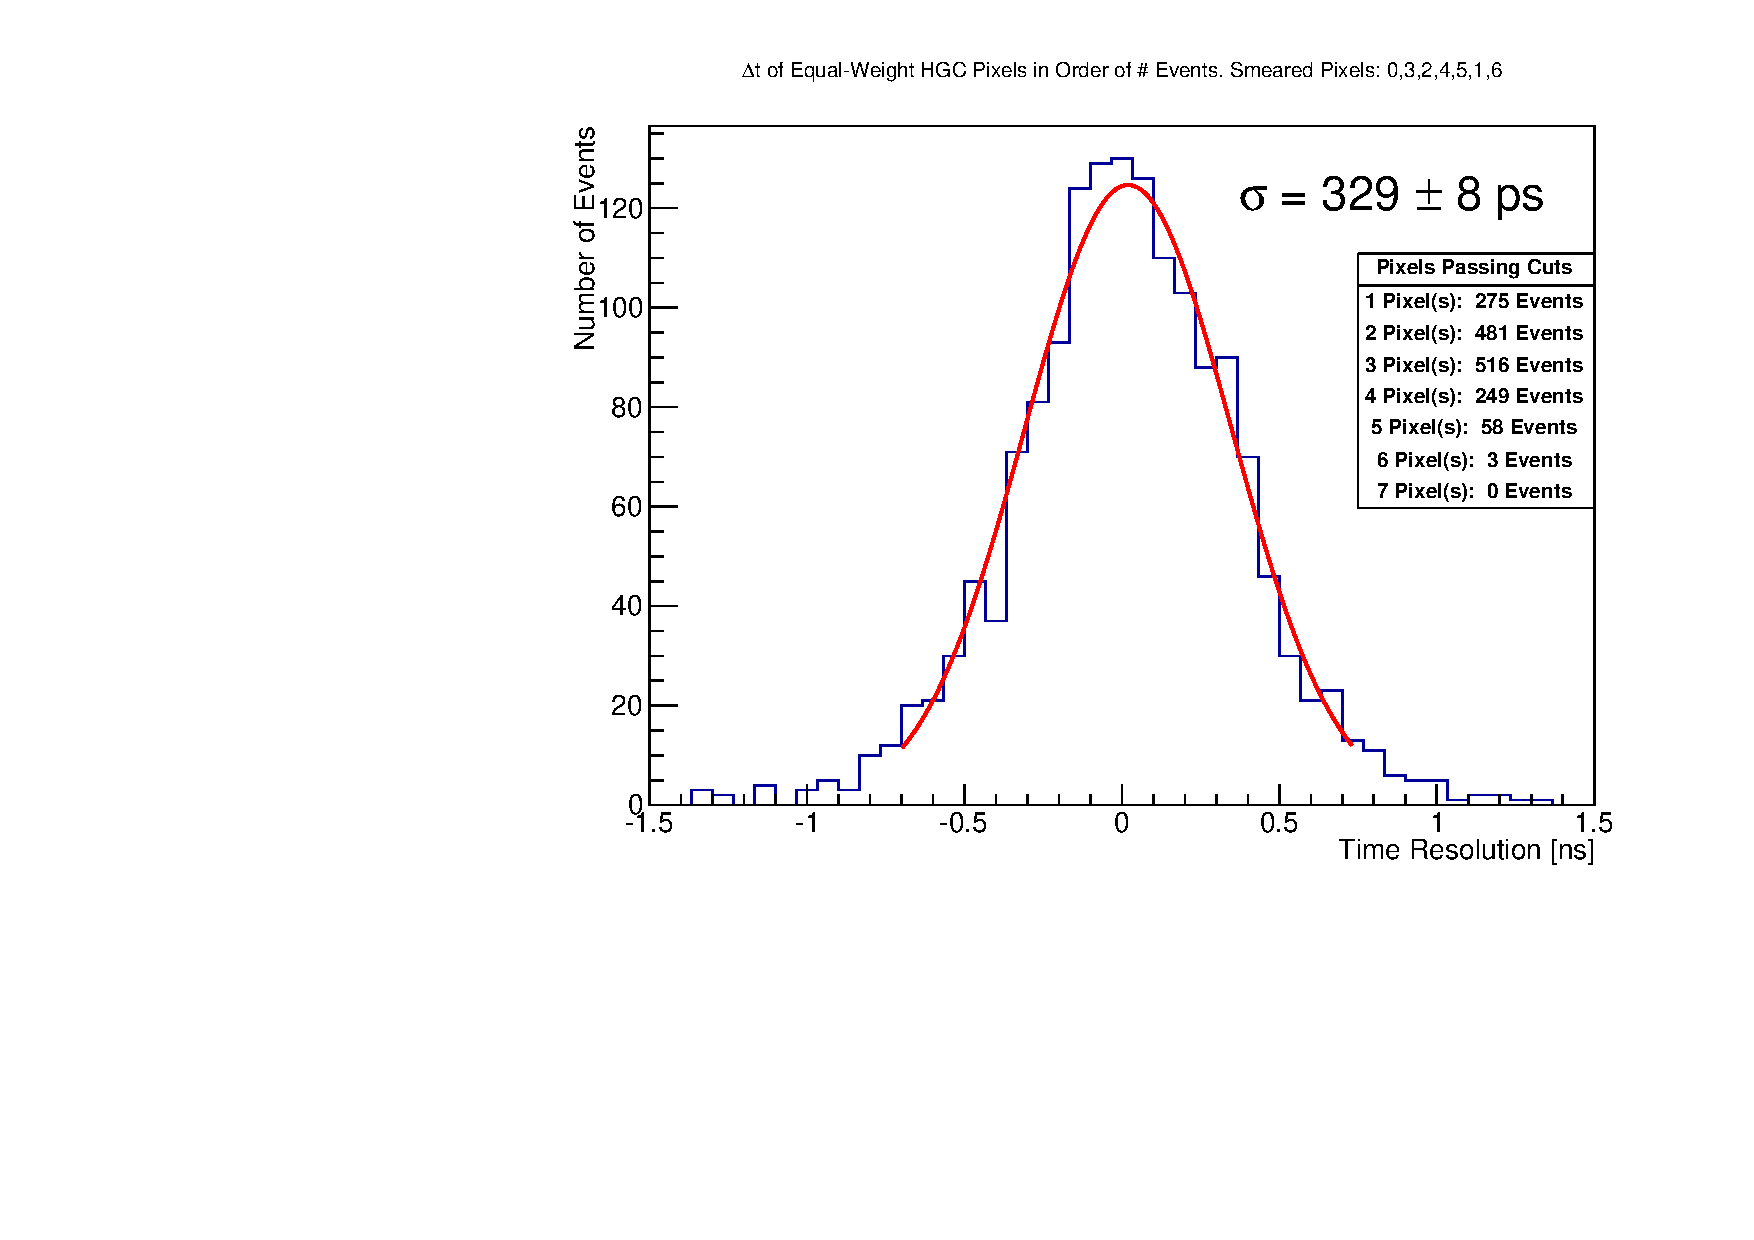
\includegraphics[width=0.4\textwidth]{SKIROC/SKIROC_7_Pixels.pdf}
	\caption{Adding in pixels in decreasing events order.
		Each has been smeared by 500 ps.}
	\label{fig:500psAll}
\end{figure}

In order to simulate another HGC layer, the Photonis MCP was smeared to 330 ps and combined with the $\Delta t$ values that were used to populate the final histogram in Figure \ref{fig:500psAll}. The Photonis TOF and combined TOF histograms are given in Figures \ref{fig:500psMCP} and \ref{fig:500psHGCMCP}.

\begin{figure}[h]
\centering
\begin{minipage}[t]{0.49\textwidth}
	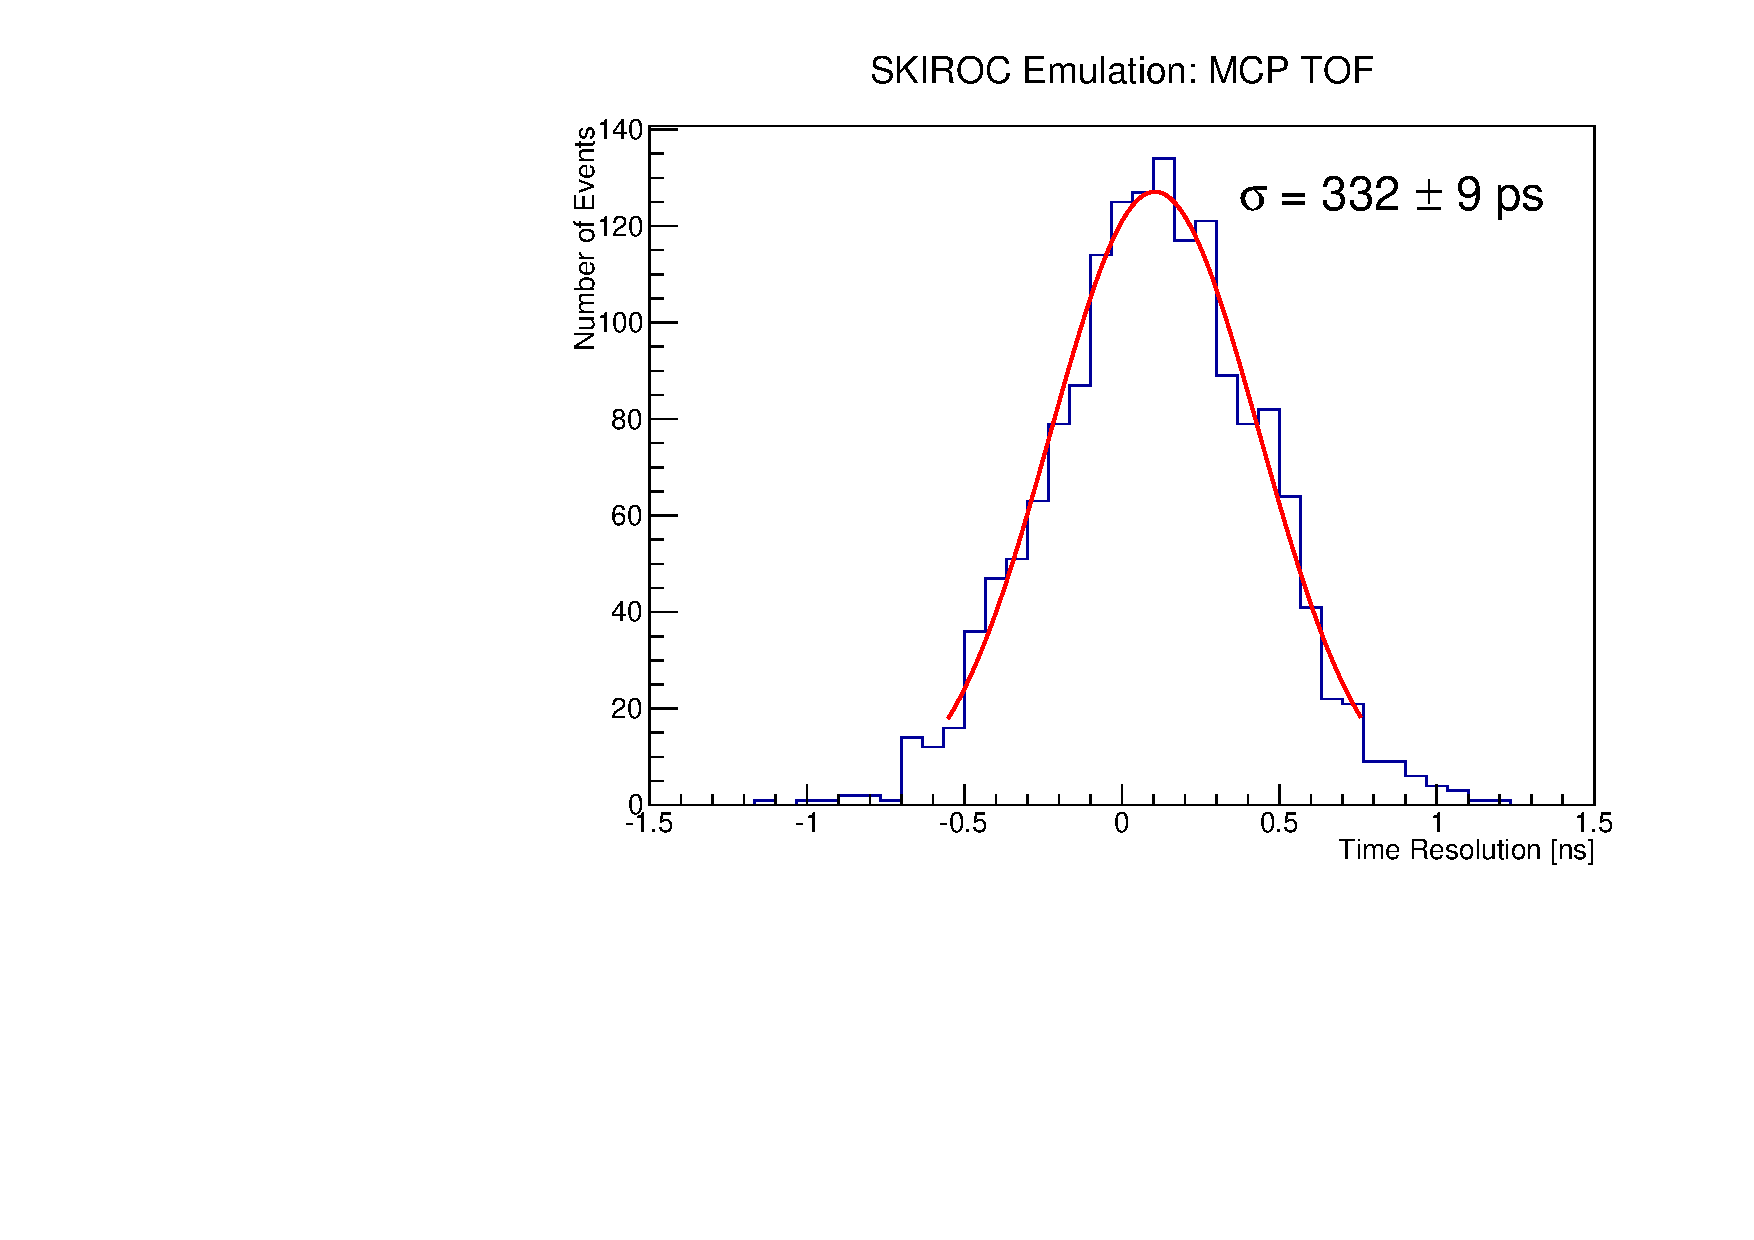
\includegraphics[width=\linewidth]{SKIROC/deltaTMCPSmear.pdf}
	\caption{TOF histogram for Photonis MCP smeared to 330 ps.}
	\label{fig:500psMCP}
\end{minipage} \hfill
\begin{minipage}[t]{0.49\textwidth}
	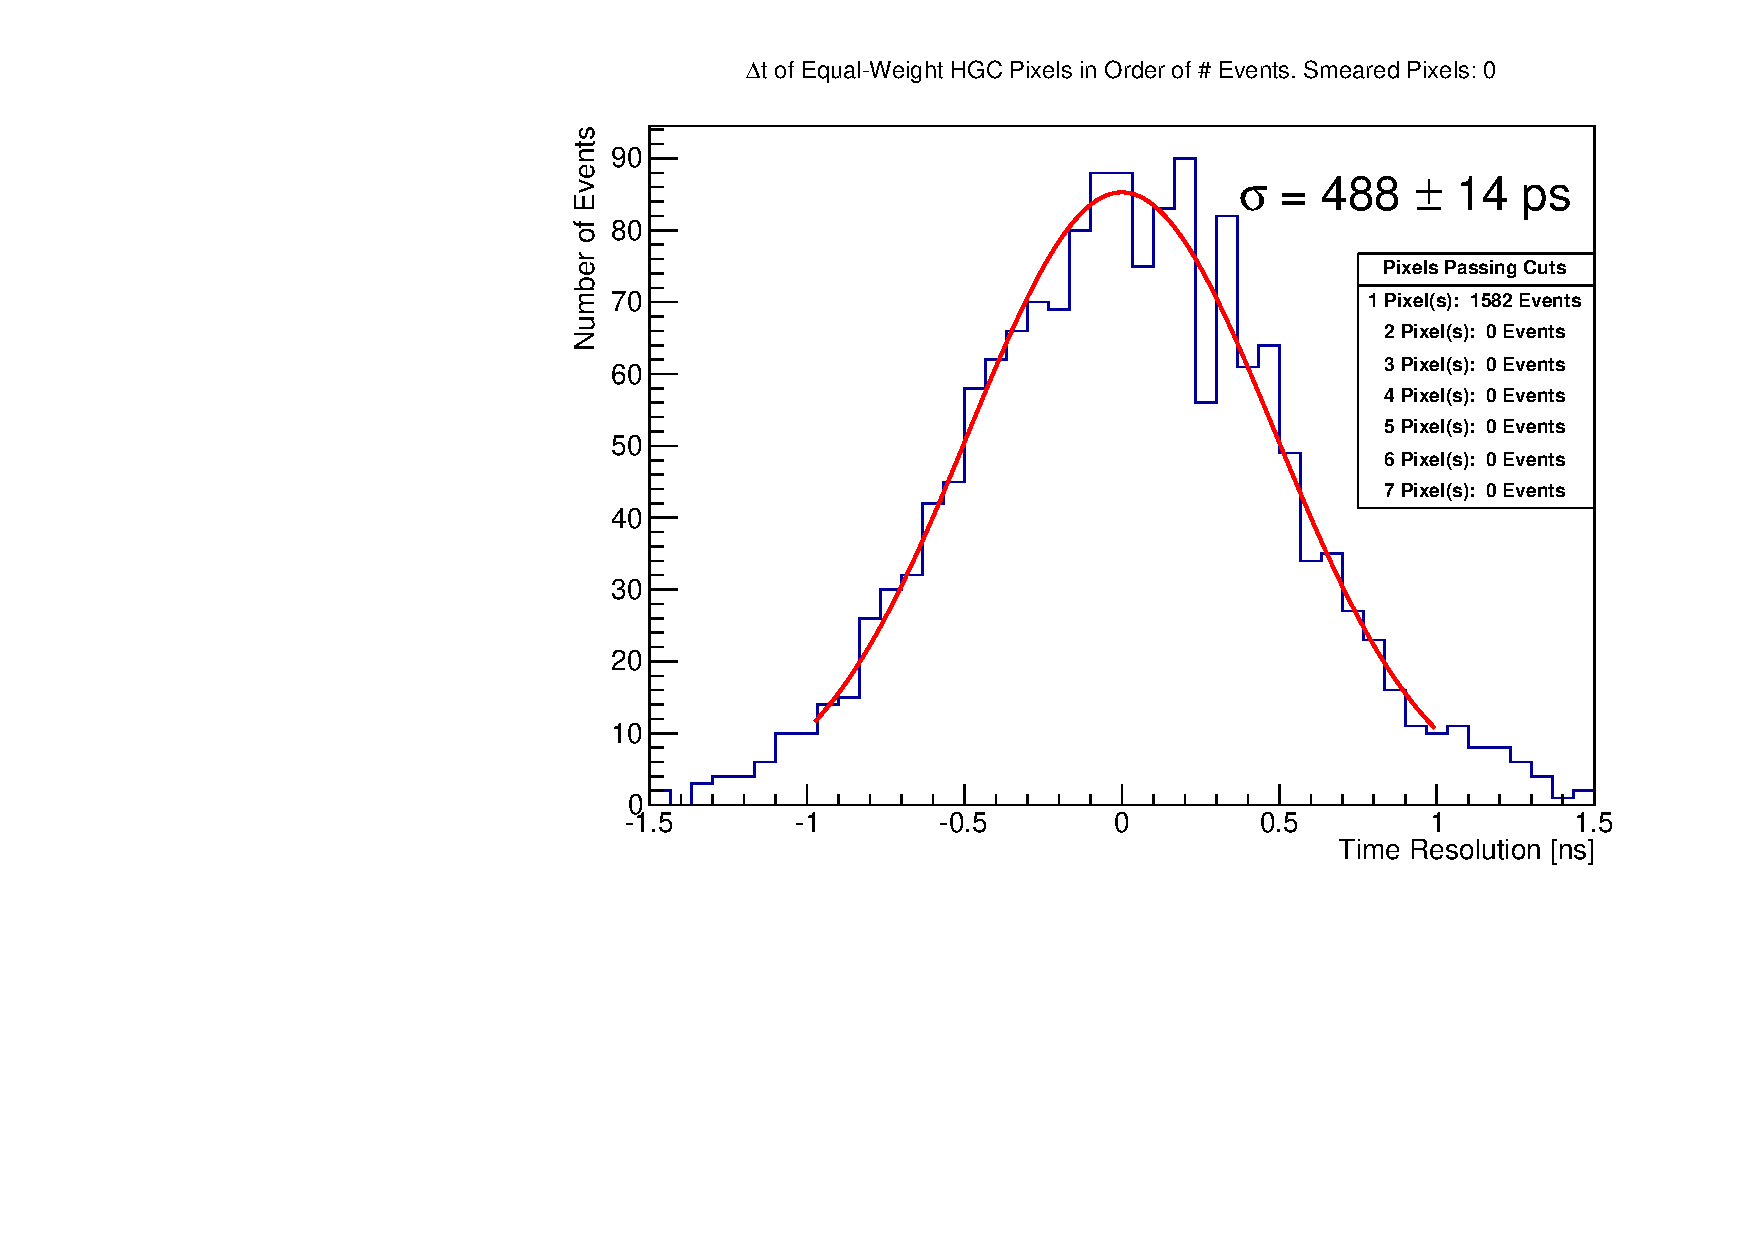
\includegraphics[width=\linewidth]{SKIROC/SKIROC_1_Pixels.pdf}
	\caption{TOF histogram, equally weighting smeared HGC layer and Photonis.}
	\label{fig:500psHGCMCP}
\end{minipage}
\end{figure}

\subsubsection{Add Pixels Individually: Exclude Center Pixel}


\subsection{Minimize $\chi^2$ or Maximize Log-Likelihood}
------------------------Move this subsection somewhere more appropriate-----------------------

possibly make it subsection 3.4

\section{Time of Flight Between HGC and Photonis}

\section{Preliminary Results and Further Research}
I am currently using my analysis code for the HGC and Photonis MCP to look at how these time resolutions change for different configurations (i.e. absorber type, spacing, and thickness; beam energy; etc). 

The next steps in the data analysis include...



%%% The following is a multi-figure example %%%
\begin{comment}
\begin{figure}[h]
\centering
	\begin{minipage}[t]{.5\textwidth} % [t] aligns at top of minipage instead of centering it
	\centering
	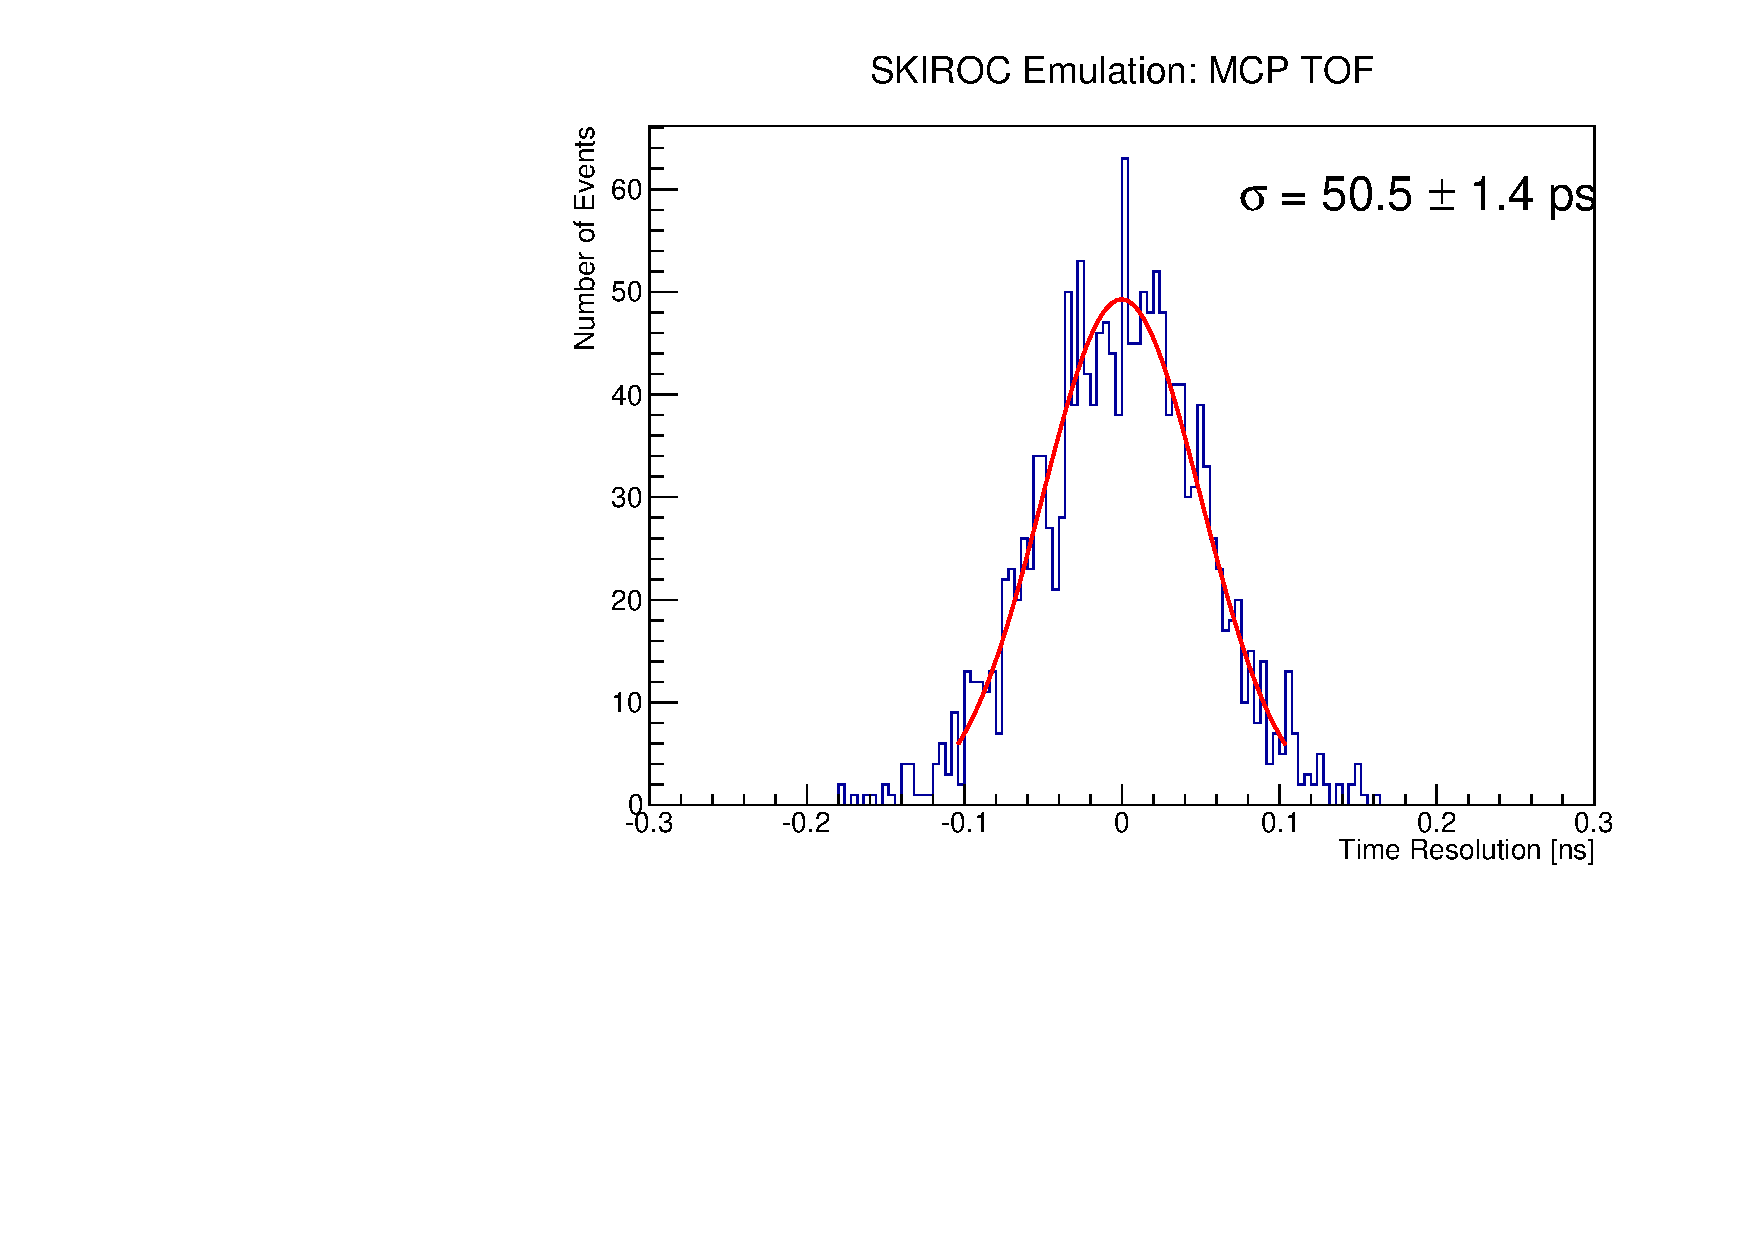
\includegraphics[width=\linewidth]{deltaTMCPSmear.pdf}
	\caption{Caption goes here}
	\label{peaks1}
	\end{minipage}\hfill
	\begin{minipage}[t]{.5\textwidth}
	\centering
	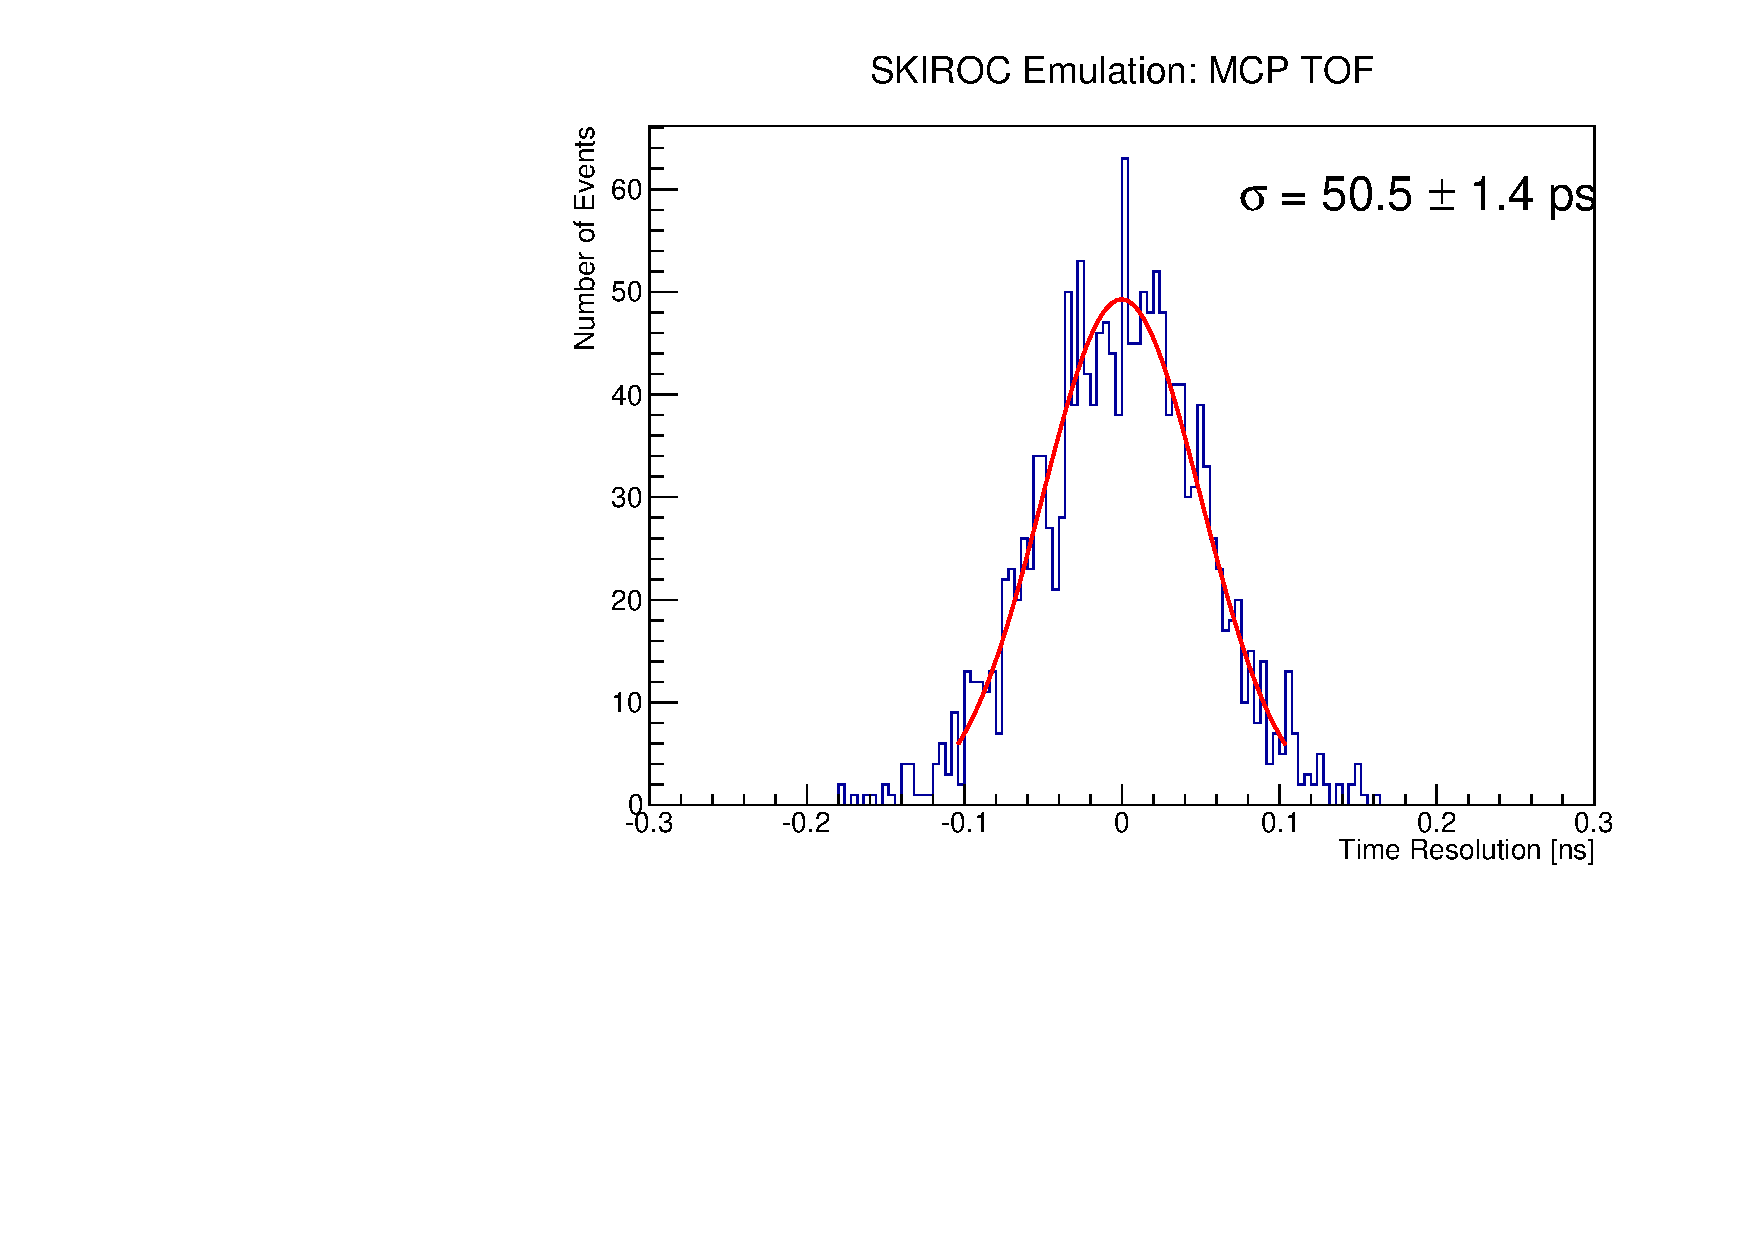
\includegraphics[width=\linewidth]{deltaTMCPSmear.pdf}
	\caption{Caption goes here}
	\label{peaks2}
	\end{minipage}
\end{figure}

look at \ref{peaks1} and \ref{peaks2}.
\end{comment}


\newpage
\printbibliography

\end{document}
